\documentclass[a4paper,twoside,12pt]{book}

\usepackage[usenames,dvipsnames]{xcolor}


%% === nezbytné balíčky:
\usepackage{lmodern}
% \usepackage[T1]{fontenc}    % kódování písma
%\usepackage[IL2]{fontenc}  % kódování písma

\usepackage[utf8]{inputenc}     % vstupní znaková sada tohoto dokumentu: UTF-8
%\usepackage[cp1250]{inputenc}  % vstupní znaková sada tohoto dokumentu: Windows 1250
%\usepackage[latin2]{inputenc}  % vstupní znaková sada tohoto dokumentu: ISO Latin 2

\usepackage[czech]{babel} % česky psaná práce, typografická pravidla. Překládejte pomocí "latex.exe" nebo "pdflatex.exe"
%\usepackage{czech} % česky psaná práce. Překládejte pomocí "pdfCSlatex.exe" ("cslatex.exe" asi bude mít problém s balíkem geometry)

\usepackage[a4paper, hmarginratio=3:2]{geometry} % využití A4 stránky a nastavení okrajů (u vazby bude širší)

\usepackage{pdfpages} % pokud nemáte formulář "Zadání bak./dipl. práce" naskenovaný jako PDF, tak ZAKOMENTUJTE
\usepackage[hidelinks]{hyperref} % v PDF budou klikací odkazy ("hidelinks" je nebude rámovat)

%% === balíčky, které se mohou hodit:
%\usepackage{encxvlna} % postará se o spojky a předložky, které dle českých pravidel nesmí být na konci řádku. Dokumentace: http://texdoc.net/texmf-dist/doc/generic/encxvlna/encxvlna.pdf (chová se správně k "vnitřku" listings?)

\usepackage{graphicx} % balíček pro vkládání rastrových grafických souborů (PNG apod.)
%\usepackage{epsfig} % balíčky pro vkládání grafických souborů typu EPS
% \usepackage{float} % rozšířené možnosti umístění obrázků
% \restylefloat{table}
\usepackage{pifont}

%\usepackage{caption} % pro popisky obrázků, tabulek atd.

\usepackage{tabularx} % rozšířené možnosti tabulek
\usepackage{longtable}
\renewcommand{\arraystretch}{1.3}

% \usepackage{tabu} % jiný balík pro rozšířené možnosti tabulek

\usepackage{listings}  % balíček vhodný pro ukázky zdrojového kódu v~textu práce/příloh. Nutno nastavit! http://ftp.cvut.cz/tex-archive/macros/latex/contrib/listings/listings.pdf
% \usepackage[autoload=true]{jlcode}

\usepackage{amsmath,amsfonts,amssymb}

% \usepackage{color} % pro možnost barevného textu
%\usepackage{fancybox} % umožňuje pokročilé rámečkování
\usepackage{url}
\usepackage{bm}
\usepackage{hyperref}
\usepackage{threeparttable}
%\usepackage{index} % nutno použít v případě tvorby rejstříku balíčkem makeindex
%\newindex{default}{idx}{ind}{Rejstřík} % zavádí rejstřík v případě použití balíku index
\usepackage{csquotes}
\MakeOuterQuote{"}

\frenchspacing % za větou bude mezislovní mezera (v anglických textech je mezera za větou delší)
\widowpenalty=1000 % "síla" zákazu vdov (= jeden řádek ze začátku odstavce na konci stránky)
\clubpenalty=1000 % "síla" zákazu sirotků (= jeden řádek/slovo z konce odstavce samostatně na začátku stránky)
\brokenpenalty=1000 % "síla" zákazu zlomu stránky za řádkem, který má na konci rozdělené slovo

\topmargin=-15mm      % horní okraj trochu menší
\textwidth=150mm      % šířka textu na stránce
\textheight=240mm     % "výška" textu na stránce


\pagenumbering{arabic} % číslování stránek arabskými číslicemi
\pagestyle{plain}      % stránky číslované dole uprostřed

\parindent=0pt % odsazení 1. řádku odstavce
\parskip=7pt   % mezera mezi odstavci

%% --- zde jsou zavedeny některé "konstanty" - některé musíte změnit! --- %%
\newcommand{\cvut}{České vysoké učení technické v~Praze}
\newcommand{\fjfi}{Fakulta jaderná a fyzikálně inženýrská}
\newcommand{\ksi}{Katedra softwarového inženýrství}
\newcommand{\km}{Katedra matematiky}
\newcommand{\program}{Aplikace přírodních věd} % změňte, pokud máte jiný stud. program
\newcommand{\obor}{Aplikace informatiky v přírodních vědách} % změňte, pokud máte kurzívujiný obor

\newcommand{\druh}{Diplomová práce} % nebo "Diplomová práce"
\newcommand{\woman}{a} % pokud jste ŽENA, ZMĚŇTE na: ...{\woman}{a} (je to do Prohlášení)

\newcommand{\logoCVUT}{
\includegraphics{symbol_cvut_konturova_verze_cb.pdf}} % logo ČVUT -- podle grafického manuálu ČVUT platného od prosince 2016. Pokud nevyhovuje PDF-verze, tak použijte jinou variantu loga: https://www.cvut.cz/logo-a-graficky-manual -> "Symbol a logo ČVUT v Praze"). Pokud chcete logo úplně vynechat, zadejte místo "\includegraphics{...}" text "\vspace{35mm}"

% přesně podle formuláře "Zadání bak./dipl. práce" VYPLŇTE:
\newcommand{\nazevczT}{Analýza příčin vzniku shrinku produktů společnosti na základě logistických dat}    % český název práce (přesně podle zadání!)
\newcommand{\nazevenT}{Root Cause Analysis of Shrinkage Based on Logistics Data}          % anglický název práce (přesně podle zadání!)
\newcommand{\nazevcz}{Analýza příčin vzniku shrinku produktů společnosti na základě logistických dat}    % český název práce (přesně podle zadání!)
\newcommand{\nazeven}{Root Cause Analysis of Shrinkage Based on Logistics Data}          % anglický název práce (přesně podle zadání!)
\newcommand{\autor}{Bc. Anna Radová}   % vyplňte své jméno a příjmení (s akademickým titulem, máte-li jej)
\newcommand{\vedouci}{Ing. Martin Plajner, Ph.D.} % vyplňte jméno a příjmení vedoucího práce, včetně titulů, např.: Doc. Ing. Ivo Malý, Ph.D.
\newcommand{\pracovisteVed}{Oddělení matematické teorie rozhodování, Ústav teorie informace a automatizace AV ČR, v.v.i.} % ZMĚŇTE, pokud vedoucí Vaší práce není z KSI
\newcommand{\konzultant}{--} % POKUD MÁTE určeného konzultanta, NAPIŠTE jeho jméno a příjmení
\newcommand{\pracovisteKonz}{--} % POKUD MÁTE konzultanta, NAPIŠTE jeho pracoviště

% podle skutečnosti VYPLŇTE:
\newcommand{\rok}{2023}  % rok odevzdání práce (jen rok odevzdání, nikoli celý akademický rok!)
\newcommand{\kde}{Praze} % studenti z Děčína ZMĚNÍ na: "Děčíně" (doplní se k "prohlášení")

\newcommand{\klicova}{Datová analýza, Logistika}   % zde NAPIŠTE česky max. 5 klíčových slov
\newcommand{\keyword}{Data Analysis, Logistics}       % zde NAPIŠTE anglicky max. 5 klíčových slov (přeložte z češtiny)
\newcommand{\abstrCZ}{}

% zde NAPIŠTE abstrakt v češtině (cca 7 vět, min. 80 slov)
\newcommand{\abstrEN}{} % zde NAPIŠTE abstrakt v angličtině

\newcommand{\prohlaseni}{Prohlašuji, že jsem svou bakalářskou práci vypracoval\woman{} samostatně a použil\woman{} jsem pouze podklady (literaturu, projekty, SW atd.) uvedené v přiloženém seznamu.} % text prohlášení můžete mírně upravit :-)

\newcommand{\podekovani}{Chtěla bych poděkovat doktoru Ing. Martinu Plajnerovi, Ph.D. za vedení mé diplomové práce, za cenné rady, připomínky a trpělivost během tvorby této práce a za čas strávený touto pomocí. Dále děkuji své rodině a manželovi za obrovkou podporu při psaní práce a během celého studia.} % NAPIŠTE poděkování, např. svému vedoucímu:
% Děkuji Ing. Eleonoře Krtečkové, Ph.D. za vedení mé bakalářské práce a za podnětné návrhy, které ji obohatily.
% NEBO:
% Děkuji vedoucímu práce doc. Pafnutijovi Snědldítětikaši, Ph.D. za neocenitelné rady a pomoc při tvorbě bakalářské práce.

\newcommand{\ti}{\textit} % zkrácený příkaz pro kurzívu
\newcommand{\tb}{\textbf} % zkrácený příkaz pro tučné písmo
\newcommand{\tn}{\texttt} % zkrácený příkaz pro neproporcionalni písmo


% Vzhled kódu
\renewcommand{\lstlistingname}{Kód}
%New colors defined below
\definecolor{julia}{rgb}{0.12,0.6,0.08}
\definecolor{julia}{rgb}{0.12,0.6,0.08}
\definecolor{chromeyellow}{rgb}{1.0, 0.65, 0.0}
\definecolor{byzantine}{rgb}{0.74, 0.2, 0.64}
\definecolor{airforceblue}{rgb}{0.36, 0.54, 0.66}
\definecolor{backcolor}{rgb}{0.95,0.95,0.95}
\definecolor{border}{rgb}{0.98,0.98,0.98}

% Takhle se pouziva pro ukazky kodu
% \begin{lstlisting}[caption=Definice metody size pro dataset Iris, label=Kod:ImSiz]
%     size(::Iris) = (150, 0, 0)
% \end{lstlisting}

% napise julia> barevne
\newcommand{\jul}{\textcolor{julia}{julia> }}


\newenvironment{repl}
{\fontfamily{cmvtt}\selectfont \begin{mdframed}

}{\end{mdframed}}

\usepackage[linewidth=1pt]{mdframed}


\newcolumntype{L}{>{\centering\arraybackslash}m{2cm}}
\newcolumntype{N}{>{\centering\arraybackslash}m{1.7cm}}
\newcolumntype{M}{>{\centering\arraybackslash}m{1.6cm}}
\newcolumntype{K}{>{\centering\arraybackslash}m{1.5cm}}
\newcolumntype{S}{>{\centering\arraybackslash}m{1cm}}
\renewcommand{\arraystretch}{1.3}

\newcommand{\cmark}{\textcolor{green!80!black}{\ding{51}}}
\newcommand{\xmark}{\textcolor{red}{\ding{55}}}




% Listing style
\lstdefinelanguage{julia}
{%
%
% julia's keywords:
%
morekeywords=[1]
{%
abstract type,baremodule,begin,break,catch,ccall,const,continue,do,else,elseif,%
end,export,finally,for,function,global,if,import,in,isa,let,local,macro,module,%
mutable struct,primitive type,quote,return,struct,try,using,where,while, function%
},%
%
% julia's literals:
%
morekeywords=[2]
{%
ARCH,ARGS,Apr,April,Aug,August,BINDIR,CPU_NAME,CPU_THREADS,C_NULL,DEPOT_PATH,%
DL_LOAD_PATH,Dec,December,ENDIAN_BOM,ENV,Feb,February,Fri,Friday,I,%
ISODateFormat,ISODateTimeFormat,ISOTimeFormat,Inf,Inf16,Inf32,Inf64,%
InsertionSort,JIT,Jan,January,Jul,July,Jun,June,KERNEL,LOAD_PATH,MACHINE,Mar,%
March,May,MergeSort,Mon,Monday,NaN,NaN16,NaN32,NaN64,Nov,November,Oct,October,%
PROGRAM_FILE,QuickSort,RFC1123Format,RTLD_DEEPBIND,RTLD_FIRST,RTLD_GLOBAL,%
RTLD_LAZY,RTLD_LOCAL,RTLD_NODELETE,RTLD_NOLOAD,RTLD_NOW,RoundDown,%
RoundFromZero,RoundNearest,RoundNearestTiesAway,RoundNearestTiesUp,RoundToZero,%
RoundUp,STDLIB,Sat,Saturday,Sep,September,Sun,Sunday,Thu,Thursday,Tue,Tuesday,%
VERSION,WORD_SIZE,Wed,Wednesday,catalan,devnull,dlext,e,eulergamma,false,%
golden,im,missing,nothing,pi,stderr,stdin,stdout,true,undef,γ,π,φ,ℯ%
},%
%
% julia's built-ins:
%
morekeywords=[3]
{%
AbstractArray,AbstractChannel,AbstractChar,AbstractDict,AbstractDisplay,%
AbstractFloat,AbstractIrrational,AbstractLogger,AbstractMatrix,AbstractREPL,%
AbstractRNG,AbstractRange,AbstractSerializer,AbstractSet,AbstractSparseArray,%
AbstractSparseMatrix,AbstractSparseVector,AbstractString,AbstractUnitRange,%
AbstractVecOrMat,AbstractVector,AbstractWorkerPool,Adjoint,Any,ArgumentError,%
Array,AssertionError,Atomic,Base64DecodePipe,Base64EncodePipe,BasicREPL,%
Bidiagonal,BigFloat,BigInt,BitArray,BitMatrix,BitSet,BitVector,Bool,%
BoundsError,BroadcastStyle,BunchKaufman,CachingPool,CapturedException,%
CartesianIndex,CartesianIndices,Cchar,Cdouble,Cfloat,Channel,Char,Cholesky,%
CholeskyPivoted,Cint,Cintmax_t,Clong,Clonglong,ClusterManager,Cmd,CodeInfo,%
CodeInstance,Colon,Complex,ComplexF16,ComplexF32,ComplexF64,CompositeException,%
Condition,ConsoleLogger,Cptrdiff_t,Cshort,Csize_t,Cssize_t,Cstring,Cuchar,%
Cuint,Cuintmax_t,Culong,Culonglong,Cushort,Cvoid,Cwchar_t,Cwstring,DataType,%
Date,DateFormat,DatePeriod,DateTime,Day,DenseArray,DenseMatrix,DenseVecOrMat,%
DenseVector,Diagonal,Dict,DimensionMismatch,Dims,DivideError,DomainError,%
EOFError,Eigen,Enum,ErrorException,Event,Exception,ExponentialBackOff,Expr,%
FDWatcher,FILE,Factorization,FileMonitor,Float16,Float32,Float64,FolderMonitor,%
Function,Future,GeneralizedEigen,GeneralizedSVD,GeneralizedSchur,GenericArray,%
GenericDict,GenericOrder,GenericSet,GenericString,GitConfig,GitRepo,GlobalRef,%
GotoNode,HMAC_CTX,HTML,Hermitian,Hessenberg,Hour,IO,IOBuffer,IOContext,%
IOStream,IPAddr,IPv4,IPv6,IdDict,IndexCartesian,IndexLinear,IndexStyle,%
InexactError,InitError,Int,Int128,Int16,Int32,Int64,Int8,Integer,%
InterruptException,InvalidStateException,Irrational,KeyError,LAPACKException,%
LDLt,LQ,LU,LinRange,LineEditREPL,LineInfoNode,LineNumberNode,LinearIndices,%
LoadError,LogLevel,LowerTriangular,MIME,Matrix,MersenneTwister,Method,%
MethodError,MethodInstance,Microsecond,Millisecond,Minute,Missing,%
MissingException,Module,Month,NTuple,NamedTuple,Nanosecond,NewvarNode,Nothing,%
NullLogger,Number,OrdinalRange,OutOfMemoryError,OverflowError,Pair,%
PartialQuickSort,Period,PermutedDimsArray,PhiCNode,PhiNode,PiNode,Pipe,%
PollingFileWatcher,PosDefException,ProcessExitedException,%
ProcessFailedException,Ptr,QR,QRPivoted,QuoteNode,RandomDevice,%
RankDeficientException,Rational,RawFD,ReadOnlyMemoryError,Real,ReentrantLock,%
Ref,Regex,RegexMatch,RemoteChannel,RemoteException,RoundingMode,SHA1_CTX,%
SHA224_CTX,SHA256_CTX,SHA2_224_CTX,SHA2_256_CTX,SHA2_384_CTX,SHA2_512_CTX,%
SHA384_CTX,SHA3_224_CTX,SHA3_256_CTX,SHA3_384_CTX,SHA3_512_CTX,SHA512_CTX,%
SSAValue,SVD,Schur,Second,SegmentationFault,Serializer,Set,SharedArray,%
SharedMatrix,SharedVector,Signed,SimpleLogger,SingularException,Slot,%
SlotNumber,Some,SparseMatrixCSC,SparseVector,SpinLock,StackFrame,%
StackOverflowError,StackTrace,StepRange,StepRangeLen,StreamREPL,StridedArray,%
StridedMatrix,StridedVecOrMat,StridedVector,String,StringIndexError,SubArray,%
SubString,SubstitutionString,SymTridiagonal,Symbol,Symmetric,SystemError,%
TCPSocket,Task,TaskFailedException,TestSetException,Text,TextDisplay,Time,%
TimePeriod,TimeType,TimeZone,Timer,TmStruct,Transpose,Tridiagonal,Tuple,%
TypeError,TypeVar,TypedSlot,UDPSocket,UInt,UInt128,UInt16,UInt32,UInt64,UInt8,%
UTC,UUID,UndefInitializer,UndefKeywordError,UndefRefError,UndefVarError,%
UniformScaling,Union,UnionAll,UnitLowerTriangular,UnitRange,%
UnitUpperTriangular,Unsigned,UpperHessenberg,UpperTriangular,UpsilonNode,Val,%
Vararg,VecElement,VecOrMat,Vector,VersionNumber,WeakKeyDict,WeakRef,Week,%
WorkerConfig,WorkerPool,Year,ZeroPivotException,%
DatasetName,Tabular,Split, GrayImage, MLImage,Image, Classification, Regression,%
Iris, Adult, MNIST, Nuclear, Gisette, Labels, Ionosphere, Train, L2, Boston 
},%
%
% julia's macros:
%
morekeywords=[4]
{%
@MIME_str,@NamedTuple,@__DIR__,@__FILE__,@__LINE__,@__MODULE__,@__dot__,%
@allocated,@assert,@async,@b_str,@big_str,@boundscheck,@ccall,@cfunction,@cmd,%
@code_llvm,@code_lowered,@code_native,@code_typed,@code_warntype,%
@dateformat_str,@debug,@deprecate,@distributed,@doc,@doc_str,@dump,@edit,%
@elapsed,@enum,@error,@eval,@evalpoly,@everywhere,@fastmath,@fetch,@fetchfrom,%
@functionloc,@generated,@gensym,@goto,@html_str,@inbounds,@inferred,@info,%
@inline,@int128_str,@ip_str,@isdefined,@label,@less,@logmsg,@macroexpand,%
@macroexpand1,@md_str,@noinline,@nospecialize,@polly,@printf,@profile,@r_str,%
@raw_str,@s_str,@show,@simd,@spawn,@spawnat,@specialize,@sprintf,@static,@sync,%
@task,@test,@test_broken,@test_deprecated,@test_logs,@test_nowarn,@test_skip,%
@test_throws,@test_warn,@testset,@text_str,@threadcall,@threads,@time,@timed,%
@timev,@uint128_str,@v_str,@var,@view,@views,@warn,@which%
},%
%
% julia's functions:
%
morekeywords=[5]
{%
BLAS,Base,Base64,Broadcast,CRC32c,Compiler,Core,Dates,DelimitedFiles,%
Distributed,Docs,FileWatching,FormatMessage,GC,GetLastError,IR,%
InteractiveUtils,Intrinsics,Iterators,LAPACK,LibGit2,Libc,Libdl,LinearAlgebra,%
Logging,Main,Markdown,MathConstants,Meta,Mmap,PipeBuffer,Printf,Profile,REPL,%
Random,SHA,Serialization,SharedArrays,Sockets,SparseArrays,StackTraces,%
SuiteSparse,Sys,Test,Threads,UUIDs,Unicode,__precompile__,abs,abs2,abs_float,%
abspath,accept,accumulate,accumulate!,acos,acosd,acosh,acot,acotd,acoth,acsc,%
acscd,acsch,add_float,add_float_fast,add_int,add_ptr,addprocs,adjoint,adjoint!,%
adjust,all,all!,allunique,and_int,angle,any,any!,append!,applicable,apropos,%
argmax,argmin,arraylen,ascii,asec,asecd,asech,ashr_int,asin,asind,asinh,%
asyncmap,asyncmap!,atan,atand,atanh,atexit,atomic_add!,atomic_and!,atomic_cas!,%
atomic_fence,atomic_max!,atomic_min!,atomic_nand!,atomic_or!,atomic_sub!,%
atomic_xchg!,atomic_xor!,atreplinit,axes,axpby!,axpy!,backtrace,base64decode,%
base64encode,basename,big,bind,binomial,bitcast,bitrand,bitreverse,bitrotate,%
bitstring,blockdiag,broadcast,broadcast!,broadcast_axes,%
broadcast_preserving_zero_d,broadcastable,bswap,bswap_int,bunchkaufman,%
bunchkaufman!,bytes2hex,bytesavailable,calloc,canonicalize,cat,catch_backtrace,%
cbrt,cd,ceil,ceil_llvm,cglobal,channel_from_id,check_same_host,checkbounds,%
checked_sadd_int,checked_sdiv_int,checked_smul_int,checked_srem_int,%
checked_ssub_int,checked_uadd_int,checked_udiv_int,checked_umul_int,%
checked_urem_int,checked_usub_int,checkindex,chmod,cholesky,cholesky!,chomp,%
chop,chown,circcopy!,circshift,circshift!,cis,clamp,clamp!,cld,clear!,%
clipboard,close,cluster_cookie,cmp,coalesce,code_llvm,code_lowered,code_native,%
code_typed,code_warntype,codepoint,codeunit,codeunits,collect,complex,cond,%
condskeel,conj,conj!,connect,contains,convert,copy,copy!,copy_transpose!,%
copysign,copysign_float,copyto!,cos,cosc,cosd,cosh,cospi,cot,cotd,coth,count,%
count!,count_ones,count_zeros,countfrom,countlines,cp,cpu_info,cpu_summary,%
crc32c,cross,csc,cscd,csch,ctime,ctlz_int,ctpop_int,cttz_int,cumprod,cumprod!,%
cumsum,cumsum!,current_logger,current_task,cycle,datetime2julian,datetime2rata,%
datetime2unix,day,dayabbr,dayname,dayofmonth,dayofquarter,dayofweek,%
dayofweekofmonth,dayofyear,daysinmonth,daysinyear,daysofweekinmonth,deepcopy,%
default_worker_pool,deg2rad,delete!,deleteat!,denominator,deserialize,det,%
detach,detect_ambiguities,detect_unbound_args,diag,diagind,diagm,diff,digest!,%
digits,digits!,dirname,disable_logging,disable_sigint,display,displayable,%
displaysize,div,div_float,div_float_fast,divrem,dlclose,dllist,dlopen,dlopen_e,%
dlpath,dlsym,dlsym_e,doc,dot,dotview,download,drop,dropdims,droptol!,dropwhile,%
dropzeros,dropzeros!,dump,eachcol,eachindex,eachline,eachmatch,eachrow,%
eachslice,edit,eigen,eigen!,eigmax,eigmin,eigvals,eigvals!,eigvecs,eltype,%
empty,empty!,endswith,enumerate,eof,eps,eq_float,eq_float_fast,eq_int,errno,%
error,esc,escape_string,eval,evalfile,evalpoly,exit,exp,exp10,exp2,expanduser,%
expm1,exponent,extrema,factorial,factorize,falses,fd,fdio,fetch,fieldcount,%
fieldname,fieldnames,fieldoffset,fieldtype,fieldtypes,filemode,filesize,fill,%
fill!,filter,filter!,finalize,finalizer,find_library,findall,findfirst,%
findlast,findmax,findmax!,findmin,findmin!,findnext,findnz,findprev,first,%
firstdayofmonth,firstdayofquarter,firstdayofweek,firstdayofyear,firstindex,%
flatten,fld,fld1,fldmod,fldmod1,flipsign,flipsign_int,float,floatmax,floatmin,%
floor,floor_llvm,flush,flush_cstdio,fma,fma_float,foldl,foldr,foreach,fpext,%
fpiseq,fpislt,fptosi,fptoui,fptrunc,free,free_memory,frexp,fullname,%
functionloc,gcd,gcdx,gensym,get,get!,get_zero_subnormals,getaddrinfo,%
getalladdrinfo,getfield,gethostname,getindex,getipaddr,getipaddrs,getkey,%
getnameinfo,getpeername,getpid,getproperty,getsockname,givens,global_logger,%
gperm,graphemes,hasfield,hash,haskey,hasmethod,hasproperty,hcat,hessenberg,%
hessenberg!,hex2bytes,hex2bytes!,hmac_sha1,hmac_sha224,hmac_sha256,%
hmac_sha2_224,hmac_sha2_256,hmac_sha2_384,hmac_sha2_512,hmac_sha384,%
hmac_sha3_224,hmac_sha3_256,hmac_sha3_384,hmac_sha3_512,hmac_sha512,homedir,%
hour,html,htol,hton,hvcat,hypot,identity,ifelse,ignorestatus,imag,in,%
include_dependency,include_string,indexin,indexpids,init_worker,insert!,%
instances,interrupt,intersect,intersect!,inv,invmod,invoke,invperm,invpermute!,%
isa,isabspath,isabstracttype,isapple,isapprox,isascii,isassigned,isbits,%
isbitstype,isblockdev,isbsd,ischardev,iscntrl,isconcretetype,isconst,isdefined,%
isdiag,isdigit,isdir,isdirpath,isdisjoint,isdispatchtuple,isdragonfly,isempty,%
isequal,iseven,isexecutable,isexpr,isfifo,isfile,isfinite,isfreebsd,%
ishermitian,isimmutable,isinf,isinteger,isinteractive,isjsvm,isleapyear,isless,%
isletter,islink,islinklocaladdr,islinux,islocked,islowercase,ismarked,%
ismissing,ismount,ismutable,isnan,isnetbsd,isnothing,isnumeric,isodd,isone,%
isopen,isopenbsd,ispath,isperm,isposdef,isposdef!,ispow2,isprimitivetype,%
isprint,ispunct,isqrt,isreadable,isreadonly,isready,isreal,issetequal,issetgid,%
issetuid,issocket,issorted,isspace,issparse,issticky,isstructtype,issubnormal,%
issubset,issuccess,issymmetric,istaskdone,istaskfailed,istaskstarted,%
istextmime,istril,istriu,isunix,isuppercase,isvalid,iswindows,iswritable,%
isxdigit,iszero,iterate,join,join_multicast_group,joinpath,julian2datetime,%
keys,keytype,kill,kron,last,lastdayofmonth,lastdayofquarter,lastdayofweek,%
lastdayofyear,lastindex,latex,launch,lcm,ldexp,ldiv!,ldlt,ldlt!,le_float,%
le_float_fast,leading_ones,leading_zeros,leave_multicast_group,length,%
less,listen,listenany,llvmcall,lmul!,loadavg,localindices,lock,log,log10,log1p,%
log2,logabsdet,logdet,lowercase,lowercasefirst,lowrankdowndate,%
lowrankdowndate!,lowrankupdate,lowrankupdate!,lpad,lq,lq!,lshr_int,lstat,%
lstrip,lt_float,lt_float_fast,ltoh,lu,lu!,lyap,macroexpand,malloc,manage,map,%
map!,mapfoldl,mapfoldr,mapreduce,mapslices,mark,match,max,maximum,maximum!,%
maxintfloat,merge,merge!,mergewith,mergewith!,methods,methodswith,microsecond,%
millisecond,min,minimum,minimum!,minmax,minute,mkdir,mkpath,mktemp,mktempdir,%
mod,mod1,mod2pi,modf,month,monthabbr,monthday,monthname,mtime,mul!,mul_float,%
mul_float_fast,mul_int,muladd,muladd_float,mv,myid,nameof,names,nanosecond,%
ncodeunits,ndigits,ndims,ne_float,ne_float_fast,ne_int,neg_float,%
neg_float_fast,neg_int,nextfloat,nextind,nextpow,nextprod,nfields,nnz,%
nonmissingtype,nonzeros,norm,normalize,normalize!,normpath,not_int,notify,now,%
nprocs,nthreads,ntoh,ntuple,nullspace,numerator,nworkers,nzrange,objectid,%
occursin,oftype,one,ones,oneunit,only,open,operm,opnorm,or_int,ordschur,%
ordschur!,pairs,parent,parentindices,parentmodule,parse,partialsort,%
partialsort!,partialsortperm,partialsortperm!,partition,pathof,peakflops,peek,%
permute,permute!,permutedims,permutedims!,pinv,pipeline,pkgdir,pmap,pointer,%
pointer_from_objref,pointerref,pointerset,poll_fd,poll_file,pop!,popat!,%
popdisplay,popfirst!,position,powermod,precision,precompile,prepend!,prevfloat,%
prevind,prevpow,print,println,printstyled,process_exited,process_messages,%
process_running,procs,prod,prod!,product,promote,promote_rule,promote_shape,%
promote_type,propertynames,push!,pushdisplay,pushfirst!,put!,pwd,qr,qr!,%
quarterofyear,quot,rad2deg,rand,rand!,randcycle,randcycle!,randexp,randexp!,%
randn,randn!,randperm,randperm!,randstring,randsubseq,randsubseq!,range,rank,%
rata2datetime,rationalize,rdiv!,read,read!,readavailable,readbytes!,readchomp,%
readdir,readdlm,readline,readlines,readlink,readuntil,real,realloc,realpath,%
recv,recvfrom,redirect_stderr,redirect_stdin,redirect_stdout,redisplay,reduce,%
reenable_sigint,reflect!,reim,reinterpret,relpath,rem,rem2pi,rem_float,%
rem_float_fast,remote,remote_do,remotecall,remotecall_fetch,remotecall_wait,%
remoteref_id,repeat,repeated,replace,replace!,repr,reset,reshape,resize!,rest,%
rethrow,retry,reverse,reverse!,reverseind,rint_llvm,rm,rmprocs,rmul!,rot180,%
rotate!,rotl90,rotr90,round,rounding,rowvals,rpad,rsplit,rstrip,run,schedule,%
schur,schur!,sdata,sdiv_int,searchsorted,searchsortedfirst,searchsortedlast,%
sec,secd,sech,second,seek,seekend,seekstart,selectdim,send,serialize,%
set_zero_subnormals,setdiff,setdiff!,setenv,setfield!,setindex!,setprecision,%
setproperty!,setrounding,sext_int,sha1,sha224,sha256,sha2_224,sha2_256,%
sha2_384,sha2_512,sha384,sha3_224,sha3_256,sha3_384,sha3_512,sha512,shl_int,%
show,show_sexpr,showable,showerror,shuffle,shuffle!,sign,signbit,signed,%
significand,similar,sin,sinc,sincos,sincosd,sind,sinh,sinpi,sitofp,size,%
sizehint!,sizeof,skip,skipchars,skipmissing,sle_int,sleep,slt_int,something,%
sort,sort!,sortperm,sortperm!,sotrtslices,sparse,sparsevec,spdiagm,splice!,%
split,splitdir,splitdrive,splitext,splitpath,sprand,sprandn,sprint,spzeros,%
sqrt,sqrt_llvm,sqrt_llvm_fast,srem_int,stacktrace,start_worker,srtartswith,%
stat,step,strerror,strftime,stride,strides,string,stringmime,strip,strptime,%
sub_float,sub_float_fast,sub_int,sub_ptr,subtypes,success,sum,sum!,summary,%
supertype,supertypesd,svd,svd!,svdvals,svdvals!,sylvester,symdiff,symdiff!,%
symlink,systemerror,systemsleep,take,take!,takewhile,tan,tand,tanh,%
task_local_storage,tempdir,tempname,textwidth,thisind,threadhid,throw,time,%
time_ns,timedwait,titlecase,to_indices,today,tofirst,tolast,tonext,toprev,%
total_memory,touch,tr,trailing_ones,trailing_zeros,transcode,transpose,%
transpose!,tril,tril!,ttriu,triu!,trues,trunc,trunc_int,trunc_llvm,truncate,%
trylock,tryparse,tuple,typeassert,typeintersect,typejoin,typemax,typemin,%
typeof,udiv_int,uitofp,ule_int,ult_int,unescape_string,uunion,union!,unique,%
unique!,unix2datetime,unlock,unmark,unsafe_copyto!,unsafe_load,%
unsafe_pointer_to_objref,unsafe_read,unsafe_store!,unsafe_string,unsafe_trunc,%
unsafe_wrap,unsafe_wsrite,unsigned,unwatch_folder,update!,uperm,uppercase,%
uppercasefirst,uptime,urem_int,uuid1,uuid4,uuid5,uuid_version,valtype,values,%
varinfo,vcat,vec,versioninfo,view,wait,walkdir,watcah_file,watch_folder,week,%
which,widemul,widen,with,with_logger,withenv,worker_id_from_socket,workers,%
write,writedlm,xor,xor_int,year,yearmonth,yearmonthday,yield,yieldto,zero,%
zeros,ziext_int,zip, load, name, prep, preprocess, url, checksum,%
target, headers, problem, message, postprocess, getdata, split_traintest,%
split_trainvalidtest, meanstd, binarize, info
},%
%
%
sensitive=true,%
%
alsoother={$},%$%
alsodigit={_},%
%
morecomment=[l]{\#},%
morecomment=[n]{\#=}{=\#},%
%
morestring=[b]{"},%
% just activate the next command if you dont use ' as the transposition
% operator! comment out line 1283 in that case, too!
%morestring=[m]{'},%
morestring=[s]{"""}{"""},%
morestring=[s]{L"}{"},%
morestring=[s]{MIME"}{"},%
morestring=[s]{b"}{"},%
morestring=[s]{big"}{"},%
morestring=[s]{dateformat"}{"},%
morestring=[s]{doc"}{"},%
morestring=[s]{html"}{"},%
morestring=[s]{int128"}{"},%
morestring=[s]{ip"}{"},%
morestring=[s]{md"}{"},%
morestring=[s]{pkg"}{"},%
morestring=[s]{r"}{"},%
morestring=[s]{raw"}{"},%
morestring=[s]{s"}{"},%
morestring=[s]{text"}{"},%
morestring=[s]{uint128"}{"},%
morestring=[s]{v"}{"},%
morestring=[s]{var"}{"},%
%
}[keywords,comments,strings]

\definecolor{jlbase}{RGB}{68, 68, 68}       % julia's base color
\definecolor{jlkeyword}{RGB}{230, 9, 72}    % julia's keywords
\definecolor{jlliteral}{RGB}{11, 195, 212}  % julia's literals
\definecolor{jlbuiltin}{RGB}{7, 94, 235}    % julia's built-ins
\definecolor{jlmacros}{RGB}{255, 166, 0}    % julia's macros
\definecolor{jlfunctions}{RGB}{11, 156, 25} % julia's functions
\definecolor{jlcomment}{RGB}{136, 136, 136} % julia's comments
\definecolor{jlstrnum}{RGB}{255, 166, 0}    % julia's strings or numbers
\definecolor{jlop}{RGB}{68, 68, 68}         % julia's operators

\lstdefinestyle{juliastyle}{
    captionpos = b,
    basicstyle=\ttfamily\footnotesize, 
    tabsize = 2,
    lineskip = -1.5pt,
    extendedchars = true,
    breaklines = true,
    upquote = true,
    tabsize = 4,
    aboveskip = {0.5\baselineskip},
    belowskip = {0.5\baselineskip},
    rulecolor=\color{Black},
    frame = shadowbox,
    rulesepcolor = \color{white!50!gray},
    columns = fixed,
    linewidth = \textwidth,
    xleftmargin = {0.05\textwidth},
    xrightmargin = {0.05\textwidth},
    keywordstyle={[1]\color{jlkeyword}\bfseries},
    keywordstyle={[2]\color{jlliteral}},
    keywordstyle={[3]\color{jlbuiltin}},
    keywordstyle={[4]\color{jlmacros}},
    keywordstyle={[5]\color{jlfunctions}},
    commentstyle={\color{jlcomment}},
    stringstyle={\color{jlstrnum}},
    identifierstyle={\color{jlbase}},
    showstringspaces=false,
}
\lstset{style = juliastyle, language = julia}


\lstdefinelanguage{juliarepl}
{%
% Purple
morekeywords=[1]{
    DatasetName, using%
},%
% Light blue
morekeywords=[2]{},%
% Blue
morekeywords=[3]{
    Image, Tabular, v1.6, pkg, add
},
% Yellow
morekeywords=[4]{
    CIFAR10, CIFAR100, SVHN2, FashionMNIST, MNIST,
},
% Green
morekeywords=[5]{
    julia,
    ColorImage, GrayImage, Abalone, Adult, Boston, Carevaluation, Forestfires,
    Gisette, Ionosphere, Iris, Nuclear, Wine,
    listdatasets, info,
},
}[keywords]

\lstdefinelanguage{juliarepl2}
{%
% Purple
morekeywords=[1]{
    using
},%
% Light blue
morekeywords=[2]{Info},%
% Blue
morekeywords=[3]{
    Vector, Bool, Int64, DataFrame, String, Float64, Matrix, Any
},
% Yellow
morekeywords=[4]{
    Abalone, Adult, Carevaluation, Gisette, Ionosphere, Iris, Wine, FashionMNIST, MNIST, CIFAR10, CIFAR100, SVHN2, help,
},
% Green
morekeywords=[5]{
    julia, listdatasets, info, load, first, getheader, meanstd, normalize, binarize, collect
},
}[keywords]


% todo notes
\usepackage[colorinlistoftodos]{todonotes}

\begin{document}
%%%%%%%%%%%% TITULNÍ STRANA -- na následujících cca 30 řádků NESAHEJTE!!!  Generuje se AUTOMATICKY %%%%%%%%%%%%
\thispagestyle{empty}

\begin{center}
	{\LARGE
		\cvut\par
		\fjfi
	}
    \vspace{10mm}

    \begin{tabular}{c}
		\tb{\ksi} \\[3pt]
		\tb{Obor: \obor}\\
    \end{tabular}

   \vspace{10mm} \logoCVUT \vspace{15mm}

   {\huge \tb{\nazevczT}\par}
   \vspace{5mm}
   {\huge \tb{\nazevenT}\par}

   \vspace{15mm}
   {\Large \MakeUppercase{\druh}}

   \vfill
   {\large
    \begin{tabular}{ll}
    Vypracoval: & \autor\\
    Vedoucí práce: & \vedouci\\
    Rok: & \rok
    \end{tabular}
   }
\end{center}

\clearpage{\pagestyle{empty}\cleardoublepage} % prázdná stránka za tou "titulní", bez čísla

%%%%%%%%%%%% ZADÁNÍ PRÁCE %%%%%%%%%%%%
% Zadání (podepsané děkanem!) musíte NASKENOVAT. Ideálně jako 2stránkové PDF (soubor "zadani_cele.pdf").
% Před svázáním to v jednom výtisku VYMĚNÍTE ZA ORIGINÁLNÍ ZADÁNÍ (podepsané děkanem fakulty)!
\newpage  % SEM NESAHEJTE!
\thispagestyle{empty} % SEM NESAHEJTE!

%% zde podle toho, jak jste zadání naskenovali, VYBERTE variantu A, B nebo C:
%
% --- varianta A: zadání naskenované jako 2stránkové PDF:
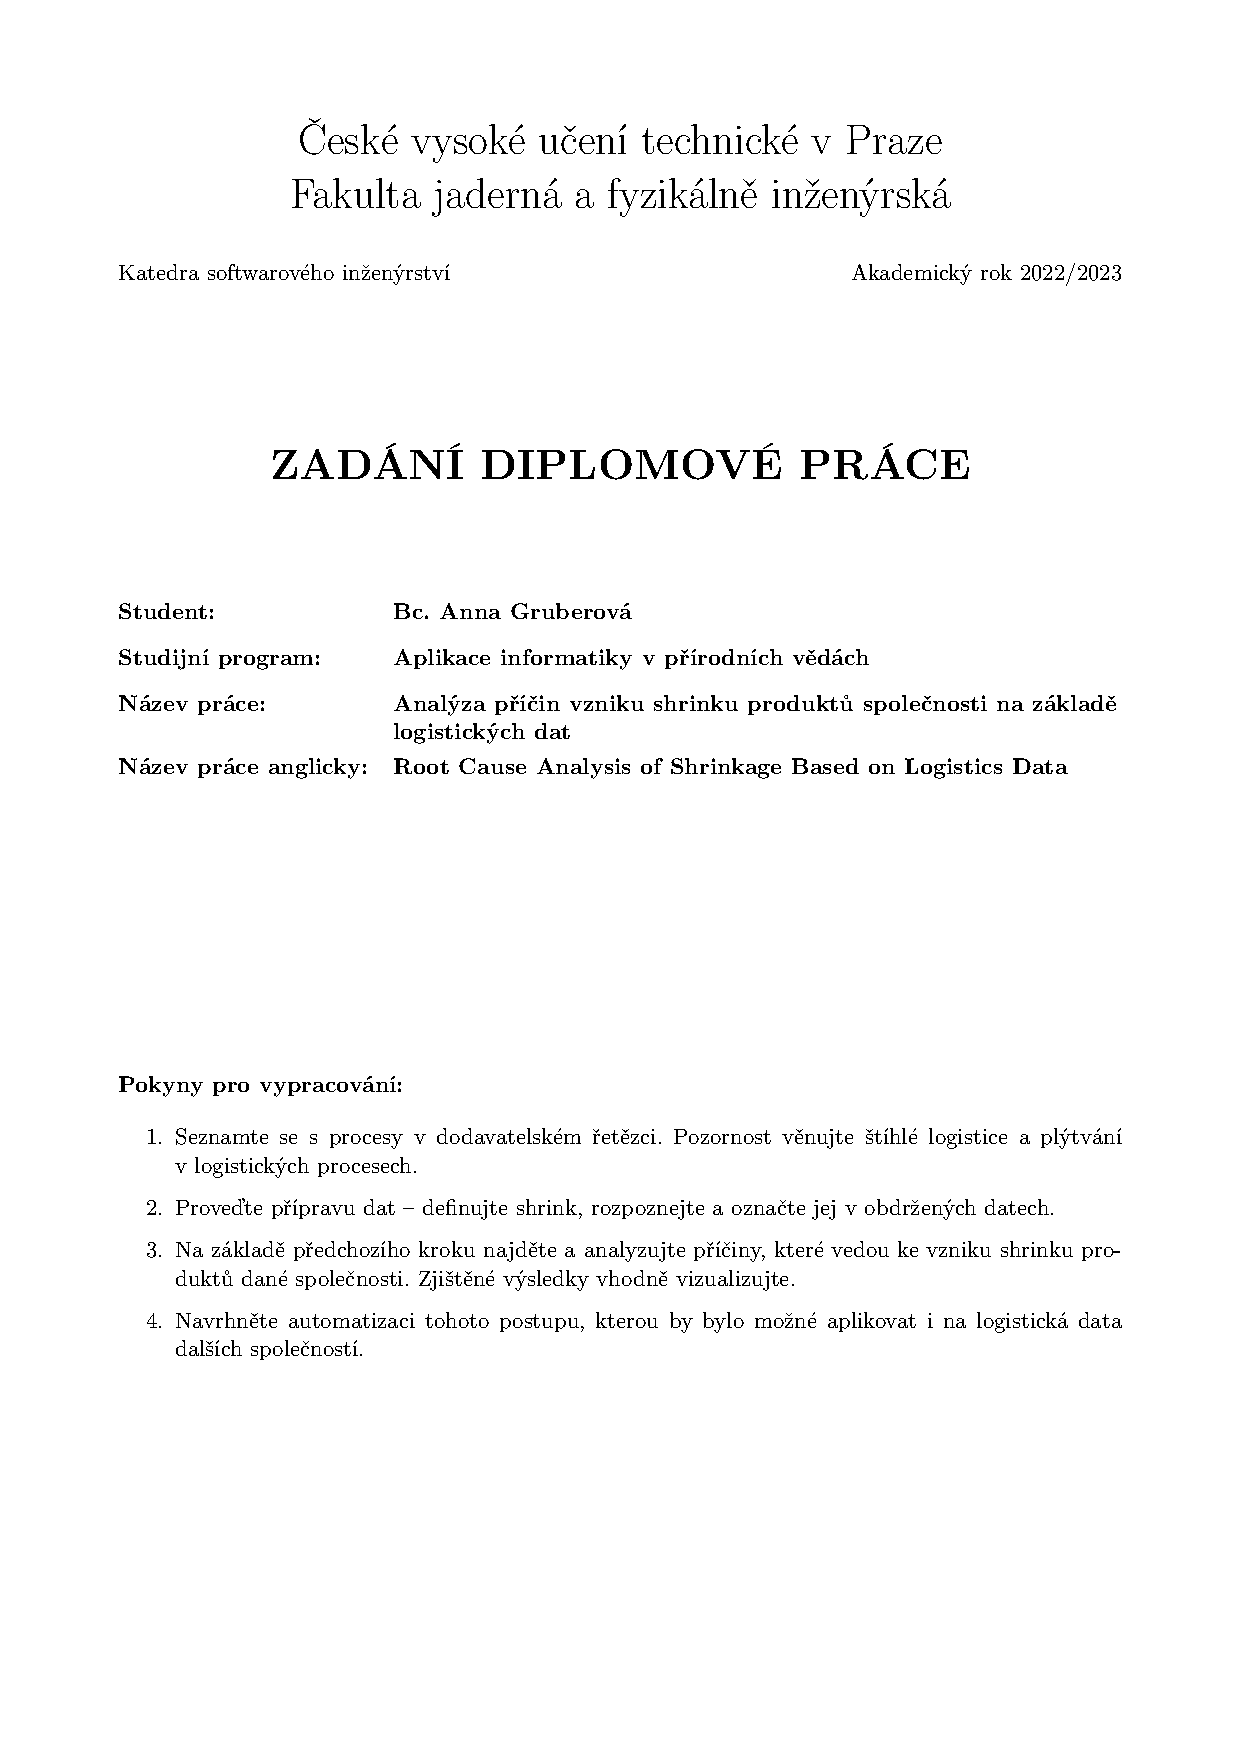
\includepdf[pages={1,2}]{zadaniDP.pdf} % NAHRAĎTE správným souborem!!!!DOPLNIT
%
%% --- varianta B: zadání naskenované jako jednotlivé stránky:
%\includepdf[pages={1}]{zadani1.pdf} % 1. strana zadání v PDF
%\includepdf[pages={1}]{zadani2.pdf} % 2. strana zadání v PDF
%
%% --- varianta C: zadání naskenované jako 2 samostatné obrázky:
%% 1. strana zadání
%\begin{center}
%     \includegraphics[width=1\textwidth]{zadani1.jpg}
%\end{center}
%% 2. strana zadání
%\newpage  % SEM NESAHEJTE!
%\thispagestyle{empty} % SEM NESAHEJTE!
%\begin{center}
%     \includegraphics[width=1\textwidth]{zadani2.jpg}zada
%\end{center}


%%%%%%%%%%%% Prohlášení -- SEM NESAHEJTE! Generuje se automaticky z výše nastavených maker \kde{} a \prohlaseni{}. %%%%%%%%%%%%
\newpage % SEM NESAHEJTE!
\thispagestyle{empty}  % SEM NESAHEJTE!

~ % SEM NESAHEJTE!
\vfill % prázdné místo. SEM NESAHEJTE!

\tb{Prohlášení} % SEM NESAHEJTE!

\vspace{1em} % vertikální mezera. SEM NESAHEJTE!
\prohlaseni

\vspace{2em}  % SEM NESAHEJTE!
\hspace{-0.5em}\begin{tabularx}{\textwidth}{X c}  % SEM NESAHEJTE!
V \kde\ dne .................... &........................................ \\	% SEM NESAHEJTE!
	& \autor
\end{tabularx}	% SEM NESAHEJTE!


%%%%%%%%%%%% Poděkování  %%%%%%%%%%%%
\newpage
\thispagestyle{empty}

~
\vfill % prázdné místo


% -- následující kus kódu (do "%%%%%%%%%%%% ABSTRAKT") můžete odstranit, pokud nechcete psát poděkování:
\tb{Poděkování}

\vspace{1em} % vertikální mezera
\podekovani
\begin{flushright}
\autor
\end{flushright}  % <------- tady končí stránka s poděkováním


%%%%%%%%%%%% ABSTRAKT atp. Je generován AUTOMATICKY podle maker nastavených na začátku souboru) %%%%%%%%%%%%
\newpage   % SEM NESAHEJTE!
\thispagestyle{empty}   % SEM NESAHEJTE!

% příprava:    (na následujících 8 řádků NESAHEJTE!)
\newbox\odstavecbox
\newlength\vyskaodstavce
\newcommand\odstavec[2]{%
    \setbox\odstavecbox=\hbox{%
         \parbox[t]{#1}{#2\vrule width 0pt depth 4pt}}%
    \global\vyskaodstavce=\dp\odstavecbox
    \box\odstavecbox}
\newcommand{\delka}{115mm} % šířka textů ve 2. sloupci tabulky

% použití přípravy:    % dovnitř "tabular" vůbec NESAHEJTE!
\begin{tabular}{ll}
  {\em Název práce:} & ~ \\
  \multicolumn{2}{l}{\bf \nazevcz} \\[1em]
  {\em Autor:} & \autor \\[1em]
  {\em Studijní program:} & \program \\
  {\em Obor:} & \obor \\
  {\em Druh práce:} & \druh \\[1em]
  {\em Vedoucí práce:} & \odstavec{\delka}{\vedouci\\ \pracovisteVed} \\
  {\em Konzultant:} & -- %\odstavec{\delka}{\konzultant \\ \pracovisteKonz}  % VYMAŽTE text "-- %" v případě, že jste neměli konzultanta
 \\[1em]
  \multicolumn{2}{l}{\odstavec{\textwidth}{{\em Abstrakt:} ~ \abstrCZ  }} \\[1em]
  {\em Klíčová slova:} & \odstavec{\delka}{\klicova} \\[2em]

  {\em Title:} & ~\\
  \multicolumn{2}{l}{\bf \nazeven}\\[1em]
  {\em Author:} & \autor \\[1em]
  \multicolumn{2}{l}{\odstavec{\textwidth}{{\em Abstract:} ~ \abstrEN  }} \\[1em]
  {\em Key words:} & \odstavec{\delka}{\keyword}
\end{tabular}



%%%%%%%%%%%% Obsah práce ... je generován AUTOMATICKY %%%%%%%%%%%%
\newpage  % SEM NESAHEJTE!
\parskip=0pt
\tableofcontents % SEM NESAHEJTE!
\parskip=7pt
\newpage % SEM NESAHEJTE!


%--------------------------------------------------------
%|         Zde začíná SAMOTNÁ PRÁCE (text)              |
%--------------------------------------------------------

\chapter*{Úvod} % SEM NESAHEJTE!
\addcontentsline{toc}{chapter}{Úvod} % SEM NESAHEJTE!
%
% %
% Tato diplomová práce se zabývá analýzou dat vybrané společnosti. Cílem práce je prozkoumat obdržená data, která se týkají tzv. shrinků. Jedná se o záznamy o produktech, které z~různých důvodů nemohly být prodány a kvůli tomu společnost přišla o zisk a vynaložila zbytečné náklady související s~nákupem a logistikou dotčených produktů. 

Na základě analýzy je třeba vyslovit hypotézy, které mohou souviset s~příčinou vzniku shrinku. Tyto hypotézy je třeba otestovat na datech a navrhnout tak možný postup pro hledání příčin existence shrinku produktů i v~datech dalších společností. 

% TODO

První kapitola se věnuje definici odborným pojmům z~logistiky, a to především z~odvětví, které se zabývá plýtváním. Popsány jsou tři hlavní typy plýtvání, dále jsou představeny možné zdroje plýtvání v~logistických procesech.

V následující kapitole se nachází teoretický popis metod, které jsem použila pro datovou analýzu. Jedná se o metody pro selekci příznaků a metodu GUHA. Dále jsou v~kapitole popsány důležité pojmy týkající se korelační analýzy. Závěr kapitoly je věnován popisu použitých nástrojů.

Ve třetí kapitole je definován pojem shrink a jeho klasifikace v~literatuře a v~obdrže-\\ných datech vybrané společnosti.

Další, čtvrtá kapitola popisuje způsob získání dat vybrané společnosti. Následuje popis jednotlivých databázových tabulek a jejich sloupců. Zbylá část kapitoly se zabývá přípravou vzorku pro další analýzy. Tedy kterou částí dat se zabývat na základě četnosti a metod pro selekci proměnných. Prozkoumány jsou vztahy mezi jednotlivými příznaky.

V páte kapitole je popsán business intelligence report vytvořený v~ aplikaci Power BI, který vizualizuje obdržená data. První část obsahuje popis jednotlivých stránek interaktivního reportu a popis použitých vizuálů. Druhá část je věnována závěrům, které z~reportu vyplývají.

Šestá kapitola obsahuje návrh řešení pro kategorizaci shrinkovaných produktů pomocí korelační analýzy. V~kapitole je uveden postup analýzy a popis implementace v~jazyce Python. Konec kapitoly je věnován ukázce výsledků této metody.

Poslední kapitola analyzuje data pomocí procedury GUHA a metody 4ftMiner. V~této kapitole bylo vysloveno několik hypotéz a následně byla ověřována jejich platnost.



% - Data
%     - jak jsou data uložená v~DB u zákazníka
%         - provázané
%     - SQL příkazy
%     - výběr proměnných
%     - target hodnoty - cost, množství
%     - produktová Hierarchie
% - Vymazaní outlierů
%     - outlier metody
%     - businessově

% - Co vysvetluje target
%     - Miner
%     - PCA

% - Korelační analýza mezi produkty v~rámci kategorie
%     - korelace 
% - Rozčlenění produktů

% - Vizualizace dat
%     - Jak funguje PBI
%     - Seznam metri
Tato diplomová práce se zabývá analýzou dat vybrané společnosti. Cílem práce je prozkoumat obdržená data, která se týkají tzv. shrinků. Jedná se o záznamy o produktech, které z~různých důvodů nemohly být prodány a kvůli tomu společnost přišla o zisk a vynaložila zbytečné náklady související s~nákupem a logistikou dotčených produktů. 

Na základě analýzy je třeba vyslovit hypotézy, které mohou souviset s~příčinou vzniku shrinku. Tyto hypotézy je třeba otestovat na datech a navrhnout tak možný postup pro hledání příčin existence shrinku produktů i v~datech dalších společností. 

% TODO

První kapitola se věnuje definici odborným pojmům z~logistiky, a to především z~odvětví, které se zabývá plýtváním. Popsány jsou tři hlavní typy plýtvání, dále jsou představeny možné zdroje plýtvání v~logistických procesech.

V následující kapitole se nachází teoretický popis metod, které jsem použila pro datovou analýzu. Jedná se o metody pro selekci příznaků a metodu GUHA. Dále jsou v~kapitole popsány důležité pojmy týkající se korelační analýzy. Závěr kapitoly je věnován popisu použitých nástrojů.

Ve třetí kapitole je definován pojem shrink a jeho klasifikace v~literatuře a v~obdrže-\\ných datech vybrané společnosti.

Další, čtvrtá kapitola popisuje způsob získání dat vybrané společnosti. Následuje popis jednotlivých databázových tabulek a jejich sloupců. Zbylá část kapitoly se zabývá přípravou vzorku pro další analýzy. Tedy kterou částí dat se zabývat na základě četnosti a metod pro selekci proměnných. Prozkoumány jsou vztahy mezi jednotlivými příznaky.

V páte kapitole je popsán business intelligence report vytvořený v~ aplikaci Power BI, který vizualizuje obdržená data. První část obsahuje popis jednotlivých stránek interaktivního reportu a popis použitých vizuálů. Druhá část je věnována závěrům, které z~reportu vyplývají.

Šestá kapitola obsahuje návrh řešení pro kategorizaci shrinkovaných produktů pomocí korelační analýzy. V~kapitole je uveden postup analýzy a popis implementace v~jazyce Python. Konec kapitoly je věnován ukázce výsledků této metody.

Poslední kapitola analyzuje data pomocí procedury GUHA a metody 4ftMiner. V~této kapitole bylo vysloveno několik hypotéz a následně byla ověřována jejich platnost.



% - Data
%     - jak jsou data uložená v~DB u zákazníka
%         - provázané
%     - SQL příkazy
%     - výběr proměnných
%     - target hodnoty - cost, množství
%     - produktová Hierarchie
% - Vymazaní outlierů
%     - outlier metody
%     - businessově

% - Co vysvetluje target
%     - Miner
%     - PCA

% - Korelační analýza mezi produkty v~rámci kategorie
%     - korelace 
% - Rozčlenění produktů

% - Vizualizace dat
%     - Jak funguje PBI
%     - Seznam metri

\chapter{}

\cite{bib:Jones}

\section{Logistika}

\subsection*{Definice Logistiky}

Logistika zahrnuje všechny operace, které se týkají doručení zboží nebo služeb od výrobce k zákazníkovi, s výjimkou samotné výroby zboží nebo provádění služby. Výrobou je naopak rozuměno vše, co mění podobu materiálu.
Během výroby se však logistika uplatňuje, například jako přesun materiálu nebo polotovarů mezi jednotlivými výrobními zařízeními. 
% Obdobně při poskytování služby je podstatné se zabývat 
Operace lze rozdělit do tří hlavních toků: materiálový, informační a finanční tok. Materiálový obsahuje všechny pohyby týkající se fyzického materiálu, tedy jeho získávání, přesuny a skladování, a to jak mezi zákazníky, dodavateli či výrobními areály a sklady, tak i vnitřní pohyby mezi produkčními linkami nebo skladovými pozicemi. Informační tok popisuje procesy vznikající během materiálového toku, dále se do něj řadí analýzy již proběhlých toků a plánování a předpovědi budoucích toků. Poslední kategorie, finanční tok mapuje náklady způsobené předešlými dvěma zmíněnými toky.\cite{bib:Baudin}

Pojem logistika je úzce propojen s pojmem Supply Chain Management (SCM)\footnote{Do češtiny lze Supply Chain Management přeložit jako řízení či správa dodavatelského řetězce. V českém prostředí se používá jak anglická tak česká podoba.}. Zatímco logistika se zabývá toky zboží, služeb či lidí, Supply Chain Management zahrnuje operace logistiky, navíc ale sleduje vztahy mezi procesory, které koordinuje a optimalizuje za účelem naplnění určitých cílů. Tímto cílem bývá často snížení nákladů v rámci částí procesu nebo zvýšení konkurenceschopnosti podniku \cite{bib:IIMudaipur}. Supply Chain Management se tedy prolíná s pojmem logistika a bývají často zaměňovány. Důvodem může být i to, že se jedná o nový pojem, který byl poprvé použitý v roce 1982.\cite{bib:Christopher} 

\section{Štíhlá logistika}

Rozdělení 

\subsection*{MUDA}
\subsection*{MULA}
\chapter{Použité metody}

První část této kapitoly se věnuje teoretickému popisu použitých metod v~této práci. Nejprve jsou
% korelace
% ortogonální
% kontingencni tabulka (vicenasobna)

% zkrtky PCA, MCA, CA,
% znaceni jednotkový vektor rozměru J \mathbf{1}_J
% Singulární rozklad (zkratkou SVD podle anglického názvu Singular Value Decomposition) matice + singulární hodnoty


\section{Redukce dimenzionality} %Extrakce proměnných}

\subsection{Analýza hlavních komponent}

Analýza hlavních komponent (anglicky \emph{Principal component analysis}, dále jako PCA) je statistická metoda využívaná pro pro extrakci proměnných, redukci vícedimenzio-\\nálních dat nebo vizualizaci dat. Lze ji aplikovat pouze na kvantitativní data s~numerickými, spojitými hodnotami, neboť metoda využívá lineární algebraické techniky, jako je například kovarianční matice, pro jejíž výpočet se předpokládají spojité hodnoty. 

Jednotlivá pozorování obsažená v~datech bývají popsána několika různými příznaky. Tyto příznaky jsou často vzájemně korelované a obsahují šum. Metoda PCA dovede extrahovat pouze důležité informace z~proměnných a snížit šum. K~tomu je třeba vypočítat nové ortogonální proměnné, nazývané hlavní komponenty, které se získají jako lineární kombinace původních proměnných \cite{bib:PCA1}. Hlavní komponenty reprezentují směry největšího rozptylu původních dat a jsou řazeny podle své významnosti. Jinými slovy, první hlavní komponenta zachycuje co nejvíce variability v~datech, druhá hlavní komponenta zachycuje co nejvíce variability, která nebyla zachycena první hlavní komponentou, pro zbylé komponenty analogicky. \cite{bib:PCA3}
%, jinými slovy se jedná o přímku,  které nesou největší informaci o datech. Hlavní komponentu si lze představit jako novou osu, která umožňuje vidět data v~takovém rozložení, že rozdíly mezi pozorováními jsou lépe patrné.  %https://builtin.com/data-science/step-step-explanation-principal-component-analysis

\subsubsection{Princip}

Předpokládáme množinu dat $\mathbf{X} = (\bm{x}_1, \ldots, \bm{x}_N )$, kde $N$ j počet pozorování a každý vektor $\bm{x}_i$ přísluší jednomu pozorování popsanému $M$ proměnnými. $\mathbf{X}$ je potom matice rozměru $N\times M$ vstupních dat. Dále je definovaný výběrový průměr $\bar{\bm{x}}$ jako
\begin{equation}
    \bar{\bm{x}} = \frac{1}{N} \sum_{i=1}^{N} \bm{x}_i,
\end{equation}
a výběrová kovarianční matice $\mathbf{C}$

\begin{equation}
    \mathbf{\mathbf{C}} = \frac{1}{N} \sum_{i=1}^{N} (\bm{x}_i - \bar{\bm{x}}).
\end{equation}

První hlavní komponentu, která popisuje největší rozptyl dat označíme $y_{1i}$ a vypočte-\\me následovně jako lineární kombinaci původních proměnných
\begin{equation}
    y_{1i} = \bm{a}_1^\top (\bm{x}_i - \bar{\bm{x}}), \quad \mbox{pro } i=1,\ldots,N,
\end{equation}
kde $\bm{a}_1 = (a_{11}, \ldots, a_{M1})^\top $ je vektor vah. 

Optimální vektor $\bm{a}_1$ je takový vektor, který maximalizuje výběrový rozptyl nové proměnné $y_{1i}$ za podmínky $\bm{a}_1^\top\bm{a}_1 = 1$. Pakliže je výběrový rozptyl $y_{1i}$ definován jako 
\begin{equation}
    D(y_{11}, \ldots, y_{1N}) = \bm{a}_1^\top \mathbf{C} \bm{a}_1
\end{equation}
můžeme maximalizační úlohu vyřešit pomocí metody Lagrangeových multiplikátorů. Lagrangeova funkce s~parametrem $\lambda_1$ má následující tvar
\begin{equation}
    \mathcal{L}(\bm{a}_1, \lambda_1) = \bm{a}_1^\top \mathbf{C} \bm{a}_1 - \lambda_1(\bm{a}_1^\top\bm{a}_1 - 1).
\end{equation}

Derivaci funkce položíme rovnou nule 
\begin{align*}
    \frac{\partial \mathcal{L}}{\partial \bm{a}_1}  = 2 \mathbf{C} \bm{a} - 2\lambda_1 \bm{a}_1 \overset{!}{=}  0 \\
    (\mathbf{C} - \lambda_1 \mathbf{I} ) \bm{a}_1 \overset{!}{=}  0,  \\
\end{align*}
kde $\mathbf{I}$ je jednotková matice.

Řešíme soustavu lineárních rovnic pro neznámý parametr $\bm{a}_1$, která má řešení právě tehdy, když je matice $\mathbf{C} - \lambda_1 \mathbf{I} $ singulární, tedy platí, že její determinant  je roven nule. $\lambda_1$ je pak největší vlastní číslo matice $\mathbf{C}$ a $\bm{a}_1$ vlastní vektor příslušný tomuto vlastnímu číslu. Toto tvrzení se matematicky zapíše následovně
\begin{equation}
    \mathbf{C} \bm{a}_1 = \lambda_1 \bm{a}_1. \\
\end{equation}
Po vynásobení vektorem $\bm{a}_1$ zleva získáme řešení pro maximální rozptyl proměnné $y_{1i}$
\begin{equation}
    D(y_{11}, \ldots, y_{1N}) = \bm{a}_1^\top \mathbf{C} \bm{a}_1 = \lambda_1.
\end{equation}


Druhá hlavní komponenta
\begin{equation}
    y_{2i} = \bm{a}_2^\top (\bm{x}_i - \bar{\bm{x}}), \quad \mbox{pro } i=1,\ldots,N,
\end{equation}
se vypočte obdobným způsobem s~přidanou podmínkou ortogonality vzhledem k~první hlavní komponentě -- druhá hlavní komponenta nesmí být korelovaná s~před-\\chozí, první hlavní komponentou. Potom popisuje druhý největší možný rozptyl v~datech. Znázornění dvou hlavních komponent ve dvoudimenzionálním prostoru je vyobrazeno na obrázku \ref*{obr:met:PCA1}.
Vektor  $\bm{a}_2$ se opět získá jako jednotkový vlastní vektor kovarianční matice $\mathbf{C}$ příslušící druhému největšímu vlastnímu číslu $\lambda_2$.\cite{bib:PCA1, bib:PCA3} %https://builtin.com/data-science/step-step-explanation-principal-component-analysis

\begin{figure}[hbtp!]
    \centering
    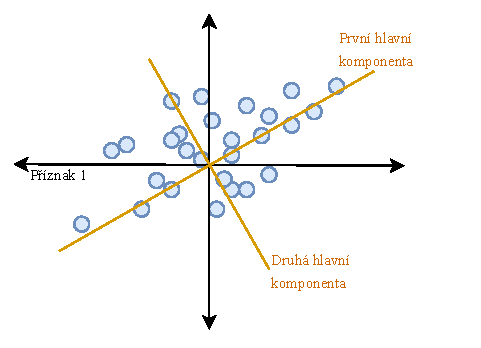
\includegraphics[width=0.7\textwidth]{obrazky/PCA.pdf}
    \caption{Znázornění dvou hlavních komponent na pro dvě proměnné. Zdroj: vlastní.}
    \label{obr:met:PCA1}
\end{figure}

Získání předpisů pro další hlavní komponenty je analogické. Obecně lze zapsat metodu PCA a převod původních proměnných následujícím maticovým zápisem
\begin{equation}
    \mathbf{Y} = \mathbf{XA}, 
\end{equation}
kde $\mathbf{Y}$ obsahuje komponenty $\bm{y}_{1}, \bm{y}_{2}, \ldots$, $\mathbf{X}$ je matice vstupních dat, $\mathbf{A}$ je matice vlastních vektorů kovarianční matice $\mathbf{C}$. Pro matici $\mathbf{A}$ zároveň platí $\mathbf{C} =  \mathbf{A} \mathbf{\Lambda} \mathbf{A}^\top$, kde $\mathbf{\Lambda}$ je diagonální matice vlastních čísel $\mathbf{C}$.\cite{bib:PCA2}

\subsection{Korespondenční analýza}

Vícenásobná korespondenční analýza (anglicky \emph{Multiple correspondence analysis}, dále jako MCA) je metoda, která umožňuje popsat vztahy mezi daty, které jsou popsané kategorickými proměnnými, vytvořením kontingenční tabulky. V~případě, že se popisuje vzájemná relace pouze dvou proměnných, se použije základní korespondenční analýza\footnote{anglicky \emph{correspondence analysis} (CA)}. MCA je alternativou~k PCA, pokud jsou analyzovanými daty kategorická data. \cite{bib:MCA1}

% \subsubsection{Princip korespondenční analýzy}
\subsubsection{Značení}
%https://statmath.wu.ac.at/courses/CAandRelMeth/caipA.pdf
Nechť $\mathbf{N}$ je matice dat s~rozměry $I\times J$, kde I odpovídá počtu pozorování a J je počet kategorií. %asi pocet kategorii, najit !!!
Matice $\mathbf{N}$ je převedena na korespondenční matici $\mathbf{P}$ vydělením matice $\mathbf{N}$ jejím celkovým součtem $n = \sum_{i=1}^{I} \sum_{j=1}^{J} n_{ij}=\mathbf{1}^\top_I \mathbf{N}\mathbf{1}_J$. To zaručuje, že součet prvků matice $\mathbf{P}$ je roven jedné. Tyto kroky lze shrnout následujícím matematickým zápisem
\begin{equation}
    \mathbf{P} = \frac{1}{n}\mathbf{N}, \qquad \mathbf{P} = \{p_{ij}\},  \qquad  \sum_{i=1}^{I} \sum_{j=1}^{J} p_{ij} = 1.
\end{equation}
Součet $i$tého řádku, resp. součet $j$tého sloupce je značen následovně
\begin{align*}
    r_i = \sum_{j=1}^{J} \qquad \mbox{ pro } i=1,\ldots,I, \\
    c_j = \sum_{i=1}^{I} \qquad \mbox{ pro } j=1,\ldots,J.
\end{align*}
Vektor $\bm{r} = \mathbf{P} \mathbf{1}_J $ obsahuje všechny řádkové součty matice $\mathbf{P}$, analogicky vektor $\bm{c} = \mathbf{P}^\top \mathbf{1}_I $ obsahuje všechny sloupcové součty téže matice.

Pro další výpočty zavedeme značení pro diagonální matice, které mají na diagonále  řádkový, resp. sloupcový součet
\begin{equation}
    \mathbf{D}_r = \mbox{diag}(\bm{r}), \quad \mbox{ resp. } \quad \mathbf{D}_c = \mbox{diag}(\bm{c}).
\end{equation}

% Pro připomenutí je vhodné dodat, že součet matice P je jedna

\subsubsection[Výpočetní algoritmus základní korespondeční analýzy]{Výpočetní algoritmus základní korespondeční analýzy \cite{bib:CA1,bib:MCA2}}
Označme $\mathbf{S}  = \{s_{ij}\}$ následující matici
\begin{equation}
    \mathbf{S} := \mathbf{D}_r^{-\frac{1}{2}} (\mathbf{P} - \bm{rc}^\top) \mathbf{D}_c^{-\frac{1}{2}}.
\end{equation}
Po té proveďme singulární rozklad této matice
\begin{equation}
    \mathbf{S} = \mathbf{U}\mathbf{\Delta}\mathbf{V}^\top,
\end{equation}
kde $\mathbf{\Lambda} = \mathbf{\Delta}^2$ je matice vlastních čísel $\lambda_k$ pro $k=1,\ldots,K$, kde $K=min\{I-1,J-1\}$. Potom rozměry matice $\mathbf{U}$, resp. $\mathbf{V}$ jsou $I\times k$, resp.  $J\times k$. Dále platí $\mathbf{U}^\top\mathbf{U}=\mathbf{V}^\top\mathbf{V}=\mathbf{I}$.%https://www.wikiwand.com/en/Correspondence_analysis


% Zatímco u PCA je měřítkem úspěchu míra rozptylu popsaná prvními vybranými hlavními komponentami 
Korespondenční analýza měří míru váženého rozptylu, tzv. inercii pomocí vlastních čísel $\lambda_k$ matice $\mathbf{S}$, $\lambda_k$ se pak nazývají hlavní inercie.
Celková inercie je rovna
\begin{equation}
    I = \sum_{k=1}^{K} \lambda_k = \sum_{i=1}^{I}\sum_{j=1}^{J} s_{ij}^2.
\end{equation}

Hlavní komponenta řádků $\mathbf{F}$ je rovna
\begin{equation}
    \mathbf{F} = \mathbf{D}_r^{-\frac{1}{2}} \mathbf{U}  \mathbf{\Delta}.
\end{equation}
Hlavní komponenta sloupců $\mathbf{G}$ je rovna
\begin{equation}
    \mathbf{G} = \mathbf{D}_c^{-\frac{1}{2}} \mathbf{V}  \mathbf{\Delta}
\end{equation}

\subsubsection*{Výpočetní algoritmus MCA}

Předpokládejme, že původní matice kategorických dat má tvar $N\times Q$, tj. $N$ pozorování a $Q$ proměnných. Matici dat převedeme na indikátorovou matici. Indikátorová matice  $\mathbf{Z} $ je vytvořena tak, že kategorická data jsou rozepsána do pomocných pro-\\měnných. Pokud $q$tá proměnná má $J_q$ typů kategorií, tak příslušná indikátorová matice bude mít $J = \sum_{q=1}^{Q}J_q$ sloupců a $N$. Tzn. počet proměnných byl tímto rozepsáním rozšířen z~počtu původních $Q$ proměnných na $J$ proměnných.
% Klasická MCA má dvě podoby.
První způsob MCA aplikuje základní algoritmus korespondenční analýzy na matici  $\mathbf{Z}$, takto se získají souřadnice pro $N$ pozorování a $J$ kategorií.

% https://towardsdatascience.com/famd-how-to-generalize-pca-to-categorical-and-numerical-data-2ddbeb2b9210 
% https://arrow.tudublin.ie/cgi/viewcontent.cgi?article=1227&context=scschcomdis

% \subsection{Particle Swarm Optimization}

% https://www.analyticsvidhya.com/blog/2021/10/an-introduction-to-particle-swarm-optimization-algorithm/

\section{Korelační analýza}
\label{sec:Teoriekorelace}
\subsection{Korelační koeficient}

Pojem korelace obecně znamená vzájemný vztah mezi dvěma veličinami. Pokud se jedna veličina mění, pak se mění dle míry korelace i druhá veličina. Samotná korelace ale neurčuje míru vztahu, ani směr vztahu. Tedy která veličina je příčinou a která důsledkem. Tuto vlastnost popisuje kauzalita. Míra korelace mezi dvěma veličinami je určena pomocí korelačního koeficientu. Existuje více způsobů měření míry korelace, v~následující části jsou popsány vybrané z~nich.\cite{bib:MB}

Nejčastěji používaným koeficientem pro měření korelace je \emph{Pearsonův korelační koeficient}. Nechť $X$ a $Y$ jsou náhodné veličiny s~realizacemi $x_1, x_2, \ldots$ a $y_1, y_2, \ldots$, potom hodnota Pearsonova koeficientu se vypočítá jako:
\begin{equation}
    r_p = \frac{\mathrm{cov}(X,Y)}{\sigma_X\sigma_Y} = 
    \frac{ \sum_{i=1}^{n}(x_i-\bar{x})(y_i-\bar{y}) }
    {
        \sqrt{
            \sum_{i=1}^{n}(x_i-\bar{x})^2
            \sum_{i=1}^{n}(y_i-\bar{y})^2
            }
    } 
    = \frac{ \sum_{i=1}^{n}x_i y_i - n\bar{x}\bar{y} }
    {
          (n-1) s_{x} s_{y}
    }
\end{equation}
kde $\bar{x}, \bar{y}$ jsou výběrové průměry, $s_x, s_y$ výběrové směrodatné odchylky.\cite{bib:MB}

Tento koeficient měří lineární vztah mezi dvěma proměnnými. Hodnoty se pohybují v~intervalu $\langle -1, 1 \rangle$. Krajní hodnoty znamenají dokonalou lineární závislost. Pokud je koeficient roven 1, pak pokud roste jedna veličina, roste i hodnota druhé veličiny. Pokud je koeficient roven -1, potom s~rostoucí hodnotu jedné veličiny, klesá hodnota druhé. Zatímco je-li hodnota koeficientu rovna nule, veličiny jsou lineárně zcela nekorelované. Pro výpočet totoho koeficientu je předpokládána normalita zkoumaných dat.\cite{bib:MB}

Další koeficient, který měří korelaci mezi dvěma veličinami, je \emph{Spearmanův korelační koeficient}. Tento neparametrický koeficient měří nelineární závislost dvou veličin, určuje, jak moc jejich vztah odpovídá monotónní funkci. Spearmanův koeficient je robustní vůči odlehlým hodnotám a nevyžaduje normalitu dat, protože pracuje se seřazenými hodnotami obou veličin. Hodnoty opět leží mezi $-1$ a $1$ a platí pro mě analogická tvrzení jako Pearsonův korelační koeficient.\cite{bib:MB,bib:correlation}

Nechť $X$ a $Y$ jsou náhodné veličiny s~realizacemi $x_1, x_2, \ldots$ a $y_1, y_2, \ldots$ a číslo $x_{ri}$ je pořadí čísla $x_i$ v~rámci všech hodnot veličiny $X$, číslo $y_{ri}$ je pořadí čísla $y_i$ v~rámci všech hodnot veličiny $Y$. $\bar{x}_r, \bar{y}_r$ jsou průměrná pořadí a $s_{x_r}, s_{y_r}$ příslušné směrodatné odchylky. Vztah pro výpočet Spearmanova koeficientu je:
\begin{equation}
    r_s =
    \frac{ \sum_{i=1}^{n}x_iy_i - n\bar{x}_r\bar{y}_r }
    {
          (n-1) s_{x_r} s_{y_r}
    }.
\end{equation}
Pokud předpokládáme, že pořadí hodnot je unikátní, tj. neexistují v~rámci jedné veličiny hodnoty realizace se stejnou hodnotou, pak lze vzorec pro výpočet Spearmanova korelačního koeficientu zjednodušit na:
\begin{equation}
    r_s = 1-
    \frac{ 6 \sum_{i=1}^{n}d_i^2 }{n(n^2-1)},
\end{equation}
kde $d_i = (x_{ri} - y_{ri})$ je diference pořadí hodnot veličin $X$ a $Y$.\cite{bib:MB,bib:correlation}

Jak je patrné ze vzorců pro oba korelační koeficienty tato míra lze aplikovat pouze na numerické veličiny. V~případě kategorických veličin by bylo potřeba je převést na číselné hodnoty. K~tomu slouží řada metod. Mezi dva nejznámější způsoby překódo-\\vání kategorických proměných patří one-hot kódování a label kódování. V~případě one-hot kódování se ale může počet proměnných výrazně zvýšit, pokud v~datech existují příznaky s~větším počtem unikátních kategorií. Pro druhý zmíněný způsob kódování je nevýhodou fakt, že přiřazením čísel od 0 do $n$, kde $n$ je počet kategorií v~příznaků, se kategorickým hodnotám přiřadí pořadí, které ale v~datech vůbec nemusí být a tudíž je tato nová informace v~datech na obtíž. Další možností je předělat kategorické hodnoty na spojité hodnoty pomocí cílového sloupec (tj. vysvětlované proměnné), tímto způsobem ale může dojít k~zanesení informace o předpovídaném sloupci přímo do vysvětlujících proměnných. \cite{bib:encoding}. Proto jsou v~další části této sekce uvedeny vybrané způsoby měření závislosti dvou kategorických proměnných.

\subsection{Další způsoby měření závislosti}

Pro měření míry závislosti dvou kategorických proměnných lze použít \emph{Cramerovo V}, dále značeno jako $V$. 
Hodnota koeficientu se pohybuje mezi 0 a 1. 1 znamená dokonalou závislost mezi proměnnými, 0 neznamená žádnou závislost. Tento koeficient nemůže nabýt negativní hodnoty, tj. neexistuje negativní závislost. Stejně jako předchozí koeficienty pro korelaci je $V$ symetrické a nezáleží na pořadí veličin.\cite{bib:correl,bib:MB}

Pro dvě zkoumané veličin $X, Y$ s~hodnotami $x_1, x_2, \ldots, x_r$ a $y_1, y_2, \ldots, y_s$ existuje kontingenční tabulka $\mathbf{K}$ těchto veličin, jejíž prvky jsou četnosti hodnot proměnných $n_{ij}$,tj. kdy byly pozorovány hodnoty pro dvojici $(x_i, y_j)$. $r$, resp. $s$ je počet řádků, resp. sloupců kontingenční tabulky $\mathbf{K}$.
Vzorec pro Cramerovo $V$ má tvar:
\begin{equation}
    V~= \sqrt{\frac{\chi^2 / n}{min(r-1, s-1)}},
\end{equation}
kde statistika $\chi^2$ se výpočítá následovně
\begin{equation}
    \chi^2 = \sum_{i=1}^n \frac{(n_ij - n_in_j/n)^2}{n_in_j/n},
\end{equation}
kde $n_i$ je četnost výskytu hodnoty $x_i$, $n_j$ je četnost výskytu hodnoty $y_j$. Tedy platí $n_i=\sum_{i=0}^r{n_{ij}}$ a $n_j=\sum_{j=0}^s{n_{ij}}$.\cite{bib:statology,bib:correl,bib:MB}

Pro určení kolik informace o jedné proměnné nese druhá proměnná, je popsáno
pomocí \emph{ vzájemné informace} \cite{bib:MI}. Informací lze rozumět obsah jakéhokoli oznámení nebo údaje, který se přenáší v~daném čase a prostoru. Podle Shannona, zakladatele teorie informace, je informace míra množství neurčitosti nebo nejistoty o nějakém náhodném jevu, která se odstraní realizací daného jevu \cite{bib:MI2}. Informací tak může být stanovení výsledku náhodného jevu, tedy se jedná o hodnotu náhodné veličiny \cite{bib:MI}. Pro definování vzájemné informace je třeba definovat ještě \emph{vlastní informace} a pojem \emph{entropie}.

Dále jsou sepsány předpoklady pro výpočet množství informace. Pokud má náhodný jev $X$ $n$ realizací, pak je množství informace funkcí $n$. Pakliže je $n=1$, množství informace se rovná nule, neboť se jedná o jev jistý. 
Pokud jevy $X$ A $Y$ probíhají nezávisle, ale ve stejný čas, tj. $p_{XY}(x,y)=p_X(x)\cdot p_Y(y)$, potom množství informace obou jevů se tovná součtu jejich množství.
Pokud jev $X$ má $n $ realizací a jev $Y$ $m$ realizací, kde $m>n$, potom se očekává, že množství informace jevu $Y$ je větší než množství in
formace jevu $X$. \cite{bib:MI2} Pokud je pravděpodobnost každé realizace stejná, tj. $p_X(x) = 1/n$, pak  Hartleyho míra informace je definována jako funkce $I: \mathbf{N} \leftarrow \mathbf{R}$ ve tvaru $I(n)=\log n$. Pro vlastní míru informace obsažené ve výsledku $x$ pak platí: \cite{bib:MI2, bib:MI3}
 \begin{equation}
    I(x)=- \log p_{X}(x).
 \end{equation}

Množství informace celého jevu je popsáno entropií náhodné veličiny. Entropie $H(X)$ náhodné veličiny $X$ s~hodnotami $x_1, x_2, \ldots $ s~pravděpodobnostní funkcí $p(x)$ je rovna: \cite{bib:MI2,bib:literatura}
 \begin{equation}
    H(X) = -\sum_x p_{X}(x) \log p_{X}(x).
 \end{equation}

Nechť je dán vektor $(X,Y)$, kde $X$, resp. $Y$ je náhodná veličina nabývající hodnot $x_1, x_2, \ldots $, resp. $y_1, y_2, \ldots$. Náhodný vektor nabývá hodnot $(x_1, y_1), (x_2, y_2), \ldots $. Sdružená entropie vektoru  $(X,Y)$ má tvar: \cite{bib:MI,bib:MI3}
\begin{equation}
    H(X,Y) = -\sum_{(x,y)} p_{XY}(x,y) \log p_{XY}(x,y).
 \end{equation}
Podmíněná entropie s~předpokladem $p_Y(y)>0$: \cite{bib:MI3}
\begin{equation}
    H(X|Y=y) = -\sum_{(x,y)} p_{X|Y}(x|y) \log p_{X|Y}(x|y),
    \label{eq:podmEntropie}
 \end{equation}
kde podmíněná pravděpodobnost je rovna $p_{X|Y}(x|y) = p_{XY}(x,y) / P_Y(y)$.

Pokles entropie se měří pomocí vzájemné informace, tj. platí věta \cite{bib:MI3}:
\begin{equation}
    I(X;Y) = -H(X,Y)+H(X)+H(Y).
 \end{equation}

Vzájemná informace měří ztrátu informace v~důsledku závislosti $X$ a $Y$. Jinými slovy, kolik informace o jedné proměnné $X$ nese druhá proměnná $Y$. Matematicky je vzájemná informace definována následovně: \cite{bib:MI, bib:MI3, bib:literatura}
\begin{equation}
    I(X;Y) = \sum_{(x,y)} + \log \frac{p_{X\vert Y}(x\vert y)}{p_X(x)}
\end{equation}

Míra, která dovede změřit asymetrickou závislost kategorických proměnných se nazý-//vá \emph{Thielovo U}, které se někdy označuje jako koeficient nejistoty. Pro jeho výpočet se používá podmíněná entropie, viz vztah \ref{eq:podmEntropie}. Thielovo $U$  nabývá hodnot z~intervalu $\langle 0, 1 \rangle$, kde 0 neznamená žádnou závislost a 1 dokonalou závislost. Hodnota není symetrická, tj. $U(X,Y)\neq U(Y,X)$, proto se může používat značení, které určuje směr závislosti -- $U(X,Y) = U(X|Y)$. Vzorec pro výpočet koeficientu $U$ je: \cite{bib:thiel,bib:correl}
\begin{equation}
    U(X,Y) = U(X|Y) = \frac{H(X)-H(X-Y)}{H(X)}.
\end{equation}

\section*{Ostatní použité pojmy}

Při analýze dat lze narazit na problém multikolinearity. \emph{Multikolinearita} je vzájemná lineární závislost vysvětlujících proměnných. Jeli $\mathbf{A}$ matice dat (vysvětlujících pro-\\měnných bez předpovídaného sloupce), pak multikolinearita v~datech existuje, pokud platí rovnice pro alespoň jedno nenulové $c_i$: $c_1\bm{a}_1 + ... + c_k\bm{a}_k$, kde $c_i$ jsou konstanty a $\bm{a}_i$ sloupce matice reprezentující jednotlivé příznaky, $k$ počet sloupců matice, tj. počet příznaků. V~reálných datech stačí, když je daná rovnice přibližně splněna.\cite{bib:MB}

Měřítkem multikolinearity je \emph{rozptylový inflační faktor} (zkratka VIF z~anglického variance inflation factor). Možné hodnoty pro koeficient jsou 1 až libovolné číslo větší než jedna, 1 znamená nezávislost. Nad určitou hodnotu koeficientu, v~literatuře \cite{bib:multi} je uvedeno už číslo větší než 5, je značná multikolinearita již přítomna v~datech. Koeficient má pro $i$-tý sloupec matice $\mathbf{A}$ tvar:
\begin{equation}
    VIF_i = \frac{1}{1-R_i^2},
\end{equation}
kde $R_i^2$ je koeficient determinace $i$-tého sloupce. Ten říká, jak velkou část variability závislé proměnné je možné vysvětlit.\cite{bib:multi}

\section{Metoda GUHA}
\label{sec:Teorie:Guha}

Metoda GUHA je původní česká metoda používaná pro neexplorační analýzu dat.
První článek o této metodě vyšel v~roce 1966. V~současné době je jedním z nejrozsáhlejších implementací metody systém LISp-Miner. Jedná se o software vyvíjený na Fakultě informatiky a statistiky Vysoké školy ekonomické v~Praze, kde se zároveň používá pro výuku a výzkum dobývaní znalostí z~databází \cite{bib:GUHA}. Zároveň je také implementována knihovna \emph{CleverMiner} v~jazyce Python, která disponuje částí funkcionalit softwaru LISp-Miner.

\subsection{Základní princip metody}

Cílem metody GUHA je získat z~pozorovaných dat všechny vztahy, které jsou jsou pravdivé pro množinu objektů, ze které pochází zkoumaná data. Využívají se k~tomu statistické testy hypotéz, které dovolují na základě platnosti určitého tvrzení o vzorku dat přijmout tvrzení o celé množině objektů. Pravdivé tvrzení o celé množině dat se nazývá \emph{teoretické tvrzení}. Tvrzení o vzorku dat se nazývá \emph{observační tvrzení}. Vztah $1:1$ mezi těmito tvrzeními zprostředkovávají statistické testy, znázorněno na obr. \ref*{obr:met:GUHA1}.\cite{bib:GUHA}

\begin{figure}[hbtp!]
    \centering
    \captionsetup{justification=centering}
    
\includegraphics[width=.5\textwidth]{obrazky/GUHA/GUHA1.pdf}
    \caption{Vztah mezi tvrzeními vzorku dat a celých dat v~metodě GUHA. Zdroj: vlastní.}
    \label{obr:met:GUHA1}
\end{figure}

Základní postup GUHA procedury je na obrázku \ref*{obr:met:GUHA2}. Vstupem pro procedury jsou vstupní data a parametry, které definují množinu relevantních tvrzení. Na základě definice jsou vytvořena všechna relevantní observační tvrzení, která jsou verifikována podle dat. Výstupem jsou pak všechna všechna prosté observační tvrzení vycházející ze vstupů. Prosté relevantní  tvrzení je takové tvrzení, které je pravdivé ve vstupních datech a zároveň neplyne již z~uvedeného jiného tvrzení ve výstupu.\cite{bib:GUHA}

\begin{figure}[hbtp!]
    \centering
    \captionsetup{justification=centering}
    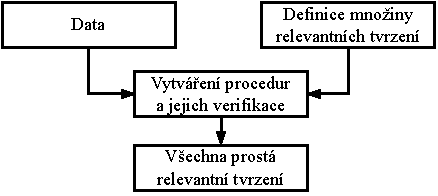
\includegraphics[width=.5\textwidth]{obrazky/GUHA/GUHA2.pdf}
    \caption{Základní postup procedury GUHA. Zdroj: vlastní.}
    \label{obr:met:GUHA2}
\end{figure}

\subsection{Důležité pojmy}


% Uvažujeme potenciálně nekonečnou množinu objektů. Metoda předpokládá výsledky existenci pozorování této množiny reprezentované v~matici dat. Cílem je získat všechny zajímavé vztahy, které jsou pravdové pro celou množinu objektů

Pro podrobnější popis procedur je nejprve třeba definovat několik pojmů, se kterými se v~procedurách pracuje. Metoda pracuje s~násdledujícími pojmy \cite{bib:GUHA}:

\begin{itemize}
    \itemsep0em
    \item \textbf{Matice dat a atributy} -- Řádky matice jsou jednotlivá pozorování. Atributem se rozumí sledovaná vlastnost, jedná se o sloupec matice.
    \item \textbf{Základní booleovský atribut} -- Jedná se o výraz $\bm{\mathrm{A(\alpha)}}$, kde $\bm{\mathrm{A}}$ je atribut a  $\bm{\alpha}$ je vlastní podmnožina $\bm{\mathrm{A}}$. $\bm{\alpha}$ může obsahovat více prvků než jeden.
    \item \textbf{Booleovský atribut} -- Každý základní boolovský atribut je booleovský atribut. Boolovské atributy jsou i negace, konjunkce a disjunkce základních boolovských atributů. 
    \item[] Pro každý řádek $i$ matice $\mathbf{M}$ nabývá boolovský atribut  $\bm{\mathrm{A}}$ hodnotu $0$, nebo $1$.
    \begin{equation*}
    \bm{\mathrm{A}}\left[i\right] = 1 \Rightarrow \mbox{boolovský atribut } \bm{\mathrm{A}} \mbox{ je pravdivý pro řádek } i.
    \end{equation*}
    \begin{equation*}
        \bm{\mathrm{A}}\left[i\right] = 0 \Rightarrow \mbox{boolovský atribut } \bm{\mathrm{A}} \mbox{ je nepravdivý pro řádek } i.
        \end{equation*}

    \item \textbf{Literál} -- Základní boolovský atribut nebo jeho negace.
    \item \textbf{Dílčí cedent} -- Konjunkce nebo disjunkce literálů.
    \item \textbf{Cedent} -- Jedná se o konjunkci dílčích cedentů. Příkladem cedentu je booleovský atribut, který vznikl konjunkcí a disjunkcí dalších atributů.

\end{itemize}


Další pojmy se týkají vztahů, se kterými procedury pracují \cite{bib:GUHA}:

\begin{itemize}
    \itemsep0em
    \item \textbf{Asociační pravidlo} -- Výraz $\mathrm{X} \rightarrow \mathrm{Y}$, kde $\mathrm{X}$ a $\mathrm{Y}$ jsou konjunkce dvojic atribut a jeho hodnota. Dále v~textu je používaná pro tento pojem zkratka AP.
    \item \textbf{Konfidence AP} -- Podíl počtu řádků, které splňují antecedent a zároveň sukcedent a počtu řádků, které splňují pouze sukcedent.
    \item \textbf{Podpora AP} -- Podíl počtu řádků, které splňují antecedent a zároveň sukcedent a počtu řádků vstupní matice dat.
\end{itemize}

Častou úlohou pro dobývání AP je nalezení všech AP, u kterých je hodnota konfidence a podpory AP větší nebo rovna danému prahu. V~rámci GUHA se AP zkoumají jako vztah dvou obecných boolovských atributů, které jsou odvozené ze sloupců vstupní matice. GUHA asociační pravidlo (GUHA AP) je 
výraz 
\begin{equation}
    \varphi \approx \psi, 
\end{equation}
kde $\varphi, \psi$ jsou boolovské atributy, které nemají obsažený žádný společný boolovský atribut. $\varphi$ se nazývá \emph{antecedent} a $\phi$ \emph{sukcedent}\footnote{Antecedent, jako cedent, který předchází a sukcedent, jako cedent, který následuje.}. Symbol $\approx$ odpovídá \emph{4ft-kvantifikátoru}, viz dále v~této sekci. Existují také podmíněná GUHA AP, která mají tvar  $\varphi \approx \psi | \chi$, kde $\chi$ je boolovský atribut.\cite{bib:GUHA}

Pravdivost GUHA AP v~matici dat $\mathbf{M}$ se určuje pomocí tzv. \emph{4ft-tabulky}. Nechť je dána matice vstupních dat $\mathbf{M}$, antecedent $\varphi$, sukcedent $\psi$. Pak \emph{4ft-tabulka} $\mathrm{4ft}(\varphi,\psi,\mathbf{M})$ je definována jako čtveřice čísel $(a,b,c,d)$, pro které platí:
\begin{itemize}
    \itemsep0em
    \item $a$ je počet řádků matice $M$, které splňují oba boolovské atributy $\varphi, \psi$.
    \item $b$ je počet řádků matice $M$, které splňují $\varphi$, ale nesplňují $\psi$.
    \item $c$ je počet řádků matice $M$, které nesplňují $\varphi$, ale splňují $\psi$.
    \item $d$ je počet řádků matice $M$, které nesplňují ani jeden atribut $\varphi, \psi$.\cite{bib:GUHA}
\end{itemize}
Reprezentace této tabulky je zobrazena v~tab. \ref*{tab:GUHA:tabulka}.

\begin{table}[hbtp!]
    \begin{center}
            \captionsetup{justification=centering}
    \caption{\emph{4ft-tabulka} matice $\mathbf{M}$ s~asociačním pravidlem $\varphi \approx \psi$.}
    \begin{tabular}{c|c|c}
        $\mathbf{M}$ & $ \;\psi \;$& $\neg\,\psi$ \\
        \hline
        $\varphi$ & $a$& $b$ \\
        \hline
        $\neg\,\varphi$ & $c$& $d$ \\
        \end{tabular}
    \label{tab:GUHA:tabulka}
\end{center}
\end{table}

\emph{4ft-kvanitifikátor}, symbol $\approx$, definuje podmínku, která se týká hodnot $(a,b,c,d)$ v~\emph{4ft-tabulce}. Kvantifikátor je formálně definovaný pomocí funkce $F_\approx$, která každé čtveřici nezáporných čísel přiřazuje hodnotu $1$, resp. $0$ pokud je, resp. není podmínka splněna. Zapisujeme $F_\approx(a,b,c,d)$ nebo zkráceně $\approx(a,b,c,d)$.\cite{bib:GUHA}
\begin{equation}
\begin{aligned}
    \mbox{GUHA AP } & \varphi \approx \psi \mbox{ je pravdivé v~matici dat }\mathbf{M} \\
    & \Leftrightarrow \approx(a,b,c,d) = 1 \mbox{, formálně zapsáno jako } \mathrm{Val}(\varphi \approx \psi) = 1.   \\
    \vspace*{.5em} \\
    \mbox{GUHA AP } & \varphi \approx \psi \mbox{ je nepravdivé v~matici dat }\mathbf{M} \\
   & \Leftrightarrow \approx(a,b,c,d) = 1 \mbox{, formálně zapsáno jako } \mathrm{Val}(\varphi \approx \psi) = 1. 
\end{aligned}
\end{equation}

Pro podmíněné AP $\varphi \approx \psi | \chi$ platí obdobné vztahy. Předpokládáme však, že boolovský atribut $\chi$ nemá ani jeden společný .atribut s~atributy $\varphi$ a $\psi$. Platí tvrzení \cite{bib:GUHA}:
\begin{equation}
    \begin{aligned}
        &\mbox{Nechť } \mathbf{M} \mbox{ je matice vstupních dat, } \varphi,\psi,\chi  \mbox{ boolovské atributy, } \approx \mbox{ kvantifikátor.} \\
        & \mbox{Podmíněné AP } \varphi \approx \psi | \chi \; \mbox{je pravdivé v~} \mathbf{M} \Leftrightarrow \varphi \approx \psi \; \mbox{ je pravdivé v~matici } \mathbf{M|}\chi.
    \end{aligned}
\end{equation}

\subsection{Procedury}
\label{sec:clever:pojmy}
V dokumentaci \cite{bib:GUHA} je popsáno sedm procedur -- \emph{4ft-Miner,  SD4ft-Miner, CF-Miner, SDCF-Miner,  KL-Miner,  SDKL-Miner,  Ac4ft-Miner} \cite{bib:GUHA}. V~knihovně v~jazyce Python jsou implementované pouze metody \emph{4ft-Miner, SD4ft-Miner, CF-Miner} \cite{bib:GUHAclever}. V~této práci jsem použila metodu pouze první metodu, proto další je další teoretický popis věnován pouze metodě \emph{4ft-Miner}.

Tato procedura pracuje s~AP $\varphi \approx \psi$, nebo s~podmíněnými AP $\varphi \approx \psi | \chi$. V~knihovně \emph{Cleverminer} lze v~hlavní funkci \texttt{cleverminer} předat vstupní DataFrame s~daty, který reprezentuje vstupní matici dat, další parametr je jedna ze tří implementovaných procedur, dále seznam podmínek pro vyhodnocení tvrzení, vypnutí optimalizace, limit pro výsledná tvrzení a seznam cedentů. Cedenty jsou rozděleny na antecedenty (parametr \texttt{ante}, tj. boolovský atribut $\varphi$), sukcedenty (parametr \texttt{succ}, tj. atribut $\psi$) a podmínky (parametr \texttt{cond}, tj. boolovský atribut $\chi$).
Každý z~boolovských atributů libovolného typu cedentu může mít tyto atributy:
\begin{itemize}
    \itemsep0em
    \item \texttt{name} -- Název příznaku matice, tj. název sloupce v~DataFramu.
    \item \texttt{type} -- Jakým pravidlem se řídí výběr více kategorií v~příznaku. Jedna z~hodnot \texttt{subset, lcut, rcut, seq, one}. 
    \item \texttt{minlen} -- Minimální počet kategorií v~daném příznaku.
    \item \texttt{maxlen} -- Maximální počet kategorií v~daném příznaku.\cite{bib:GUHAclever}
\end{itemize}

Příznaky musí být kategorické a musí být možné je seřadit. Druhá vlastnost je třeba pro vybírání více kategorií v~jednom cedentu určitými způsoby selekce. Pro textové řetězce reprezentující kategorie jsou názvy kategorií řazeny podle abecedy.\cite{bib:GUHAclever}

Pro názornost jsou dále uvedeny příklady pro jednotlivé druhy atributu \texttt{type}. Nechť je dán příznak $\mathbf{A}$ s~kategoriemi 1, 2, 3, 4, 5 a parametry jsou definovány následovně: \texttt{minlen=1}, \texttt{minlen=3}. Pokud je typ \texttt{one}, bere se jedna z~kategorií daného příznaku, tuto kategorii je třeba specifikovat. Pro typ \texttt{subset} jsou vybrány všechny následující možnosti:
\begin{itemize}
    \itemsep0em
    \item Délka je rovna 1 --  $\mathbf{A(1), A(2), A(3), A(4), A(5)}.$
    \item Délka je rovna 2 --  $\mathbf{A(1, 2), A(1, 3), A(1, 4), A(1, 5), A(2, 3), A(2, 4), A(2, 5)},$
    \item[] $\mathbf{A(3, 4), A(3, 5), A(4, 5)}.$
    \item Délka je rovna 3 --  $\mathbf{A(1, 2, 3), A(1, 2, 4), A(1, 2, 5),A(2, 3, 4), A(2, 3, 5),}$
    \item[] $\mathbf{A(3, 4, 5)}$.\cite{bib:GUHA}
\end{itemize}
Pro typ sekvence, \texttt{seq} by se pak vybraly následující možnosti:
\begin{itemize}
    \itemsep0em
    \item Délka je rovna 1 --  $\mathbf{A(1), A(2), A(3), A(4), A(5)}.$
    \item Délka je rovna 2 --  $\mathbf{A(1, 2), A(2, 3), A(3, 4), A(4, 5)}.$
    \item Délka je rovna 3 --  $\mathbf{A(1, 2, 3), A(2, 3, 4), A(3, 4, 5)}$.\cite{bib:GUHA}
\end{itemize}

Pro typ \texttt{lcut} se vybírají možnosti:
\begin{itemize}
    \itemsep0em
    \item Délka je rovna 1 --  $\mathbf{A(1)}.$
    \item Délka je rovna 2 --  $\mathbf{A(1, 2)}.$
    \item Délka je rovna 3 --  $\mathbf{A(1, 2, 3)}$.\cite{bib:GUHA}
\end{itemize}
Analogicky pro typ \texttt{rcut}.

Literály v~rámci cedentů lze také kombinovat obdobnými způsoby. Opět lze přiřa-\\dit minimální a maximální délku, typ pro kombinování literálů je výběr konjunkce, nebo disjunkce. Tyto možnosti lze specifikovat pro antecedenty, sukcedenty i pod-\\mínky. Zadání podmínek není nezbytné v~atributech funkce \texttt{cleverminer}.

Další parametry, které lze předat této funkci jsou:
\begin{itemize}
    \itemsep0em
    \item \texttt{Base} (základ) -- Minimální počet řádků, které splňují antecedenty i sukcedenty (číslo $a$ v~tabulce \ref*{tab:GUHA:tabulka}).
    \item \texttt{RelBase} (relativní základ) -- Hodnota základu vydělená celkovým počtem řádků dat (případně počtem řádků v~matici s~aplikovanou podmínkou).
    \item \texttt{conf} (Konfidence) -- Pravděpodobnost $/mathrm{P}(\psi|\varphi)$. Jinými slovy procen--\\tuální zastoupení řádků, které vyhovují $\psi$ (sukcendentům) z~těch řádků, které vyhovují i $\varphi$ (antecendtům).
    \item \texttt{AAD} (nadprůměrná závislost) -- Jak moc $\varphi$ zvyšuje  pravděpodobnost $\psi$. Kolikrát se zvýší pravděpodobnost splnění sukcedentů, když se vezmou pouze záznamy, které vyhovují antecentům, oproti všem záznamům minus 1.
    \item \texttt{BAD} (podprůměrná závislost) -- Jak moc $\varphi$ snižuje  pravděpodobnost $\psi$.
\end{itemize}

Příklad volání funkce \texttt{cleverminer} je sepsaný v~ukázce kódu č. \ref*{code:cleverminer}.
\begin{lstlisting}[language=Python, style=mystyle, label={code:cleverminer}, caption={Příklad volání funkce \texttt{cleverminer}.}]
cleverminer(df = data,
            proc = "4ftMiner", 
            quantifiers = {"conf":0.6, "Base":1000},
            ante = {
                    "attributes":
                    [
                        {
                            "name":"weekday", 
                            "type":"subset", 
                            "minlen":1, "maxlen":3
                        },
                        {
                            "name":"quarter", 
                            "type":"lcut", 
                            "minlen":1, "maxlen":4
                        }
                    ], 
                    "minlen":1, "maxlen":3, "type":"con"
                    },
            succ = {
                    "attributes":
                    [
                        {
                            "name":"L3", 
                            "type":"subset", 
                            "minlen":1, "maxlen":3
                        }
                    ], 
                    "minlen":1, "maxlen":1, "type":"con"
                    },
            cond = {
                    "attributes":
                    [
                        {
                            "name":"promo", 
                            "type":"one", 
                            "value":"promo"
                        }
                    ],
                    "minlen":1, "maxlen":1, "type":"con"
                    }
            )
\end{lstlisting}

\section{Nástroje}



\subsection{Python -- Jupyter Notebook}
Veškeré výpočty probíhaly v~jazyce Python. Metoda GUHA ve verzi Pythonu 3.10, ostatní výpočty a příprava dat ve verzi 3.9. Kód byl napsán a spouštěn v~nástroji\emph{ Jupyter Notebook}. Všechny informace o tomto nástroji jsem čerpala z~dokumentace tohoto nástroje \cite{bib:JN}. Jedná se o alternativu ke konzoli jazyka Python. Jupter Notebooky jsou interaktivní a umožňují psát a spuštět blok po \emph{buňkách}. Buňky jsou sdruženy v~souboru s~příponou \emph{ipynb}, ve skutečnosti se jedná o JSON soubor. V~souboru je uložený kód a zároveň i naposledy spuštěné výstupy jednotlivých buněk. 

Výhodou Jupyter Notebooku oproti klasické konzoli je, že podporuje odsazování, zvýrazňování syntaxe, zobrazení obrázků, HTML prvků nebo \LaTeX výrazů přímo ve výstupu pod kódem. Dále je možné soubor dobře dokumentovat pomocí jazyka Markdown. Tento značkovací jazyk není omezený jen na prostý text, jako jsou klasické komentáře v~kódu. Díky němu lze soubor strukturovat do sekcí různmách úrovní. Vytvořen je tak přehlednější kód. 

Za zmínku také stojí, že dalšími základními programovacími jazyky, které je možné spouštět v~Noteboocích jsou R a Julia. Další jazyky lze spouštět pomocí speciálního jádra pro příslušný jazyk.

S Jupyter Notebooky jsem pracovala v~editoru Visual Studio Code, který podporuje řadu programovacích jazyků. Knihovnu Cleverminer jsem spouštěla v~prostředí Google Colaboratory, které podporuje pouze Jupyter Notebooky.

\subsection*{Databáze}
Data společnosti jsou uložená v~MySQL databázi, ke které jsem přistupovala pomocí nástroje HeidiSQL, což je open-sourcový nástroj pro práci s~databázovými tabulkami. Z~tohoto programu je data možné vyexportovat do formátu CSV. S~exportovanými soubory jsem dále pracovala v~Pythonu.

\subsection{Power BI}
\label{sec:PBI}

Pro vizualizaci dat jsem použila nástroj Power BI Desktop, dále už jen Power BI. Tato aplikace umožňuje vytvořit business intelligence report pro sledovaná data. Data je možné nahrát z~různých datových zdrojů, poté z~nich vytvořit datový model. Na základě tohoto modelu pak lze vytvářet reporty s~nejrůznějšími vizuály. Aplikace má rozsáhlou online dokumentaci, a~to i v~českém jazyce. Veškeré informace o Power BI jsou čerpány z~této dokumentace \cite{bib:PBI}. 

Power BI má tři možná zobrazení -- reporty, data, model. V~reportovací části je možné vytvářet interaktivní vizualizace vstupních dat a sestavit tak i vícestránkový report. Do reportů lze přidávat vizuály pro konkrétní data a míry, upravovat vzhled a vlastnosti vizuálu. Také lze nastovat datové filtry, které se týkají buď konkrétního vizuálu, celé stránky nebo napříč celým reportem. V~sekci data jsou zobrazené všechny řádky aktuálně vybrané tabulky. Uživatel může v~tabulce vyhledávat pomocí filtrů, může přidávat nové sloupce, měnit datové typy sloupců, ale nemůže změnit hdonotu existujících dat v~tabulce. V~sekci model se nachází grafické znázornění datového modelu včetně vztahů mezi jednotlicými tabulkami a jejich sloupci. uživatel může měnit -- odebírat, přidávat, měnit kardinalitu vazeb mezi nimi.

Power BI pro práci s~daty využívá dva jazyky -- jazyk M a jazyk DAX (Data Analysis Expressions). První jmenovaný lze použít při nahrávání dat a jejich zpracování, jazyk se generuje na základě kroků v~GUI aplikace, nebo je možné psát příkazy ve vestavěném editory. Druhý jmenovaný se používá přímo ve vizualizační části pro vytváření nových sloupců a metrik, obsahuje přes 200 předdefinovaných funkcí, které jsou podobné funkcím v~aplikaci Microsoft Excel.

\subsubsection*{Nahrání dat}

Data lze do reportu nahrát tabulková data z~mnkoha typů zdrojů. Je možné se např. připojit přímo k~databázi, získat data z~webu, z~cloudového úložiště, z~textového souboru, souboru z~nástroje Microsoft Excel nebo je také možné spustit Python či R kód, který vytváří data. Nahraná data je možné předzpracovávat v~editoru Power Query, který je součástí Power BI Deskotop. Dále jsou uvedeny příklady úprav v~editoru. Je možné nastavovat záhlaví tabulky, vybírat relevantní řádky a sloupce, přidávat nové sloupce pomocí příkazu v~jazyce M. Tabulku s~daty je možné rozdělit na více tabulek, nebo naopak více tabulek sloučit do jedné, odstranit řádky s~chybějícími hodnotami nebo hodnoty nahradit. V~nástroji lze také vytvářet funkce a proměnné např. pro vygenerování tabulky kalendáře.

Editor zaznamenává provedené změny na datech. Jednotlivé kroky tak lze později případně přeskočit, upravit  nebo lze mezi úpravy vložit nový krok. Posloupnost kroků je ale důležitá, neboť kroky se provádějí postupně. Vložený krok může tedy v~některých případech způsobit chybné vykonání následujících kroků. Na obr. \ref*{obr:PBI:PQ} se nachází ukázka z~editoru Power Query.

Po uložení upravených dat v~editoru se transformovaný model zobrazí v~aplikaci Power BI, kde lze s~daty dále pracovat. Úpravu dat, který model obsahuje lze provádět pouze v~nástroji Power Query. Do editoru lze přistupovat opakovaně i během vytváření reportu, může ale nastat sitace, kdy úprava vstupních dat změní model takovým způsobem, že vizuály přestanou správně fungovat.

\begin{figure}[h!]
    \centering
    \captionsetup{justification=centering}
    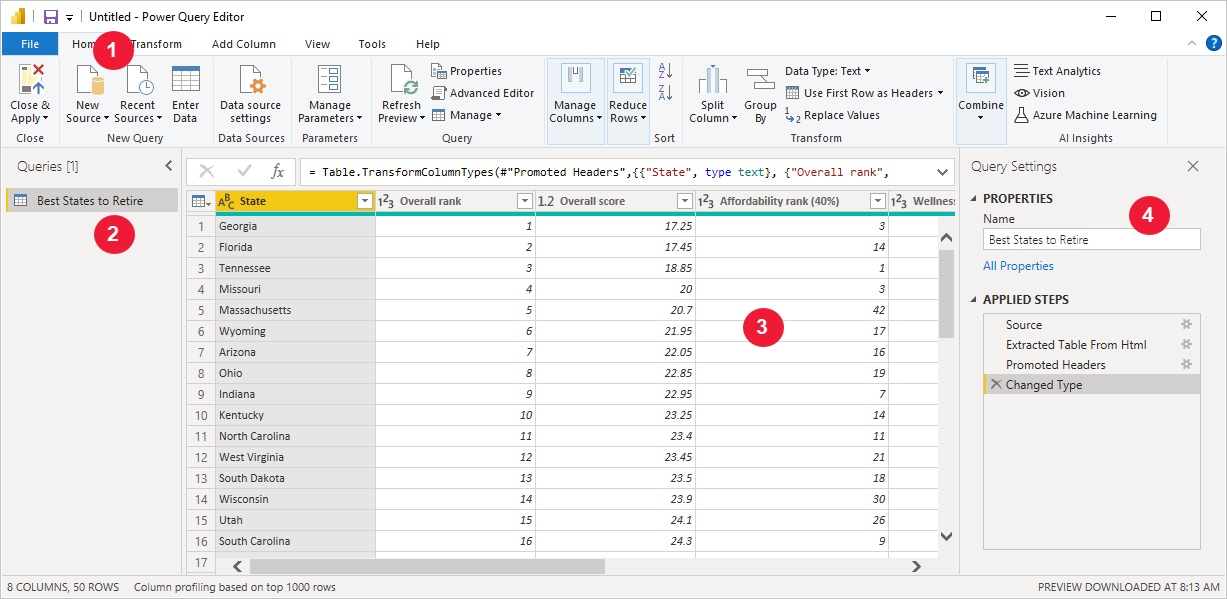
\includegraphics[width=\textwidth]{obrazky/PBIteorie/query-overview-with-data-connection.png}
    \caption{Ukázka nástroje Power Query. \\1 -- Možné interakce s~daty. 2 -- Seznam nahraných tabulek, případně proměných \\a funkcí. 3 -- Ukázka vybraných dat. 4 -- Seznam kroků a vlastností. 
    Zdroj: \cite{bib:PBI}.}
    \label{obr:PBI:PQ}
\end{figure}

\subsubsection*{Míry}

\emph{Míry}, někdy nazývané \emph{metriky} v~Power BI umožňují uživateli reportu sledovat ukazatele, které jsou relevantní pro zkoumaná data. Jedná se o výpočty na datech vytvářené pomocí jazyka DAX. Vypočítaná hodnota míry se mění podle toho, které konkrétní řádky tabulek vstupují do výpočtu, tj. jaké je vizuálu zvolená agregace a vstupní pole. K~přepočítávání dochází automaticky při interakci s~daty v~reportu. Vytvořené metriky jsou zobrazeny vedle seznamu tabulek a sloupců, které se nachází v~datovém modelu. Pro přehlednost jsou ale označeny ikonou. Z~důvodu přehlednosti je ale lepší míry přiřadit do samostatné tabulky, které neobsahuje vstupní data, ale pouze vytvořené míry.

Základní dvě možnosti jak vytvořit metriku jsou -- napsat do řádku vzorců výraz v~jazyce DAX nebo vytvořit tzv. rychlou míru pomocí dialogového okna. Rychlé míry mají ale tu nevýhodu, že nabízí pouze základní operace s~daty jako např. průměr, rozptyl, extrémy, matematické operace nebo převody datumů. 
Při vkládání dat do vizuálu jsou k~dispozici automatické míry, které se neukládají do seznamu měr v~reportu, ale vstupují pouze do vybraného vizuálu. Velmi častou používaná je míra pro počet záznamů, nebo unikátní počet záznamů.

Míru lze buď přímo vložit jako vstup do vizuálu nebo ji použít v~definici jiné míry.

\subsubsection*{Typy vizuálů}

Aplikace nabízí přes dvacet základních vizuálů a stovky vizuálů dostupných ke stažení. V~následující části jsou představeny vybrané vizuály, které jsou použité v~reportu pro data analyzovaná v~této práci. 

Základní graf je graf sloupcový, případně pruhový, které lze dále rozlišit na skládaný, skupoinový a 100\% skládaný graf. Rozdíly mezi těmito grafy jsou na obr. \ref*{obr:PBI:grafy}. Se sloupcovým grafem souvisí i graf kombinovaný, který obsahuje jak sloupce s~hodnotami, tak spojnici pro zobrazení jiných hodnot. Takový graf má tedy dvě rozdílné osy $y$, které mohou mít různá měřítka, ale pouze jednu společnou osu $x$.

\begin{figure}[h!]
    \centering
    \captionsetup{justification=centering}
    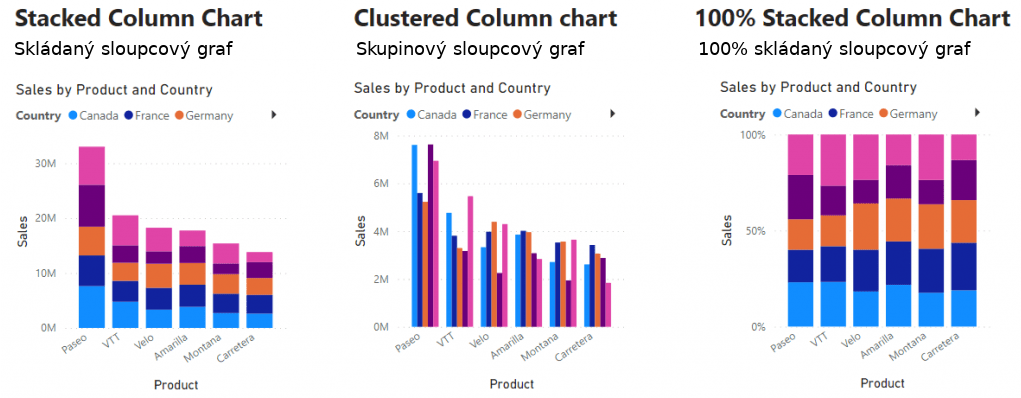
\includegraphics[width=\textwidth]{obrazky/PBIteorie/sloupcove_grafy.png}
    \caption{Základní typy sloupcových grafů. 
    Zdroj: \cite{bib:PBIgrafy}, upraveno.}
    \label{obr:PBI:grafy}
\end{figure}

Další klasický graf je graf bodový, který zobrazuje body v~průsečíku číselných hodnot $x$  a $y$. Osy mohou mít opět různá měřítka. Z bodového grafu vychází tzv. bublinový graf, který ale navíc může zobrazit ještě třetí rozměr v~datech, a to v~podobě velikosti bodů -- bublin. Tvar a poměr velikostí zobrazených bodů, resp. bublin je možné upravovat, stejně tak jejich barvu. Ukázka je na obr. \ref*{obr:PBI:grafybod}.

\begin{figure}[h!]
    \centering
    \captionsetup{justification=centering}
    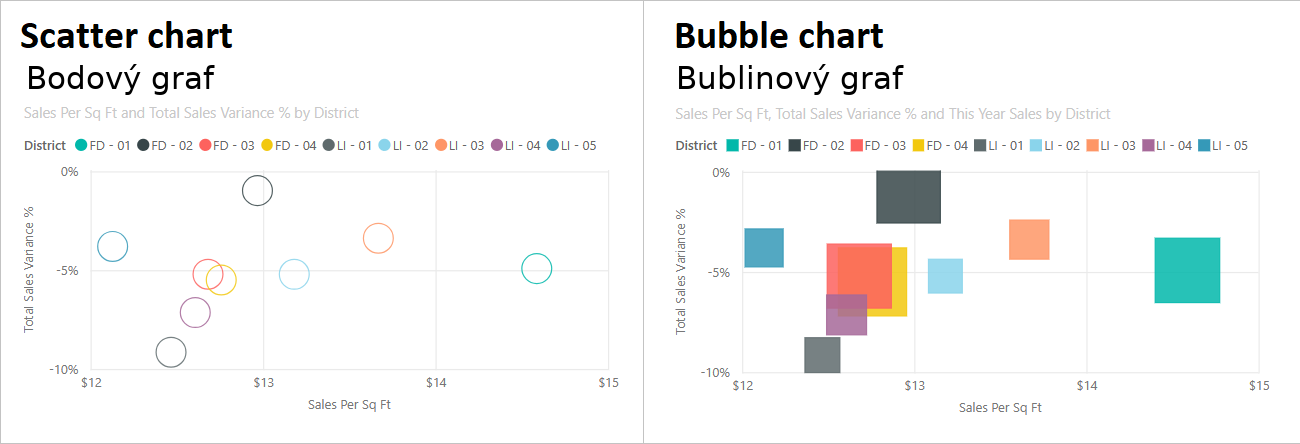
\includegraphics[width=.9\textwidth]{obrazky/PBIteorie/power-bi-compare-charts.png}
    \caption{Základní typy bodových grafů. 
    Zdroj: \cite{bib:PBI}, upraveno.}
    \label{obr:PBI:grafybod}
\end{figure}

Zajímavým vizuálem je mapa stromové struktury. Díky tomuto vizuálu je možné zachytit hierarchická data a poměrové zastoupení kategorií v~datech. Každá kategorie je reprezentována jako obdélník, označuje se pojmem větev. Každý obdélník může obsahovat své podkategorie, označené jako listy. Příklad je na obr. \ref*{obr:PBImapa}.

Formou vizuálu jsou i tabulky, matice a tzv. karty - jednočíselné nebo víceřádkové. Karty se používají pro zobrazení sledované celkové hodnoty, např. celkový počet produktů. Dále karta může obsahovat název sledované hodnoty. Příklad je uveden na obr. \ref*{obr:PBIkarty}. 
Rozdíl mezi tabulkou a maticí je ten, že tabulce lze předávat pouze sloupce a případné číselné hodnoty se spočítají podle agregace v~předchozích sloupcích. Tabulka může obsahovat záhlaví a řádek s~celkovými součty. Matice na rozdíl od obyčejné tabulky umožňuje stupňovité nahlížení na data. Pokud definujeme více vstupních sloupců z~dat jako řádky matice, lze pak záhlaví jednotlivých názvů řádků rozbalit pro větší detail. Příklad tabulky je na obr. \ref*{obr:PBItab.}. 
Příkladem vizuálu jsou i filtry, které lze zobrazit přímo vedle jiných vizuálů a které mohou ovlivnit vizuály na dané stránce. Filtr může být v~podobě dlaždic, seznamu nebo osy v~případě, že se jedná o filtrování časových údajů.

\begin{figure}[hbtp!]
    \centering
    \begin{minipage}{.4\textwidth}
        \centering
        \captionsetup{justification=centering}
        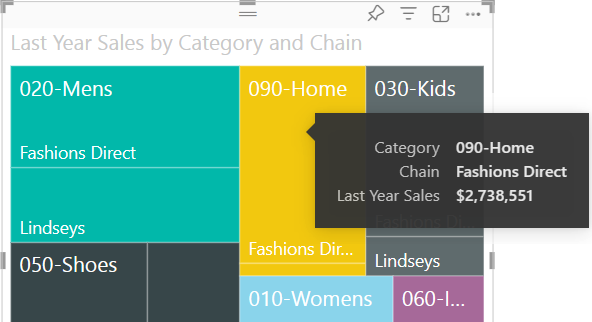
\includegraphics[width=\textwidth]{obrazky/PBIteorie/power-bi-treemap-category-tooltip.png}
        \caption{Mapa stromové struktury s~tooltipem. Zdroj: \cite{bib:PBI}.}
        \label{obr:PBImapa}
    \end{minipage}%
    \hspace*{0.4em}
    \begin{minipage}{.2\textwidth}
        \centering
        \captionsetup{justification=centering}
        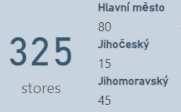
\includegraphics[width=\textwidth]{obrazky/PBIteorie/kartastoresSFF.png}
        \caption{Ukázka vizuálů jednořádková karta (vlevo) a víceřádková karta (vpravo). Zdroj: vlastní.}
        \label{obr:PBIkarty}
    \end{minipage}%
    \hspace*{0.4em}
    \begin{minipage}{.4\textwidth}
        \centering
        \captionsetup{justification=centering}
        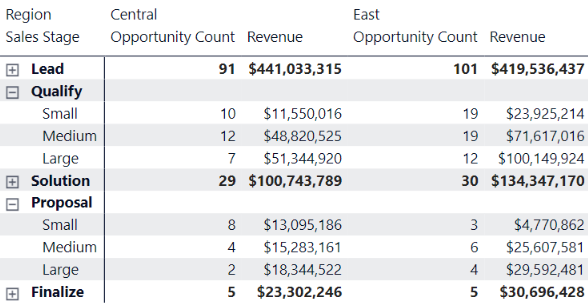
\includegraphics[width=\textwidth]{obrazky/PBIteorie/power-bi-expansion-state.png}
        \caption{Ukázka vizuálu matice. Zdroj: \cite{bib:PBI}.}
        \label{obr:PBItab.}
    \end{minipage}
\end{figure}

\subsubsection*{Vybrané funkcionality}

Ve vizuálech je možnost tooltipu, tedy zobrazení doplňující informace po najetí kurzorem myši na příslušné datové pole, viz obr. \ref*{obr:PBImapa}. Hodnoty, které se zobrazují si uživatel definuje sám. Další velmi výhodnou funkcionalitou Power BI je přechod k~podrobnostem více polí a jednoho pole. První možnost je znázorněna na obr.     \ref*{obr:PBIdrillall}. V~tomto případě se při kliknutí na ikonu $\downdownarrows$ na vizuálu zobrazí data pro další úroveň hierachie. Druhý způsob zobrazí další úroveň hierarchie, která se týká pouze jednoho vybraného pole. Pro zapnutí této volby u vizuálu je třeba zvolit volbu přechodu k~podrobnostem pro jedno pole a poté pole vybrat kurzorem myši. Stejného efektu lze docílit kliknutím pravého tlačítka myši na pole a vybrat příslušnou volbu, tím se přechod rovnou provede. Ikona $\uparrow$ v~obou případech přechází na vyšší hierarchii.

\begin{figure}[h!]
    \centering
    \captionsetup{justification=centering}
    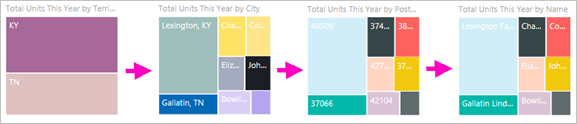
\includegraphics[width=.9\textwidth]{obrazky/PBIteorie/power-bi-drill-path.png}
    \caption{Přechod k~podrobnostem více polí. 
    Zdroj: \cite{bib:PBI}.}
    \label{obr:PBIdrillall}
\end{figure}

Křížové filtrování je další důležitá funkcionalita Power BI. Při kliknutí kurzorem myši na určité pole v~jednom vizuálu se křížově vyfiltrují pole v~ostatních vizuálech na stránce. Jinými slovy jsou odebrána všechna datová pole ve vizuálech, která se netýkají hodnoty ve vybraném poli a dojde k~přepočítání zobrazených měr a ukazatelů. Vedle křížového filtrování existuje ještě křížové zvýraznění. V~takovém případě pole ostatních, nevybraných dat z~vizuálů nezmizí, ale potlačena a vybraná data zvýrazněna. 

Nástroj Power BI disponuje mnoha dalšími funkcionalitami a vizuály, které umožňují analyzovat data a  vytvářet komplexní business intelligence reporty. Přehled všech funkcionalit této aplikace není ale předmětem této práce.

% !!!! TODO:



% \subsection{Genetický algoritmus}

% Genetický algoritmus byl inspirovaný evoluční teorií a přirozeným výběrem. Je založený na teorii, že jedinci, kteří jsou lepší než ostatní mají větší šanci na to, předat svou genetickou informaci dál. Jejich geny tk budou základem nové generace. Podobně jako ve zmíněné teorii, algoritmus používá následující informace: genetickou reprezentaci pomocí bitového  řetězce, funkci pro vyhodnocení tzv. fitness funkci, kombinování genů a mutaci. 

% Nejprve se vytvoří náhodná populace. Od této inicializační populace se postupně se iteruje dokud již další změny nevedou k~lepšímu řešení, nebo dokud neskončí počet iterací. Jedna iterace je analogií k~jedné evoluční generaci.

% Bitový řetězec populace se vyhodnotí pomocí cílové funkce (objective function). Hodnota cílové funkce pak určuje hodnotu fitness daného řešení. Fitness je možné uvažovat jako minimalizační nebo maximalizační kritérium.

% Dále se vyberou dva rodiče podle své fitness hodnoty, kteří se mezi sebou zkříží a jejich potomek vstoupí do další iterace. Jeden ze způsobů výběru je vybrat k~náhodných populací a znich vybrat populaci s~nejvyšším fitness. Křížení rodičů je pravděpodobnostní, takže v~některých případech ,ůže vzniknout potomek stejný jako jeho rodič. Obvykle se hyperparametr pro křížení se nastavuje na vyšší hodnoty např. 80 nebo 90 \%. Dalším parametrem je mutace, ta určuje zda přenesený bit zmutuje nebo ne. Jeho hodnota se nastavuje jako $1/L$, kde $L$ je délka řetězce.




\chapter{Shrink}

Cílem této práce je analyzovat shrinky produktů, které byly zaznamenány v datech dané společnosti, a zjistit příčiny jejich vzniku. V následující části je vysvětlen pojem shrink a popsány kategorie, které vybraná společnost rozeznává ve svých datech.

\section{Definice}

Slovem shrink se označuje ztráta zisku z neuskutečněného prodeje hotového produktu. Tento produkt je vyroben, či naskladněn, ale z nějakého důvodu nemohl být prodán zákazníkovi. Tímto důvodem může být například poničení produktu, jeho ztráta nebo prošlá doba spotřeby. Za shrink produktu lze označovat i stav, kdy cena produktu je neplánovaně snížena v důsledku zmíněných důvodů. Shrinkem je potom rozdíl plánované prodejní ceny a ceny, za kterou byl produkt skutečně prodán.\cite{bib:DefShrink}

% Cílem každé společnosti by mělo být tyto shrinky minimalizovat, protože kvůli shrinkům firma přichází o zisk. 


\section{Typy shrinků}
\label{sec:shrinkyTypy}

Vybraná společnost rozlišuje ve svých datech tři kategorie shrinku -- shirnky způsobené inventurou, škodami a cenové snížení. Dále se budu věnovat popisu jednotlivých typů v rámci kategorií. Každý typ má přiřazeno jednoznačné identifikační číslo, podle kterého je zaznamenáván v databázi. Z důvodů anonymizace dat v práci nejsou uvedené přesné hodnoty těchto ID, namísto toho jsou uvedeny pouze názvy, které definují shrinky.

\subsection*{Shrinky způsobené škodami}

Do kategorie shrinků způsobených škodami jsou řazeny zbylé důvody k odstranění produktu z prodeje z důvodu degradace produktu. V následující tabulce \ref{tab:sh:dam} jsou vypsané všechny typy, které moho být evidovány.

\begin{table}[hbtp!]
    \caption{Přehled jednotlivých typů shrinků z kategorie damages.}
    \label{tab:sh:dam}
    \begin{tabular}{ p{4cm} p{10.5cm}}
         Název             & Popis \\
    \hline
                Poškození               & Odpis zboží, které bylo poškozené. Např. nedopečené, spálené, špatně vyrobené nebo poškozené zaměstnancem nebo zákazníkem (kdy nelze uplatnit reklamaci na zákazníka.)       \\
                Prošlé a zkažené zboží  & Odpis zboží, kterému prošla doba spotřeby (v případě výrobků, kde je datum uvedené), zkažené či shnilé zboží (ovoce, zelenina) nebo ztvrdlé pečivo.       \\
                Zákaznické \par reklamace \strut  & Odpis zboží, které zákazník reklamoval a reklamace byla uznána, ale zároveň nelze toto zboží reklamovat u dodavatele.      \\
                Reklamace \par centrálního skladu \strut   &  Odpis zboží, které fyzicky nedorazilo z distribučního centra a nebylo možné ho reklamovat z důvodu nesplnění limitu pro vytvoření reklamace na distribučním centru. Také obsahuje odpisy neprodaných položek po ukončení výprodeje.     \\
                Kompostéry              & Odpis zboží, které je prošlé nebo poškozené a které prodejna zlikviduje v kompostéru.       \\
                Potravinová banka       & Odpis potravinářského zboží, které bylo darováno potravinovým bankám. Jedná se o produkty, které nebylo možné zařadit znovu do oběhu.    \\
                Zvířecí útulky          & Odpis potravinářského zboží, které bylo darováno do útulků zvířat. Jedná se o produkty, které nebylo možné zařadit znovu do oběhu.          \\
                Poškození vnějšími \par vlivy \strut %(internal use (err)) 
                                        & Odpis zboží, které bylo poškozeno nebo zničeno vlivem třetí strany (výbuch, vytopení, poškození majetku) nebo přírodními živly. Zboží se tedy na prodejně nenachází a nemůže proto být zlikvidováno.      \\
                Zničení & Jinak zničené zboží \\
    \end{tabular}
\end{table}

\subsection*{Shrinky způsobené inventurou}
Tato kategorie sdružuje všechny shrinky týkající se změn ve stavech zásob. Tyto změny se projeví při inventuře. V tabulce \ref*{tab:sh:inv} se nachází přehled všech evidovaných typů. Některé typy mají obdobný význam a jsou duplicitní. K tomu mohlo dajít patrnš tím, že některé subjekty používají dřívější značení pro inventuru, než jiné subjekty, které mohli přejít na nový, podorbnější způsob záznamu. 

\begin{table}[hbtp!]
    \caption{Přehled jednotlivých typů shrinků z kategorie inventory.}
    \label{tab:sh:inv}
    \begin{tabular}{ p{4cm} p{10.5cm}}
     Název             & Popis \\
    \hline
              Inventura - příjem           & Kladné připsání zboží během inventury.      \\
              Inventura - odpis           & Záporné odepsání zboží během inventury.      \\
              Inventura - velká             & Velká inventura skladu.     \\
              Inventury - oprava       & Dodatečné opravy, které bylo třeba provést po dokončení velké inventury.      \\
              Inventura - částečná    & Odpis, nebo naskladnění zboží při inventuře položek.      \\
              Neuznané reklamace \par centrálním skladem  \strut &  Odpis zboží, které bylo fyzicky dodané z centrálního skladu na prodejnu, ale prodejna jej vrátila, ale vratka nebyla uznána.     \\
              Inventura              & Starší verze ID používaného pro inventuru.\\
              Neexistující zboží     & Odpis prokazatelně ukradeného zboží nebo i ztraceného zboží.      \\
    \end{tabular}
\end{table}


\subsection*{Snížení ceny}
 
Tento typ shrinku vzniká v důsledku snížení ceny na prodejně. Tento shrink není přímo evidovaný v datech, ale lze jej vypočítat ze záznamů prodejů. Jedná se o situaci, kdy přímo na prodejně je nějaký produkt zlevněný v důsledku blížící se expirace nebo z důvodu poničení obalu. Nejedná se tak o klasickou promoakci, ale o zlevnění, které není evidováno systémem, protože se netýká všech produktů daného typu, ale pouze jednoho či několika konkrétních produktů na vybrané prodejně.

Postup pro zjištění velikosti shrinku pro jeden konkrétní produkt je následovný. Pro každou účtenku je třeba porovnat cenu každého prodaného produktu s ceníkovou cenou, případně promoční slevou. Pokud si tyto ceny nejsou rovné, pak rozdíl těchto cen je shrink daného produktu.

Vzhledem k tomu, že denně se na každé prodejně zaevidují stovky účtenek, bylo by toto postupné procházení velmi časově náročné. Zároveň tento shrink postihuje jen velmi malou část celkového prodaného objemu. Tento shrink jsem ve svých analýzách již dále nezkoumala, protože nebyl shledán prioritním. Určení příčin vzniku takového shrinku se může lišit v závislosti na konkrétních prodejnách, a to jak na zaměstnaních, které vytváří snížení cen, tak na spotřebitelích, kteří na konkrétních prodejnách nakupují.
\chapter{Zpracování dat}

Tato kapitola se zabývá popisem práce s konkrétní datovou sadou, kterou jsem obdržela. Z důvodu ochrany dat se v textu nevyskytují přesná pojmenování, ani není možné zobrazit přesnou strukturu uložení dat. 
% TODO, TBD

\section{Popis obdržených dat}

Všechna data poskytnutá společností jsou uložena v databázi, ke které byl zhotoven omezený přístup pro účely získání dat pro analýzy shrinku produktů společnosti. Zároveň s možností přístupu jsem obdržela i tabulku, která stručně komentuje všechny tabulky v databázi a sloupce v jednotlivých tabulkách. Celkem se v databázi nachází přes čtyři sta tabulek, z nichž bylo potřeba vybrat pouze ty, které obsahují relevantní data pro úlohu shrinků.

Z důvodu ochrany dat nelze uvádět přesné názvy tabulek, nicméně pro lepší orientaci v textu, každé použité tabulce přiřadím název, který odpovídá obsaženým datům v tabulce.

\subsubsection{Číselníky}

Základní číselník s údaji o produktech, se nachází v tabulce \texttt{produkt} se 27 sloupci. Pro analýzu vzniku shrinků jsem z této tabulky vybrala jako možné významné údaje následující sloupce:

\begin{itemize}
    \itemsep0em 
    \item \textbf{ID produktu}
    \item \textbf{ID prodejní varianty} -- Určuje o jaký typ balení daného produktu se jedná    
    \item \textbf{Expirace} -- Expirace produktu ve dnech (hodnoty 0, 999 a NULL označují neomezenou expiraci)
    \item \textbf{ID kategorie} -- Kategorie produktu v číselné struktuře (pro lepší interpretaci, o jakou kategorii zboží se jedná, je vhodnější použít strukturu podle úrovní, kterou lze získat napojením na tabulku \texttt{produkt\_kategorie}.)
    \item \textbf{Aktivní} --  Zda je tento produkt stále aktivní v portfoliu, nebo se jedná o produkt, který se již neprodává
\end{itemize}

Tabulka \texttt{produkt\_kategorie} obsahuje převod z číselné struktury do struktury pomocí produktové hierarchie. V obdržených datech má produktová hierarchie šest úrovní. Hierarchie produktů tvoří tedy strom se šesti úrovněmi. Nejvyšší úroveň, tj. úroveň číslo 1 má šest kategorií.

V tabulce \ref*{tab:d:4Bzast} jsou uvedeny počty podkategorií pro každou z kategorií z nejvyšší úrovně. Také je uvedeno procentuální zastoupení kategorií v nejvyšší úrovni v rámci produktového portfolia vybrané společnosti. Zastoupení je odvozeno podle počtu produktů v kategorii.

\begin{table}[hbtp!]
    \captionsetup{justification=centering}
    \begin{center}
    \caption{Počet podkategorií na jednotlivých úrovních a zastoupení \\ nejvyšší kategorie v rámci produktového portfolia.}
    \label{tab:d:4Bzast}
    \begin{tabular}{rp{4cm}  r r r r r  c}
        & Název kategorie & \multicolumn{5}{c}{Počty kategorií} &      Zastoupení kategorie      \\
        \midrule

        Úroveň: & 1       & 2    & 3   & 4   & 5    & 6    &  \\

        \midrule
        & Nepotravinářské    & 1     & 7    & 27   & 76    & 179   & 76,12\%              \\
        & Suché         & 3     & 13   & 33   & 147   & 494   & 7,28\%               \\
        & Kosmetika a drogerie        & 1     & 4    & 21   & 59    & 193   & 7,07\%               \\
        & Čerstvé       & 5     & 11   & 27   & 111   & 469   & 4,27\%               \\
        & Velmi čerstvé & 6     & 10   & 31   & 92    & 271   & 4,04\%               \\
        & Ostatní     & 4     & 4    & 4    & 5     & 5     & 1,06\%               \\
        & Tabák    & 1     & 1    & 1    & 3     & 8     & 0,17\%   \\
    \end{tabular}
    \end{center}
    \end{table}

Poslední, šestá úroveň hierarchie je přímo napojená na hodnotu číselné struktury, která je uvedena v číselníku produktů (v tabulce \texttt{produkt}). Pro získání všech úrovní kategorizace po úrovních k danému produktu je třeba vyhledat v tabulce \texttt{produkt} číselné ID kategorie daného produktu a napojit jej na poslední úroveň v tabulce produktové hierarchie (\texttt{produkt\_kategorie}). V této tabulce je pak uvedena rodičovská kategorie z úrovně 5. Poté je potřeba opět vyhledat v tabulce \texttt{produkt\_kategorie} tuto hodnotu a zjistit její nadřazenou kategorii. Takto se postupuje dokud není dosaženo nejvyšší úrovně. Tyto operace jsem provedla SQL příkazem přímo nad databází. Použila jsem vnitřní spojení na každou úroveň hierarchii na sloupce kategorie a rodičovská kategorie.

Další tabulka, se kterou jsem pracovala obsahuje informace o velikosti a hmotnosti produktů. Tato tabulka je důležitá z toho důvodu, že některé položky jsou vážené. Pokud se udává jejich množství udává se v gramech, zatímco nevážené položky jsou uvedeny v kusech. Aby bylo možné porovnávat oba číselné údaje, ke každému váženému produktu existuje přepočet na počet kusů (ozn. SKU). K tomu jsou využity údaje o počtu kusů na jednu vychystávací jednotku (dále označeno jako $SKU_{\mathrm{VJ}}$) a hmotnost jedné vychystávací jednotky daného produktu (ozn. $m_{\mathrm{VJ}}$). Vychystávací jednotka je jednotka množství používaná pro vychystávání produktů -- jeho balení a transport. Postup pro přepočet hmotnosti produktu na počet kusů ($SKU_{\mathrm{v}}$) je následovný: $$SKU = \frac{m}{m_{\mathrm{VJ}}} \cdot SKU_{\mathrm{VJ}},$$
kde $m$ je hmotnost produktu. Ze vzorce vyplývá, že může vejít neceločíselný počet kusů. Vzhledem k tomu, že tento přepočet se použije k porovnávání velikosti objemů, nikoli k objednávání zboží, tak tato skutečnost není problém.

Číselník prodejen je obsažen v tabulce \texttt{prodejny}. Vybrala jsem z tabulky následující sloupce.
\begin{itemize}
    \itemsep0em 
    \item \textbf{ID prodejny} -- Označení prodejny nebo skladu
    \item \textbf{Název} -- Název prodejny, který obsahuje název města, kde se prodejna nachází.
    \item \textbf{ID kategorie prodejny} -- Do jaké kategorie prodejna nebo sklad patří - zda se jedná o malou nebo velkou prodejnu nebo o sklad.
\end{itemize}

S číselníkem prodejen souvisí číselník pro jejich zařazení do skupin \texttt{prodejny\_skupiny}. Skupiny se mohou v čase měnit. Pro analýzu jsou relevantní tyto sloupce:
\begin{itemize}
    \itemsep0em 
    \item \textbf{ID prodejny} -- Označení prodejny nebo skladu
    \item \textbf{ID skupiny prodejen} -- Prodejny jsou sdruženy do skupin. Ty se například používají pro hromadné objednávání, nebo pro plánování promoakcí.
\end{itemize}    

Promoakce se nachází v tabulce \texttt{promoakce}. Z této tabulky jsou pro následnou analýzu potřebné údaje o ID produktu, počátečním a koncovém datu promoakce a ID skupiny prodejen, na kterých promoakce platí. Promoakce nejsou přiřazené na konkrétní prodejny, ale na skupiny prodejen. Pro další analýzy shrinků je třeba zjistit, zda byl konkrétní zaznamenaný shrink v době záznamu v promoakci, nebo ne. Z tohoto důvodu bylo potřeba tabulky spojit pomocí příkazu \texttt{JOIN} s číselníkem \texttt{prodejny\_skupiny} podle ID prodejny.

\subsubsection{Tabulky transakcí}
V tabulce \texttt{transakce} se nachází údaje o všech provedených transakcích, a to jak skladové transakce, tak prodeje a další pohyby na prodejnách. V případě prodejů prodejen jsou údaje agregované podle prodejny, konkrétního produktu a dne transakce, tzn. v této tabulce nelze rozlišit konkrétní prodeje na jednotlivých pokladnách, ale pouze souhrn za jeden den. Tabulka obsahuje údaje za posledních dvanáct měsíců.

Tabulka transakcí obsahuje 21 sloupců, jako možné podstatné sloupce pro analýzu jsem vybrala následující sloupce:

\begin{itemize}
    \itemsep0em
    \item \textbf{ID transakce} -- Jedinečné pro každou transakci.
    \item \textbf{ID produktu} -- Produkt kterého se transakce týká. Každá transakce obsahuje údaje pouze o jediném produktu. 
    \item \textbf{ID prodejny} -- Transakce je takto přiřazená prodejně, případně skladu. % Z důvodů ochrany dat jsem původní ID převedla na hodnoty od 0 do $p$, kde $p$ je počet prodejen. %TODO TBD (jo chci to tam?)
    \item \textbf{Datum transakce} -- Jedná se o obchodní datum, pokud samotná transakce proběhne až po půlnoci uvedeného dne, tak se posílá s datem z předchozího dne, neboť obchodně patří do toho dne.
    \item \textbf{ID promoce} -- Příznak zda a v jaké promoční akci se produkt nacházel v čase uvedeném v datu transakce. V rámci zpracování dat vyplynulo, že tento příznak není zcela věrohodný 
    \item \textbf{ID shrinku} -- Obsahuje označení jednotlivých typů shrinků viz sekce \ref*{sec:shrinkyTypy}. Celkem je identifikováno sedmnáct typů shrinků. V databázi tento sloupec označuje i jiná ID než ta, která se týkají shrinků, z toho plyne, že bylo třeba vyfiltrovat pouze ta data, která obsahují sedmnáct identifikačních čísel označující shrinky. % Z důvodu anonymity dat jsem původní ID přečíslovala na celočíselné hodnoty od 0 až do počtu shrinků (pro obě hlavní kategorie). %TODO TBD (jo chci to tam?)
    \item \textbf{Objem} -- Množství produktu uvedené v transakci. U kusových produktů se jedná o celočíselný údaj u vážených to je desetinné číslo.
    \item Hodnota transakce v nákladové ceně (desetinné číslo).
    \item Hodnota transakce v prodejní ceně včetně DPH -- v případě prodejů se jedná o skutečnou cenu, u zbylých transakcích je uvedena odpovídající cena podle ceníku.
\end{itemize}

Tabulku, která obsahuje údaje o jednotlivých prodejích na prodejnách společnosti, jsem pro účely této práce nazvala \texttt{transakce\_prodeje}. Celkem obsahuje třináct sloupců. Tato tabulka je vhodná pro analýzu shrinků typu snížení ceny, analýzou tohoto typu se tato práce nezabývá. Pro ostatní typy, není tato tabulka relevantní. Stejně tak není třeba zkoumat ceník jednotlivých produktů, protože v souhrnné tabulce transakcí je již uvedená hodnota transakce v prodejní ceně.

\subsubsection{Další datové zdroje}

Dále jsem pracovala s daty z databáze Českého statistického úřadu \cite{bib:czso}. Na webové stránce úřadu je dostupný odkaz ke stažení souboru ve formátu xlsx. Soubor obsahuje údaje o 237 českých městech za posledních několik desítek let. Některá města obsahují záznamy až sto let nazpět, jiné nemají tak dávno zaznamneanou historii. Dataset obsahuje údaje o lokalite, o počtu obyvatel, o sňatcích, rozvodech, stěhování obyvatel a další. V rámci přípravy dat bylo potřeba napojit prodejny k údajím o okresu, kraji a počtu obyvatel, kteří žijí v okolí prodejny. Soubor s demografickými údaji bylo třeba převést do tabulkové struktury, kde každý řádek patří jednomu městu, protože původní struktura byla nastavená, co list v souboru, to jedno město. Navíc stejné informace nejsou vždy umístěné stejně na každém listu. 


% \subsection{Období jednoho roku}

% 
Sledovala jsem tři různé veličiny, kterými lze hodnotit transakce - počet záznamů (tj. počet řádků) v tabulce \texttt{transakce}, celkové množství produktů a celková nákladová cena produktů. 

Z databáze jsem vybrala všechny transakce za rok 2022, u kterých byl evidován nějaký typ shrinku. Celkem se jednalo o %doplnit!!!
záznamů. Data jsem agregovala po jednotlivých měsících a pro každý měsíc vypočítala pomocí nástroje pivottables.


typ shrinku v závislosti na expiraci
typ shrinku v závislosti hlavní kategorii produktu
typ shrinku v závislosti na dni v měsíci
typ shrinku v závislosti na dni v týdnu

typ shrinku v závislosti na prodejně, neboli typu prodejny nebo v závislosti na centrálním skladu.
Závislost mezi prodejnami a typem produktu


\subsubsection*{Celkový přehled}

Nejprve jsem určila zastoupení jednotlivých shrinků během celého roku, a to bez uvažování závislosti na jiných faktorech. Poměr rozdělení lze vidět na obrázku \ref*{obr:rok:g:celkemD}.
Největší zastoupení, z pohledu všech tří sledovaných charakteristik, má shrink označující prošlé a zkažené zboží. Z pohledu počtu záznamů činí $70{,}24$ \% ze všech shrinků typu damage, což odpovídá 13 milionům řádkům záznamů. V případě množství neprodaných kusů produktů bylo v roce 2022 odepsáno 40 milionů kusů (tj. $65{,}67$  \%). Podle nejdůležitějšího ukazatele - nákladové ceny - tento shrink měl za následek ztrátu 635 milionů Kč (tj. $57{,}94$) \%.
Další damage shrinky, které mají zastoupení větší než 10  \% je shrink označující poškozené zboží a shrink s produkty, které byly odevzdány potravinové bance.
Zbylé shrinky mají v ročním pohledu malý počet výskytů a jejich výskyt bude analyzován v závislosti na dalších faktorech. 

\begin{figure}[hbtp!]
    \centering
    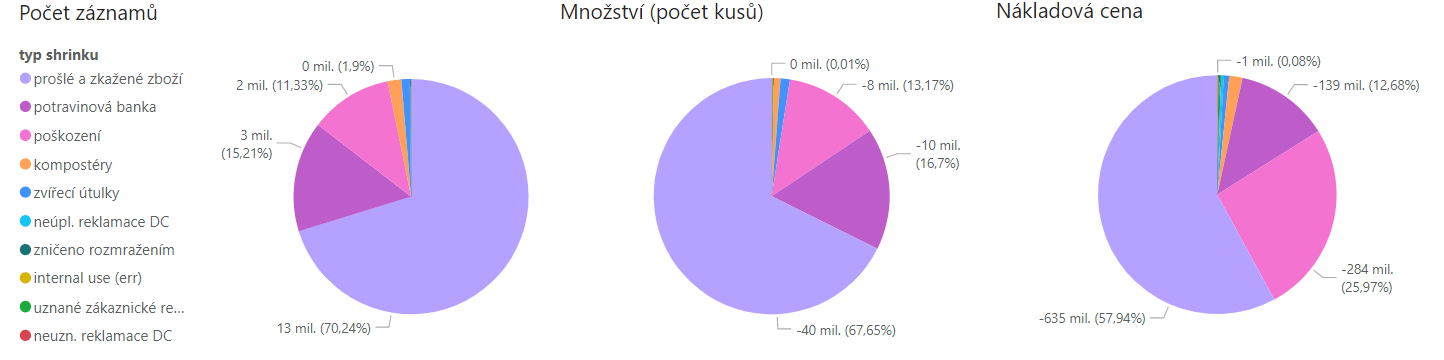
\includegraphics[width=\textwidth]{obrazky/grafy/Graf_celkem-D.png}
    \caption{Zastoupení shrinků typu damage v roce 2022.}
    \label{obr:rok:g:celkemD}
\end{figure}

\subsubsection*{Závislost typu shrinku na čase}

Porovnala jsem množství zaznamenaných shrinků v závislosti na dnech v týdnu, porovnání lze vidět na obr. \ref*{obr:rok:g:tydenD}. Jednotlivé typy jsou zastoupeny analogicky jako v souhrnném přehledu shrinků za jeden rok, tj. prošlé zboží, zboží zaslané do potravinové banky a poškozené zboží. Počty záznamů pro všechny dny jsou v rozmezí $1{,}6$ až $1{,}9$ milionů záznamů  za jeden rok. %!!! nebylo by lepsi tam dat prumer souctu za mesic za cely rok???

\begin{figure}[hbtp!]
    \centering
    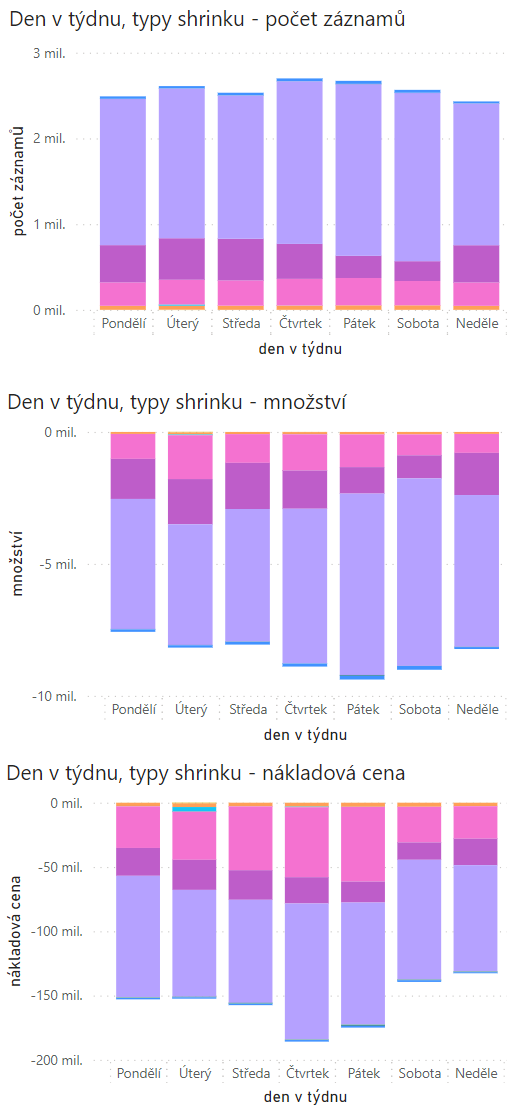
\includegraphics[width=0.5\textwidth]{obrazky/grafy/Grad_dny_tyden-D.png}
    \caption{Zastoupení shrinků typu damage v závislosti na dni v týdnu (údaje pro rok 2022).}
    \label{obr:rok:g:tydenD}
\end{figure}

\begin{figure}[hbtp!]
    \centering
    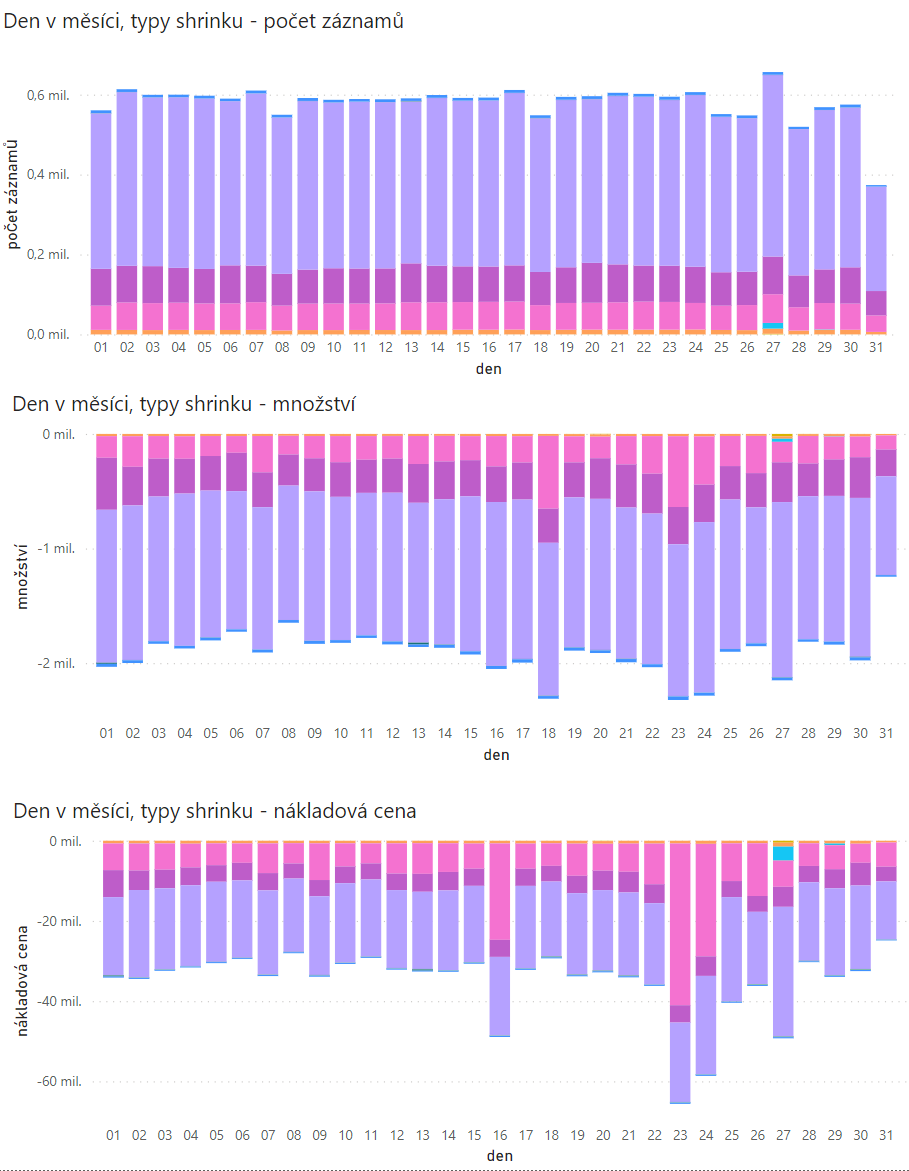
\includegraphics[width=\textwidth]{obrazky/grafy/Grad_dny_mesic-D.png}
    \caption{Zastoupení shrinků typu damage v závislosti na dni v měsíci (údaje pro rok 2022).}
    \label{obr:rok:g:mesicD}
\end{figure}

\subsubsection*{Závislost typu shrinku na hlavní kategorii zboží}

Kategorií, u které bylo evidováno nejvíce damage shrinků je kategorie produktů \emph{superfresh}. V rámci této kategorie je opět nejčastější příčinou odpisu zboží překročená doba expirace, u \emph{superfresh} produktů spíše viditelné zkažení zboží, neboť část \emph{superfresh} produktů nemá uvedenou dobu spotřeby. Druhý nejčastější shrink je shrink označující potravinovou banku. Zbylé shrinky jsou pro tuto kategorii již méně zastoupeny. Kategorie \emph{superfresh} má největší zastoupení většiny typů shrinků nad ostatními kategoriemi - přehled zastoupení jednotlivých shrinků odděleně je na obr. \ref{} %!!! udělat obrazek kde budou vedle sebe grafiký pro kazdy shrink


\subsubsection*{Závislost typu shrinku na typu prodejny}






Vzhledem k vysokému počtu dat pro jeden kalendářní rok, 
v roce 2022 bylo v databázi evidováno přes 32 milionů záznamů o týkající se shrinků
, jsem se rozhodla provést analýzu na měsíčním výběru dat z tohoto období. Jako zkoumaný měsíc jsem vybrala měsíc říjen, neboť v porovnání s letními měsíci a Vánocemi se v říjnu nevyskytují významné sezónní výkyvy.

% [2602933,
%  2439363,
%  2756406,
%  2618723,
%  2809775,
%  2624598,
%  2462898,
%  2545123,
%  2592480,
%  2712669,
%  2543758,
%  2524416]
% 31233142

Zkoumaná říjnová data obsahují $2\ 712\ 669$ řádků a patnáct sloupců. Každý řádek odpovídá jednomu záznamu v databázi shrinku daného produktu. Sledované údaje ve sloupcích jsou: 
% \subsubsection{Sledované údaje}
\begin{itemize}
    \item ID prodejny, kategorická proměnná,
    \item ID produktu, kategorická proměnná,
    \item datum transakce, kategorická proměnná,
    \item typ shrinku, kategorická proměnná,
    \item L1, kategorická proměnná,
    \item L2, kategorická proměnná,
    \item L4, kategorická proměnná,
    \item L5, kategorická proměnná,
    \item L6, kategorická proměnná,
    \item expirace, kategorická proměnná,
    \item množství, spojitá proměnná,
    \item ztracená nákladová cena, spojitá proměnná,
    \item den v týdnu, kategorická proměnná,
    \item číslo den, kategorická proměnná,
    \item období v měsíci (rozdělení měsíce na pět částí), kategorická proměnná.
\end{itemize}
Původní sloupec datum jsem rozdělila na tři jiné proměnné, a to den v týdnu, číslo dne a období v měsíci a sloupec datum jsem vynechala. Z důvodu vysokého počtu záznamů a odlišné povahy dvou typů shrinků jsem data dále rozdělila na shrinky typu damages a shrinky typu inventory. 


\subsection*{Damages shrinky}
Následující část text bude věnována rozboru dat pro shrinky typu damages.



\subsubsection{Výběr dat}
% výběr dle zastoupení shrinků a kategorií produktů a dle outlierů.

Nejprve jsem graficky analyzovala zastoupení shrinků v závislosti na vybraných proměnných pomocí nástroje Power BI, viz obr. \ref*{obr:rok:g:zastoupeni1}. V návaznosti na zjištěné zastoupení shrinků v datech jsem se rozhodla vybrat pouze ty typy shrinků, které tvoří více jak jedno procento z celkových nákladů (tj. náklady činily alespoň jeden milion korun). Vynechala jsem tedy shrinky s označením 5 až 9 a naopak shrinky 0 až 4 byly ponechány. Obdobně jsem přistupovala k záznamům i z hlediska kategorie produktu úrovně L1, jelikož z grafu je patrné, že majoritní zastoupení mají pouze dvě kategorie, a to kategorie superfresh a fresh produktů. Všechny záznamy se zbylými kategoriemi (HBC, others, nonfood, dry food a tobacco) jsem z datasetu odstranila. Těmito kroky jsem zredukovala původní počet řádků datasetu na $1\ 393\ 223$ řádků.

\begin{figure}[hbtp!]
    \centering
    \captionsetup{justification=centering}
    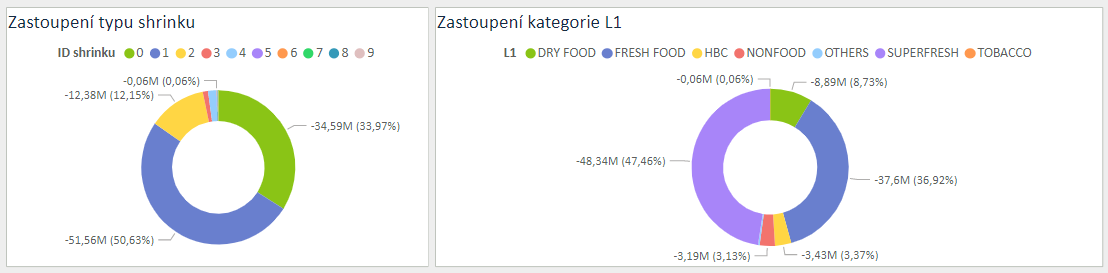
\includegraphics[width=\textwidth]{obrazky/grafy/zastoupeni1.png}
    \caption{Zastoupení shrinků typu damage a zastoupení kategorie L1 v datech \\ z října roku 2022.}
    \label{obr:rok:g:zastoupeni1}
\end{figure}

Jako cílové sloupce (\emph{target} sloupce) jsem určila sloupec s typem shrinku, množstvím produktu a nákladovou cenou. Zbylých jedenáct sloupců slouží jako vysvětlující pro-\linebreak měnné, dále budou označovány jako příznaky pro cílový sloupec. Všechny vybrané příznaky jsou kategorické proměnné, které lze dále rozdělit na nominální a ordinální. Nominální proměnné jsou ID prodejny, ID produktu, kategorie L1, L2, L4, L5 a L6. Ordinální proměnné jsou expirace, den v týdnu, číslo dne a období měsíce. Ordinální příznaky jsem přeznačila tak, aby každá obsahovala pouze hodnoty od nuly do $n_p$, kde $n_p$ je počet kategorií v $p$-tém příznaku. 

Pro další výpočty bylo vhodné přesunout se z nominálních kategorických hodnot na číselné hodnoty. Pro tyto účely jsem zvolila metodu \emph{target encoding}.  %!!! odkaz do teorie, princip meotdy je vysvětlený v kapitole...
Neboť toto kódování na numerické hodnoty zachovává velikost datového souboru, to je klíčové vzhledem k tomu, že nominální proměnné ve zkoumaných datech obsahují velký počet kategorií. Např. počet unikátních produktů v datech je $19\ 026$, což odpovídá stejnému počtu kategorií pro tuto proměnnou. Pokud bych použila one-hot kódování\footnote{One-hot kódování převádí kategorické hodnoty na numerické takovým způsobem že pro každou kategorii vytvoří samostatný sloupec s binárními hodnotami, kde 1 odpovídá dané kategorii a 0 zbylým kategoriím.}  mohlo by dojít k zásadnímu zvýšení počtu sloupců v datech, v tomto případě až o desítky tisíc. \emph{Target kódování} je podobné převodu, který jsem použila pro ordinální proměnné, ale na rozdíl od toho hodnota, která je kategorii přiřazena, souvisí se zastoupením této skupiny v cílovém sloupci a nesouvisí s uspořádáním hodnot uvnitř příznaku. Nevýhodou je, že takto upravená data mohou být náchylná na overfitting, proto je potřeba při predikování použít křížovou validaci.\cite{encoding}

% warehouse_id 339
% product_id 19026
% date_of_transaction 31
% motive_type 10
% cost_value 173409
% L1 7
% L2 20
% L4 141
% L5 450
% L6 1369
% expirace 330
% amount 48634
% weekday 7
% day 31
% quarter_of_month 5

Dále jsem se zabývala identifikací odlehlých hodnot. Nejprve jsem vizualizovala hodnoty pomocí grafu, obrázky \ref*{obr:rok:g:outlierN} a \ref*{obr:rok:g:outlierO}. Z grafu je patrné, že problémová je proměnná $warehouse\_id$, která označuje ID prodejny. Prodejny, které tvoří outliery mohou být malé prodejny, které kvůli menšímu počtu celkových produktů neevidují větší počet shrinků. % !!! jakeho grafu 

\begin{figure}[hbtp!]
    \centering
    \begin{minipage}{.5\textwidth}
        \centering
        \captionsetup{justification=centering}
        
        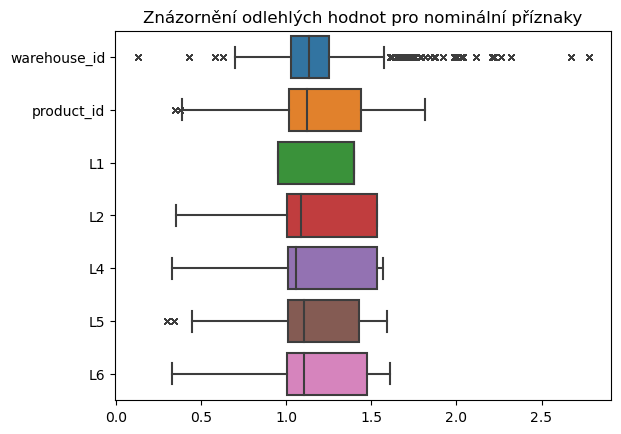
\includegraphics[width=.96\textwidth]{obrazky/zntb/box_nominal.png}
        \caption{Znázornění odlehlých hodnot pro nominální příznaky.}
        \label{obr:rok:g:outlierN}
    \end{minipage}%
    \begin{minipage}{.5\textwidth}
        \centering
        \captionsetup{justification=centering}

        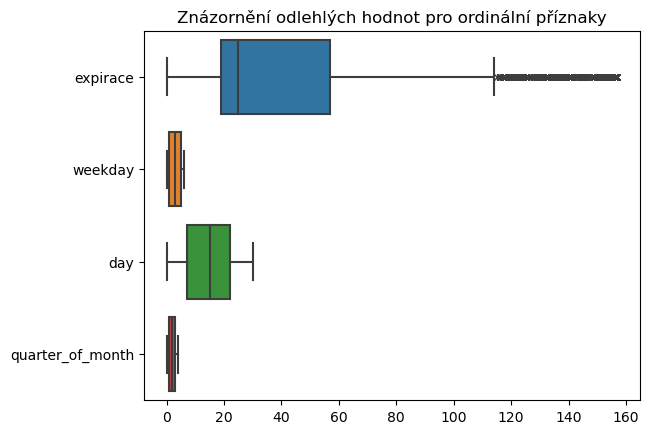
\includegraphics[width=.98\textwidth]{obrazky/zntb/box_ordinal.png}
        \caption{Znázornění odlehlých hodnot pro nominální příznaky.}
        \label{obr:rok:g:outlierO}
    \end{minipage}
\end{figure}

Pomocí Tukeyho testu jsem identifikovala přes $150\ 000$ outlierů pro příznak ID prodejny (\texttt{warehouse\_id}), čímž se dataset zredukoval na $1\ 218\ 453$ řádků. S tímto krokem klesl i počet ostatních outlierů.

V dalším kroku jsem se zaměřila na míru korelace mezi proměnnými. Vizualizovala jsem data pomocí scatter matice pro všechny proměnné, matice je možné vidět na obr. č. \ref*{obr:nb:scatter}. Z této matice můžeme na první pohled vidět, že příznaky odpovídající 4BOX kategorizaci a ID produktu vykazují závislost, což plyne z definice uspořádání této hierarchické kategorizace. V následujících krocích je cílem vybrat tu kategorii, která nejlépe popisuje data ve vztahu k shrinkům.

\begin{figure}[h!]
    \centering
    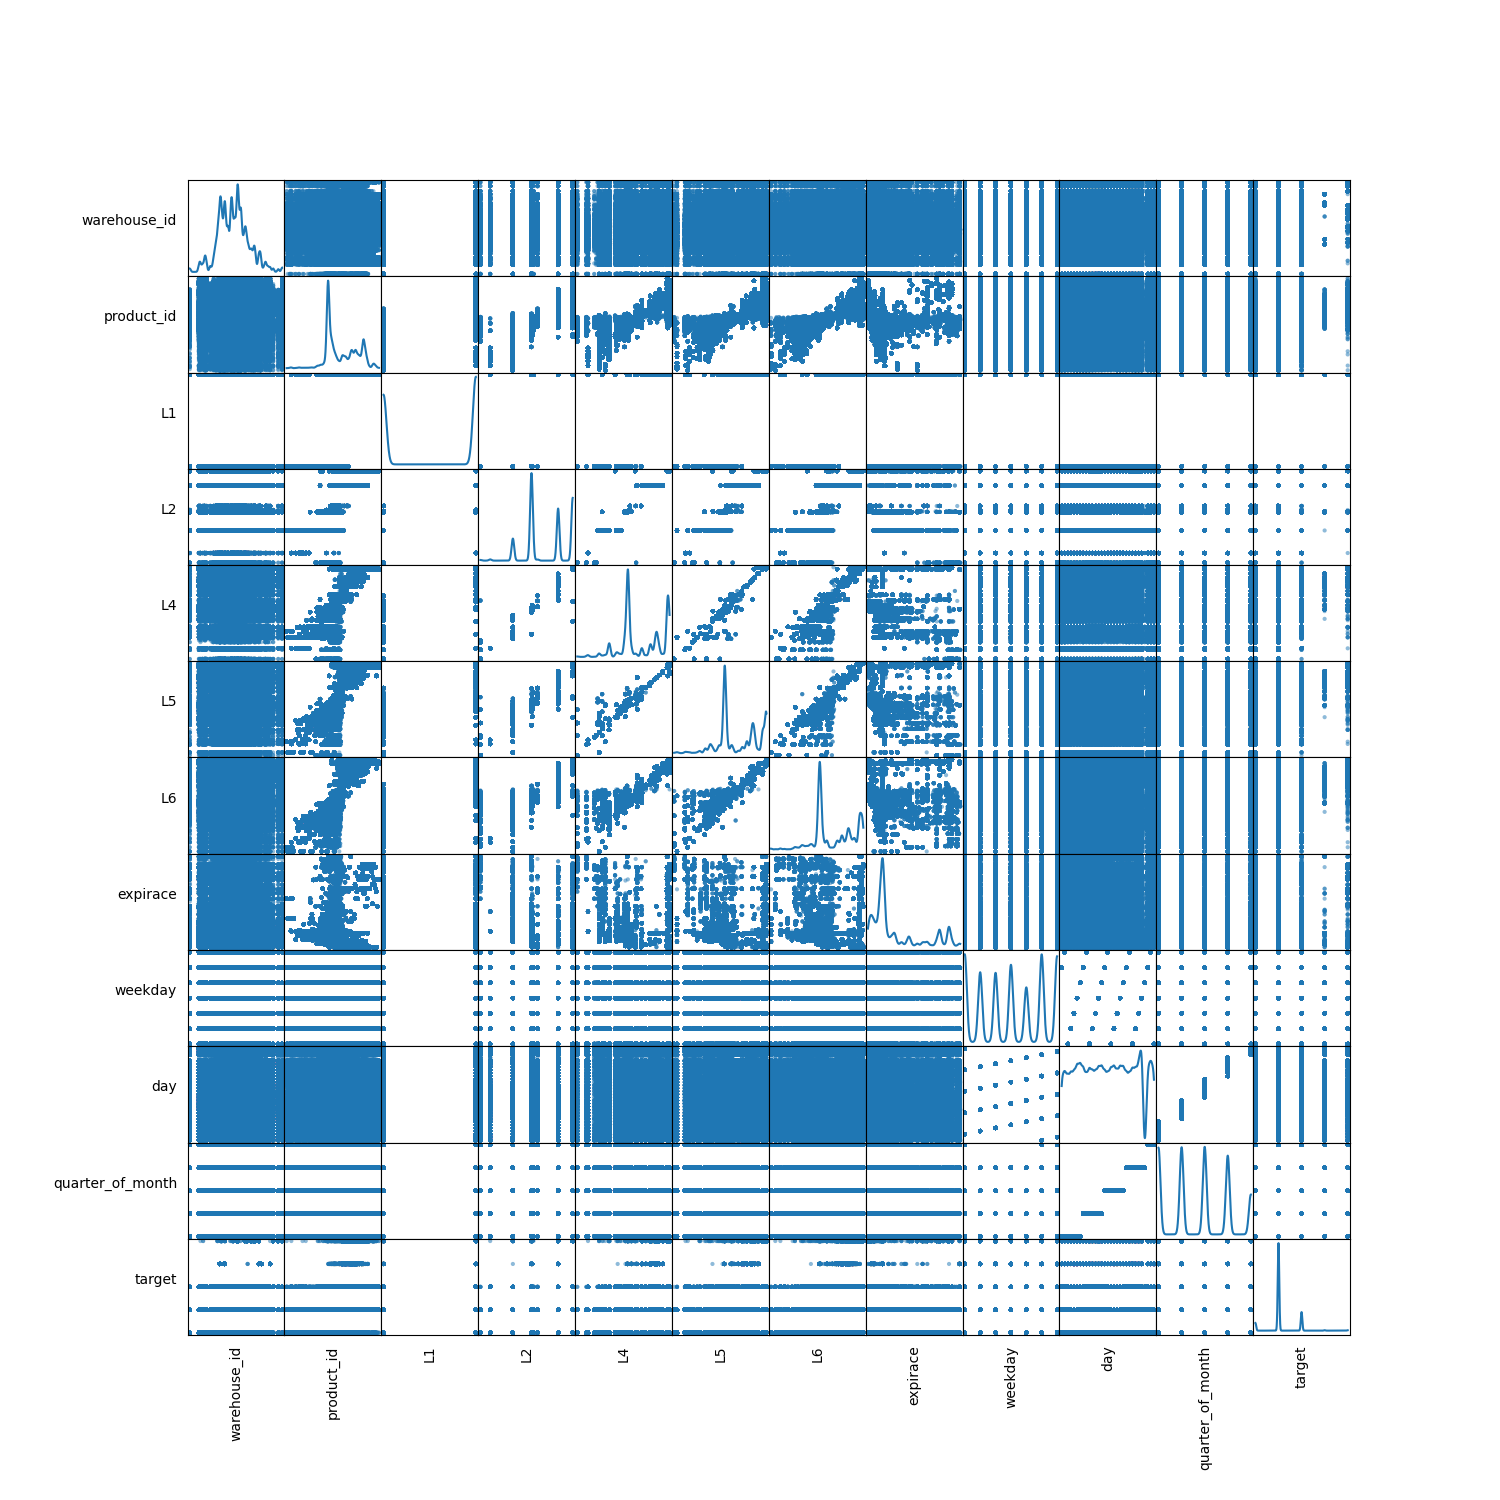
\includegraphics[width=.8\textwidth]{obrazky/zntb/MyScatter.png}
    \caption{Scatter matice příznaků.}
    \label{obr:nb:scatter}
\end{figure}
 
Jako první metodu jsem zvolila $\chi^2$ test. Vzhledem k vysokému počtu dat je matice příliš řídká, a proto nejsou výsledné hodnoty vypovídající a test je tedy pro tuto úlohu nespolehlivý.
Jiným měřítkem pro korelaci mezi proměnnými je Pearsonův korelační koeficient. %!!! odkaz na teorii
Výslednou matici popisující korelační vztahy mezi příznaky jsem vizualizovala teplotní mapou, která je zobrazena na obrázku \ref*{obr:nb:pearson}. Z výsledků je opět patrné, že mezi jednotlivými kategoriemi produktů a produkty je silná korelace. Toto zjištění je zcela logické, neboť se jedná o stromovou strukturu kategorií. Zároveň existuje korelace mezi produktovými kategoriemi a expirací produktu. p-hodnota odpovídající jednotlivým koeficientům byla vždy nulová, kromě pro koeficient týkající se dvojice proměnných expirace a ID prodejny a expirace a pořadí dne v týdnu. Je tedy možné považovat výsledky (kromě těchto dvou výjimek) za statisticky významné.

\begin{figure}[hbtp!]
    \centering
    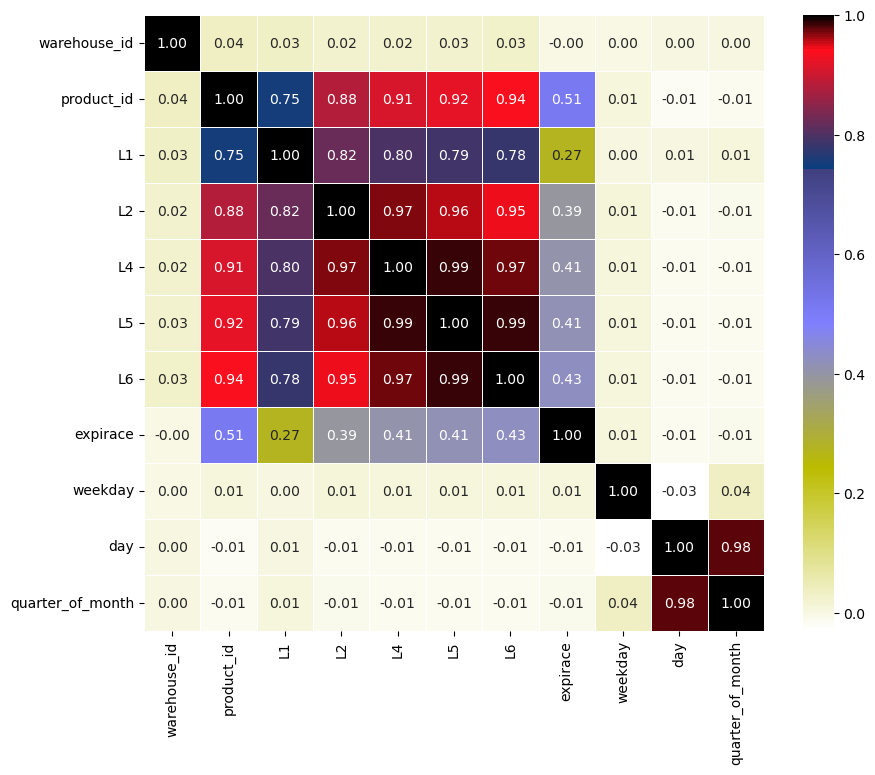
\includegraphics[width=.8\textwidth]{obrazky/zntb/pearson.png}
    \caption{Matice korelačních koeficientů mezi příznaky.}
    \label{obr:nb:pearson}
\end{figure}

Dále jsem použila výpočet koeficientů vzájemné informace \footnote{\emph{mutual information}}, který říká, jaká je podobnost mezi dvěma proměnnými \cite{bib:scikit}. % !!! odkaz na teorii
Matice vypočítaných koeficientů je na obr.\ref*{obr:nb:MI}, jelikož se jedná o symetrickou vlastnost, jsou vynechány hodnoty pod vedlejší diagonálou. Z výsledků je opět vidět zřejmé, že ID produktu sdílí úrovněmi kategorizace tím více, čím je kategorizace jemnější.

\begin{figure}[hbtp!]
    \centering
    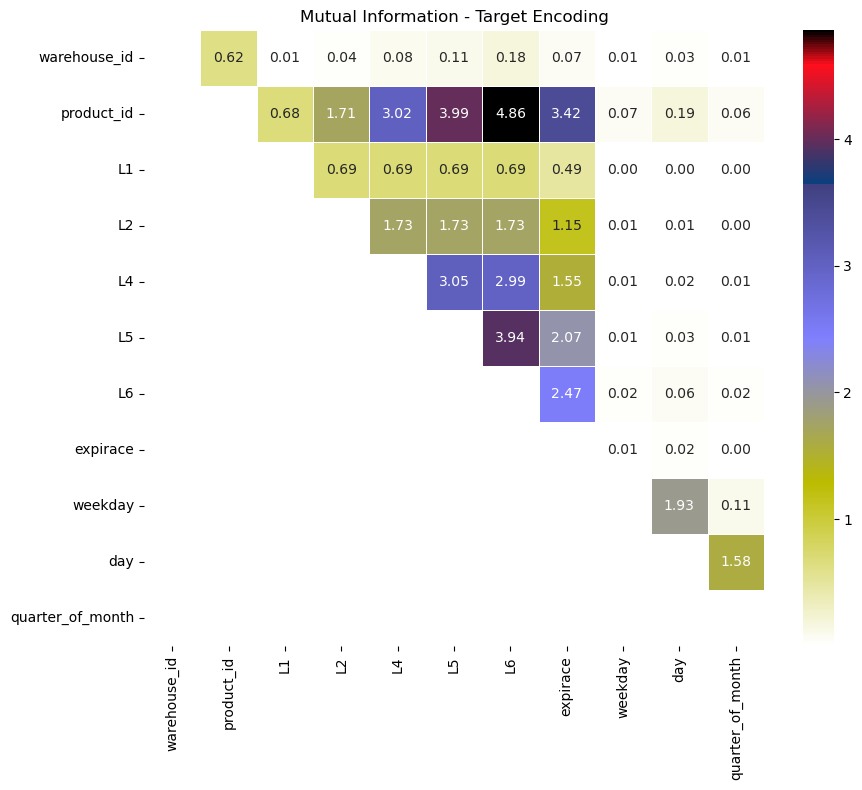
\includegraphics[width=.8\textwidth]{obrazky/zntb/MI_TE.png}
    \caption{Matice koeficientů vzájemné informace mezi příznaky.}
    \label{obr:nb:MI}
\end{figure}

%https://www.statology.org/interpret-cramers-v/
Dále jsem pro znázornění vztahu mezi proměnnými použila koeficient Cramerovo V. Koeficient jsem postupně počítala pro každou dvojici příznaků. Koeficient nabývá hodnot mezi 0 a 1. Číslo blízké nule indikuje, že mezi proměnnými není asociace, číslo blízké jedničce vysokou závislost \cite{bib:statology}. Na obr. \ref*{obr:nb:cramers} lze vidět, že pro kategorie L1 až L6 je hodnota koeficientu  po zaokrouhlení rovna jedné. Vysoká závislost je pak i mezi příznakem expirace a ID produktu a kategorií L1. Dále logicky mezi číslem dne a dnem v týdnu a obdobím v měsíci.
%!!! dopsat co to je %!!!zdroj, odkaz na teorii
\begin{figure}[hbtp!]
    \centering
    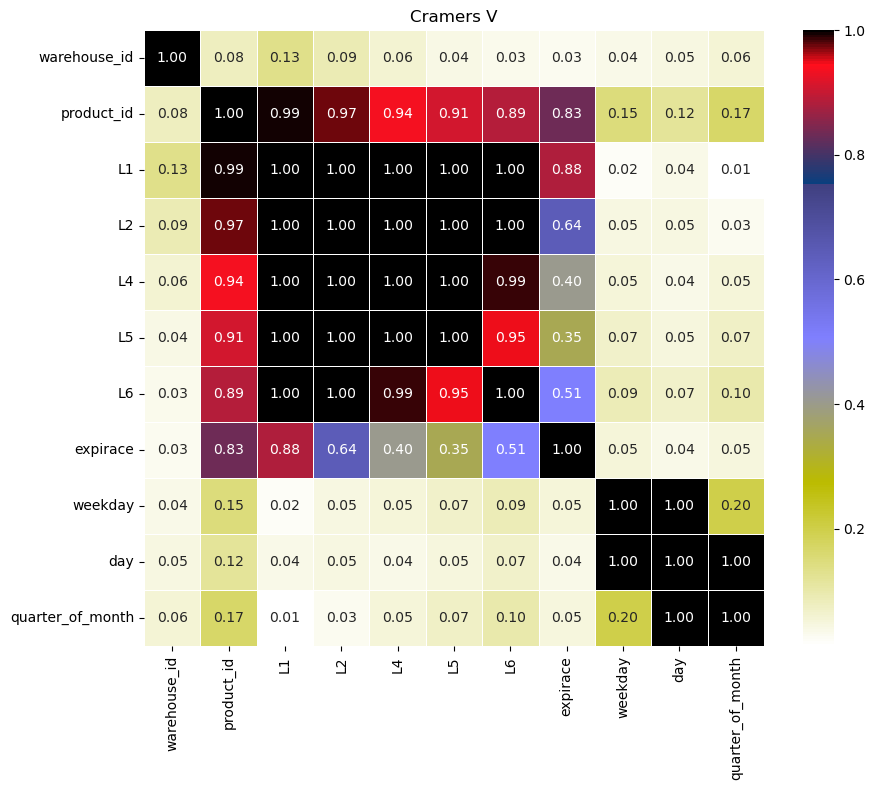
\includegraphics[width=.8\textwidth]{obrazky/zntb/cramers_u.png}
    \caption{Matice koeficientů Cramerovo V mezi příznaky.}
    \label{obr:nb:cramers}
\end{figure}

Další statistikou spočtenou na datech je Theilovo U (neboli koeficient nejistoty), který opět nabývá hodnot mezi 0 a 1 a měří vztah mezi dvěma proměnnými. Na rozdíl od předchozích statistik tento koeficient není symetrický a z výsledků lze vyvodit, ze které proměnné ze dvou zkoumaných můžeme vyvodit informaci o druhé proměnné \cite{bib:correl}. Z výsledků zobrazených v matici na obr. \ref*{obr:nb:thiels} plyne, že z ID produktu lze vyvodit část informace o kategoriích a expiraci. Zatímco úrovně L1 a L2 o ID produktu mnoho informace nenesou. Jak bylo ukázáno i v předchozích statistikách a jak vyplývá z logiky pro získání dne v týdnu a období měsíce, číslo dne nese informaci o těchto dvou příznacích.


\begin{figure}[hbtp!]
    \centering
    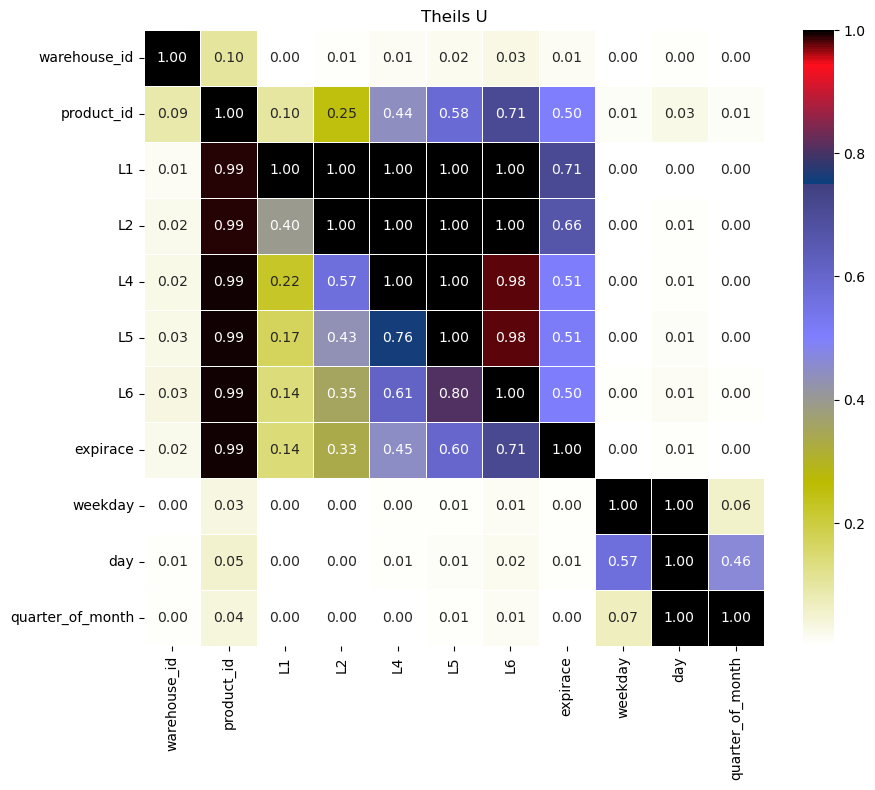
\includegraphics[width=.8\textwidth]{obrazky/zntb/theils_u.png}
    \caption{Matice koeficientů Theilovo U mezi příznaky.}
    \label{obr:nb:thiels}
\end{figure}

Z vypočítaných statistik na datasetu je patrné, že některé příznaky jsou významně závislé, a proto je třeba je z dat odstranit. Kandidáti na vynechání jsou kategorie L2, L4, L6 a číslo dne. V dalších testech budou také vybráni kandidáti a v závěru vyhodnotím, které příznaky byly podle aplikovaných metod vybrány jako vhodné k vynechání a které nikoli.

V dalším testu jsem otestovala multikolinearitu dat pomocí rozptylového inflačního faktoru (VIF). Jako hraniční faktor jsem zvolila hodnotu 40 VIF. Vysvětlující proměnné jsem odebírala z datasetu postupně a odebírání jsem ukončila až, když hodnota VIF nebyla nižší než hraniční.
Tímto došlo k redukci příznaků z jedenácti na pět, a to na kategorii L1, číslo dne, období měsíce, ID prodejny a den v týdnu. Hodnoty koeficientu VIF na datech jsou na obr. \ref*{obr:nb:vif}. 

\begin{figure}[h!]
    \centering
    \begin{minipage}{.5\textwidth}
      \centering
      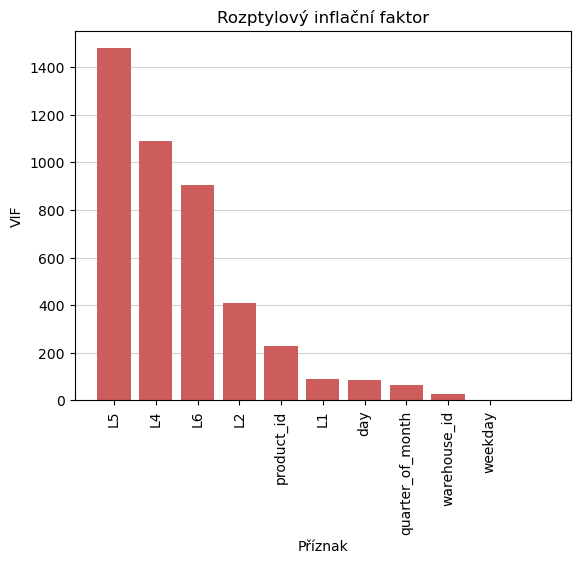
\includegraphics[width=.8\textwidth]{obrazky/zntb/VIF.png}
      \caption{Rozptylový inflační faktor.}
      \label{obr:nb:vif}
    \end{minipage}%
    \begin{minipage}{.5\textwidth}
      \centering
      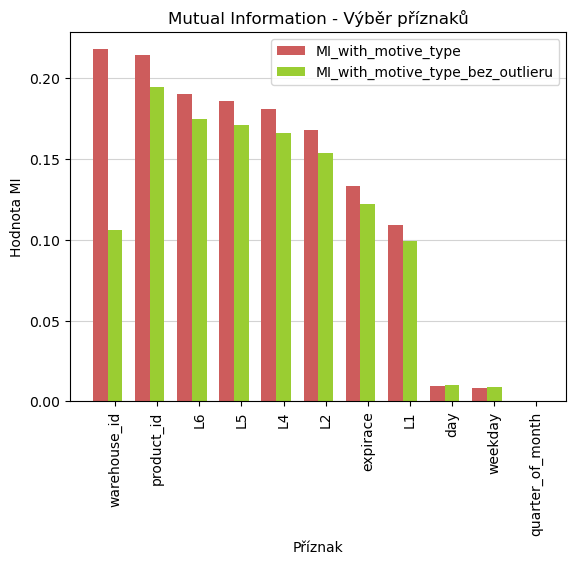
\includegraphics[width=.8\textwidth]{obrazky/zntb/MI_feature_selection.png}
      \caption{Koeficienty vzájemné informace mezi příznaky a cílovým sloupcem typ shrinku.}
      \label{obr:nb:MI_FS}
    \end{minipage}
    \end{figure}

Jako další metodu po výběr příznaků jsem vypočítala hodnotu koeficientů vzájemné informace mezi všemi příznaky s cílovým sloupcem - ID shrinku. Na obrázku \ref*{obr:nb:MI_FS} lze vidět, jak jednotlivé proměnné souvisí s cílovým sloupcem. Pro výpočet tohoto koeficientu jsem použila jak data bez outlierů, tak tenotkrát data před jejich odstraněním. Zde můžeme vidět, že významnost příznaku ID prodejny klesla o téměř polovinu. Nejvíce informace je sdíleno s ID produktu, kategorií L6, dále L5, L4, L2 a expirace. Příznaky související s časovými údaji podle tohoto kritéria nenesou mnoho společné informace.

Jako hlavní metodu pro výběr proměnných jsem se rozhodla použít metodu PCA, tuto metodu je možné použít protože kategorické proměnné jsem převedla na číselné hodnoty v předchozích krocích. Alternativou by bylo použití metody MCA, která se používá pro kategorické datasety, viz dále.
Ve své práci jsem využila implementaci PCA v knihovně \emph{Prince} v jazyce Python. 
Předtím než jsem metodu aplikovala jsem otestovala předpoklad homoskedasticity, tedy shodnost rozptylů v datech, pomocí Bartlettova testu implementovaného v knihovně \emph{factor\_analyzer}. Nulová hypotéza o shodnosti rozptylů nebyla vyvrácena (p-hodnota vyšla nulová). Metodu PCA je proto možné použít.

Na obrázcích \ref*{obr:nb:pca_roztyl_komponetn} a \ref*{obr:nb:pca_kum_roztyl_komponetn} je znázorněno prvních deset komponent a rozptyl který v datech vysvětlují. Na základě hodnot jsem vybrala prvních pět komponent. Již pátá komponenta (označená č. 4) spolu s předchozími vysvětluje více jak 95 \% variability dat. V dalším kroku jsem vypočítala příspěvky příznaků k těmto pěti komponentám a vybrala jsem ty příznaky, které přispívají nejvíce k prvním pěti komponentám. Jejich příspěvek je znázorněný na obr. \ref*{obr:nb:pca_prispevek}. Na základě výsledků analýzy hlavních komponent byly vybrány jako vhodné příznaky pro další práci s daty příznaky - příznaky ID prodejny, den v týdnu, expirace, den a období v měsíci.

\begin{figure}[h!]
    \centering
    \begin{minipage}{.5\textwidth}
      \centering
      \captionsetup{justification=centering}

      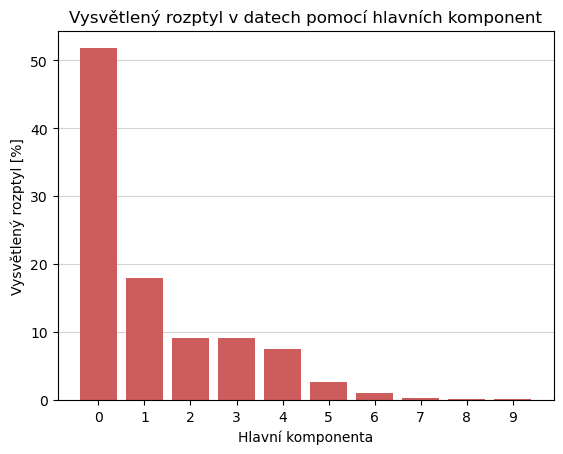
\includegraphics[width=.8\textwidth]{obrazky/zntb/pca-roztyl_komponetn.png}
      \caption{PCA - vysvětlený \\ rozptyl hlavních komponent.}
      \label{obr:nb:pca_roztyl_komponetn}
    \end{minipage}%
    \begin{minipage}{.5\textwidth}
      \centering
      \captionsetup{justification=centering}

      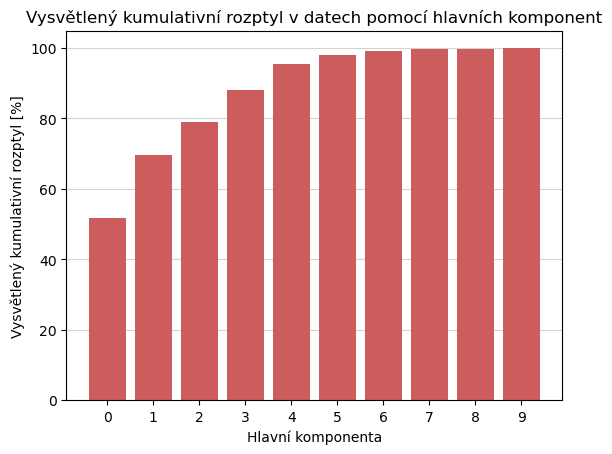
\includegraphics[width=.8\textwidth]{obrazky/zntb/pca-kum_roztyl_komponetn.png}
      \caption{PCA - kumulativní vysvětlený rozptyl hlavních komponent.}
      \label{obr:nb:pca_kum_roztyl_komponetn}
    \end{minipage}
    \end{figure}

\begin{figure}[hbtp!]
    \centering
    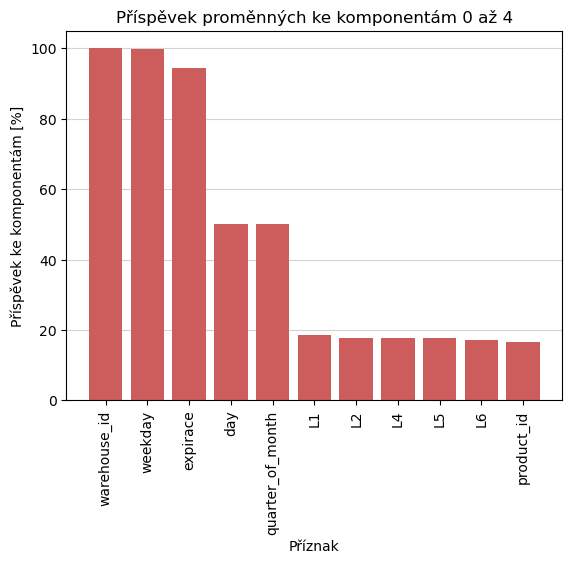
\includegraphics[width=.8\textwidth]{obrazky/zntb/pca-prispevky.png}
    \caption{Příspěvek proměnných ke komponentám 0 až 4.}
    \label{obr:nb:pca_prispevek}
\end{figure}
    
Jak již bylo zmíněno pro redukci dimenzionality u kategorických dat lze použít metodu MCA, opět jsem využila implementaci z knihovny \emph{Prince}. V této implementaci jsou nominální kategorické hodnoty kódovány tak, že narůstá počet sloupců, a proto bylo nutné, vzhledem k nárokům na paměť k uložení matice, omezit množství dat. Vybrala jsem náhodný 20\% vzorek dat, na které jsem MCA aplikovala. Vypočítala jsem prvních pět komponent, které dohromady popisují 79 \% variability dat. Jelikož byla každá kategorie chápána jako samostatná proměnná příspěvky jednotlivých příznaků ke komponentám byly rozmístěny mezi všechny kategorie, nikoli k jednotlivým příznakům. Po agregaci podle původních příznaků největší příspěvek mělo ID produktu, kategorie L6, L5, L4, zatímco nejmenší ID prodejny, L1, den v týdnu a období měsíce. Tyto výsledky je třeba brát se zvážením neboť výpočty probíhali na řádově menším vzorku než u předchozích metod.

% warehouse_id        0.024256
% product_id          1.147270
% L1                  0.035793
% L2                  0.355452
% L4                  0.841652
% L5                  0.911692
% L6                  0.930902
% expirace            0.306007
% weekday             0.035521
% day                 0.362474
% quarter_of_month    0.048981




\chapter*{Závěr} % SEM NESAHEJTE!
\addcontentsline{toc}{chapter}{Závěr} % SEM NESAHEJTE!
%
Cílem práce bylo nalézt možné příčiny vzniku shirnků produktu pro vybranou společnost a dále vytvořit prototyp řešení pro aplikování dané analýzy na data dalších společností.

V teoretické části práce jsem se seznámila s~odbornými pojmy z~odvětví logistiky a druhy plýtvání v~tomto oboru. Dále jsem sepsala princip hlavních použitých metod pro výběr proměnných a metody GUHA. Dále jsem definovala používané odborné pojmy týkající se analýzy. Teorie se také věnuje popisu nástrojů, které jsem použila při analýze. Především se jedná o popis aplikace Power BI pro vytváření interaktivních business intelligence reportů.

Samostatná kapitola se zabývá pojmem shrink. Je uvedena jeho definice a nastíněna problematika tohoto pojmu. Pak jsem popsala konkrétní typy evidovaných shrinků dané společnosti.

Nejprve jsem se seznámila s~obdrženými daty. Z rozsáhlého množství záznamů jsem vybrala vzorový měsíc s~nižším počtem záznamů, na kterém jsem prováděla všechny analýzy. Vzhledem k~velkému počtu záznamů a především vzhledem k~sezónnosti produktů a proměnlivé poptávky trhu během roku nebylo vhodné provádět analýzu na všech dostupných datech nebo na celém roku. Z databáze a externích zdrojů jsem vytipovala další data, která by pomohla vysvětlit existenci shrinků.

Stažená surová data jsem sjednotila pro další práci do samostatného datasetu. Vznikl tak dataset s~mnoha příznaky, který bylo třeba dále očistit. Odstranila jsem outliery a vybrala pouze ten typ shrinku, jehož hodnota ztracených nákladů činila nejvíce. Obdobně jsem postupovala i co se týče kategorií produktů, kterých se shrinky týkají. Z businessové stránky problému je jasné, že ke shrinku může čas od času dojít a je třeba se soustředit pouze na ty produkty, u kterých k~němu dochází opakovaně. 
Prozkoumala jsem jednotlivé příznaky datasetu a označila ty, které jsou na sobě závislé a které naopak mohou pomoci vysvětlit shrink. 

Data jsem analyzovala pomocí interaktivního reportu. Odhaleny tak byly kategorie, kterých se shrink nejvíce týká. Nejvíce postižené jsou čerstvé výrobky. Došlo také k~porovnání evidovaných shrinků mezi jednotlivými prodejnami a regiony. Ukázalo se, že umístění prodejny nemá podle dat významný vliv na vznik shrinku. 

% Na základě těchto zjištění byly stanoveny hypotézy o souvislostech vedoucích ke vzniku shrinků. Pomocí různých metod byly tyto hypotézy potvrzeny nebo vyvráceny pro konkrétní produkty.

Provedla jsem korelační analýzu, která zkoumá závislosti mezi datasetem se shrinky a tržbami. Jedná se jak o tržby shrinkovaného produktu, tak promoční tržby ostatních produktů v~kategorii definované úrovně produktové hierarchie. Korelační analýza takto dokáže rozdělit shrinkované produkty do několika kategorií v~závislosti na hodnotě korelačního koeficientu. Zde je důležité upozornit, že kauzalita vysvětlená korelací byla businessovým rozhodnutím. V~případě pochybení by následky pro společnost nebyly fatální. Naopak se jedná o postup, který společnost může snadno ovlivnit.   Společnost totiž může plánovat své promoakce s~ohledem na kategorizaci produktů. 
Korelační analýzu jsem spustila na obdržených datech a diskutovala jsem výsledky pro nejčastěji shrinkované kategorie  

V návaznosti na tuto práci by mohlo být dále otestováno celé portfolio vybrané společnosti.
Navržený způsob rozdělení produktů do kategorií podle jejich vztahu k~ostatním produktům by mohl být převeden do soběstačného nástroje, který nevyžaduje programátorský přístup a může tak být využitý například při navrhování promoakcí produktů. Tomu samozřejmě musí předcházet několikanásobné testování na datech z~více zdrojů, které ale nebyly k~dispozici pro tuto diplomovou práci.

% Bylo vyhodnoceno, kterou částí rozsáhlých dat se zabývat na základě četnosti a metod pro selekci proměnných. Prozkoumány jsou vztahy mezi jednotlivými příznaky.




%%%%%%%%%%%% SEZNAM POUŽITÝCH ZDROJŮ (LITERATURA) %%%%%%%%%%%%
\clearpage  % SEM NESAHEJTE!
\addcontentsline{toc}{chapter}{Literatura} % SEM NESAHEJTE!


	% formát: ČSN ISO 690. Můžete si to vygenerovat na http://www.citacepro.com (přihlaste se přes odkaz "ČVUT"), umí to vygenerovat TeX
	% řazení: abecedně podle autora (resp. prvního slova, není-li znám autor)

	% \bibitem{odkaz} Autor. \ti{Název knihy}. Město. Nakladatelství. Rok. 
    % \bibitem{bib:ai}


\begin{thebibliography}{1}

\bibitem{bib:Baudin}
BAUDIN, Michel. \textit{Lean Logistics: The Nuts and Bolts of Delivering Materials and Goods}. New York: Productivity Press, 2005. ISBN 978-1563272967.

\bibitem{bib:Christopher}
CHRISTOPHER, Martin. \textit{Logistics \& Supply Chain Management}. 5th ed. Harlow: Pearson Education Limited, 2016. ISBN 9781292083797.
% https://books.google.cz/books?id=NIfQCwAAQBAJ&printsec=frontcover&dq=Logistics+and+Supply+Chain+Management&hl=cs&sa=X&redir_esc=y#v=onepage&q=Logistics%20and%20Supply%20Chain%20Management&f=false

\bibitem{bib:literatura}
HASTIE, T., TIBSHIRANI R., FRIEDMAN J. H. \textit{The elements of statistical learning: data
mining, inference, and prediction.} 2nd ed. New York: Springer, 2009. Springer series in statistics. ISBN 978-0-387-84857-0.

\bibitem{bib:IIMudaipur}
What is the difference between Logistics and Supply Chain Management. In: \textit{IIM Udaipur Chronicles} [online]. 11. 10. 2019. [cit. 2022-11-07] Dostupné z: \url{https://www.iimu.ac.in/blog/what-is-the-difference-between-logistics-and-supply-chain-management/}

\bibitem{bib:Jirsak}
JIRSÁK, Petr, MERVART, Michal, VINŠ, Marek. \textit{Logistika pro ekonomy -- vstupní logistika.} 1. vydání. Praha: Wolters Kluwer ČR, 2012.

\bibitem{bib:Jones}
JONES, Daniel T., HINES Peter  a RICH Nick. Lean logistics. \textit{International Journal of Physical Distribution \& Logistics Management}. 1997, \textbf{27}(3/4), 153-173. ISSN 0960-0035. Dostupné z: doi:10.1108/09600039710170557

\bibitem{bib:PCA1}
KURITA, Takio. \textit{Principal component analysis (PCA). Computer Vision: A Reference Guide}. 2019, 1-4. [cit. 2022-11-07] Dostupné z: \url{https://link.springer.com/content/pdf/10.1007/978-3-030-03243-2\_649-1.pdf}

\bibitem{bib:PCA2}
TONHAUSEROVÁ, Zuzana. \textit{Metoda hlavních komponent a její aplikace}. Diplomová práce. Olomouc: UPOL. 2013 [cit. 2023-12-18]. Dostupné z: \url{https://theses.cz/id/iwan2b/Zuzana_Tonhauserov_-_Metoda_hlavnch_komponent.txt}

\bibitem{bib:PCA3}
JAADI, Zakaria. \textit{A Step-by-Step Explanation of Principal Component Analysis (PCA)
} [online].  [cit. 2023-03-04]. Dostupné z: \url{https://builtin.com/data-science/step-step-explanation-principal-component-analysis}


\bibitem{bib:thiel}
MILLS, Peter. \textit{Efficient statistical classification of satellite measurements}. In: \textit{International Journal of Remote Sensing.Informa UK Limited}, 2011, 32(21): 6109–6132. [cit. 2023-12-18]. Dostupné z: doi:10.1080/01431161.2010.507795

\bibitem{bib:multi}
ZAMAZAL, Petr. \textit{Statistická analýza rozsáhlých dat z průmyslu}. Diplomová práce, vedoucí Šomplák, Radovan. Vysoké účení technické v Brně, 2010.

\bibitem{bib:MCA1}
DI FRANCO, Giovanni. \textit{Multiple correspondence analysis: one only or several techniques?}. Quality \& Quantity, 2016, 50.3: 1299-1315. [cit. 2023-03-05]. Dostupné z: doi:10.1007/s11135-015-0206-0

\bibitem{bib:MCA2}
ABDI, Hervé, VALENTIN, Dominique. \textit{Multiple correspondence analysis}. In: \textit{Encyclopedia of measurement and statistics}. 2007, 2.4: 651-657. [cit. 2023-03-05]. Dostupné z: \url{https://personal.utdallas.edu/\~Herve/Abdi-MCA2007-pretty.pdf}

\bibitem{bib:MI}
NAVARA, Mirko. \textit{Teorie informace.} [online). 3. 1. 2017 [cit. 2023-12-15]. Dostupné z: \url{https://cmp.felk.cvut.cz/~navara/psi/TI_ebook.pdf}

\bibitem{bib:MI2}
PŘICHYSTAL, Jan. \textit{Úvod do teorie informace.} [online). 3. 1. 2007 [cit. 2023-12-15]. Dostupné z: \url{https://akela.mendelu.cz/~jprich/predn/teoinf.pdf}

\bibitem{bib:MI3}
KROUPA, Tomáš. \textit{Úvod do teorie informace: Matematické základy komprese a digitální komunikace.} [online). [cit. 2023-12-15]. Dostupné z: \url{https://math.fel.cvut.cz/en/people/gollova/tik/TI_prednasky.pdf}

\bibitem{bib:CA1}
GREENACRE, Michael. \textit{Correspondence analysis in practice}. chapman and hall/crc, 2017. [cit. 2023-03-05]. 

\bibitem{bib:CA2}
Correspondence analysis. In \textit{Wikiwand} [online]. [cit. 2023-03-06]. Dostupné z: \url{https://www.wikiwand.com/en/Correspondence\_analysis}

\bibitem{bib:Wronka}
WRONKA, Anna. LEAN LOGISTICS. \textit{Journal of Positive Management}. 2017, \textbf{7}(2), 55-63. ISSN 2392-1412. Dostupné z: doi:10.12775/JPM.2016.012

\bibitem{bib:seven}
SUTHERLAND Joel, BENNETT Bob. \textit{The Seven Deadly Wastes of Logistics: Applying Toyota Production System Principles to Create Logistics Value}. Bethelem, PA: Lehigh University, 2007. Dostupné z: \url{https://www.researchgate.net/publication/265356600}

\bibitem{bib:LW1}
SKHMOT, Nawras. \textit{The Lean Way Blog: The 8 Wastes of Lean. The Lean Way} [online]. 5. 8. 2017 [cit. 2022-11-17]. Dostupné z: \url{https://theleanway.net/The-8-Wastes-of-Lean}

\bibitem{bib:LW2}
SKHMOT, Nawras. \textit{The Lean Way Blog: What is Lean?. The Lean Way} [online]. 5. 8. 2017 [cit. 2022-11-17]. Dostupné z: \url{https://theleanway.net/what-is-lean}

\bibitem{bib:LW3}
SKHMOT, Nawras. \textit{The Lean Way Blog: What is Muda, Mura, and Muri?. The Lean Way} [online]. 5. 8. 2017 [cit. 2022-11-17]. Dostupné z:
 \url{https://theleanway.net/muda-mura-muri}

\bibitem{bib:DefShrink}
Learning the Lingo: 3 definitions related to unsold food inventory. In: \textit{Blog - Spoiler Alert} [online]. 17. 06. 2019. [cit. 2022-02-07] Dostupné z: \url{https://blog.spoileralert.com/3-definitions-unsold-food-inventory}

\bibitem{prince}
HALFORD, M. Prince., \textit{Prince} [online]. [cit. 2023-03-08]. Dostupné z: \url{https://github.com/MaxHalford/prince}

\bibitem{bib:encoding}
BAIJAYANTA, Roy., \textit{All about Categorical Variable Encoding } [online]. [cit. 2023-03-13]. Dostupné z: \url{https://towardsdatascience.com/all-about-categorical-variable-encoding-305f3361fd02}

\bibitem{bib:scikit}
scikit-learn Machine Learning in Python [online]. 2023 [cit. 2023-03-21]. Dostupné z: \url{https://scikit-learn.org/stable/}

\bibitem{bib:scikit-multiclass}
Multiclass and multioutput algorithms. scikit [online]. [cit. 2023-04-10]. Dostupné z: \url{https://scikit-learn.org/stable/modules/multiclass.html} 

\bibitem{bib:statology}
BOBBITT, Zach. \textit{How to Interpret Cramer's V} In \textit{Statology} [online]. 2021 [cit. 2023-03-21]. Dostupné z: \url{https://www.statology.org/interpret-cramers-v/}

\bibitem{bib:correl}
ZYCHLINSKI, Shaked. \textit{The Search for Categorical Correlation} [online]. 2018 [cit. 2023-03-14]. Dostupné z: \url{https://towardsdatascience.com/the-search-for-categorical-correlation-a1cf7f1888c9}

\bibitem{bib:MB}
HOLČÍK, Jiří, KOMENDA, Martin (eds.) a kol. \textit{Matematická biologie: e-learningová učebnice} [online]. 
1. vydání. Brno: Masarykova univerzita, 2015. [cit. 2023-03-14]. ISBN 978-80-210-8095-9.

\bibitem{bib:chooseregression}
FROST, Jim. \textit{Choosing the correct type of regression analysis.} [online]. [cit. 2023-04-10]. Dostupné z: \url{https://statisticsbyjim.com/regression/choosing-regression-analysis/}

\bibitem{bib:multiregression}
Multiclass logistic regression. In \textit{Refactored} [online]. [cit. 2023-04-10]. Dostupné z: \url{https://refactored.ai/}

\bibitem{bib:rf}
BIAU, Gérard; SCORNET, Erwan. \textit{A random forest guided tour}. In: \textit{Test} [online]. 2016, 25: 197-227. [cit. 2023-04-10].

\bibitem{bib:rfgb}
LOK, Leon. \textit{Decision trees, random forests and gradient boosting: What's the difference?} [online]. 5. 1. 2022. [cit. 2023-04-10]. Dostupné z: \url{https://leonlok.co.uk/blog/decision-trees-random-forests-gradient-boosting-whats-the-difference/}

\bibitem{bib:scipyPearson}
Scipy.stats.pearsonr. In \textit{scipy.stats.pearsonr - SciPy v1.11.4 Manual} [online]. [cit. 2023-12-10]. Dostupné z: \url{https://docs.scipy.org/doc/scipy/reference/generated/scipy.stats.pearsonr.html} 

\bibitem{bib:czso}
BILÍK, Jan. \textit{Databáze demografických údajů za vybraná města ČR} [online]. 30. 05. 2023 [cit. 2023-07-12]. Dostupné z: \url{https://www.czso.cz/csu/czso/databaze-demografickych-udaju-za-vybrana-mesta-cr}


\bibitem{bib:shrink1}
HUBER, Nicholas, MICHAEL, Katina, \textit{Minimizing Product Shrinkage across the Supply Chain using Radio Frequency Identification: a Case Study on a Major Australian Retailer,}. In: \textit{International Conference on the Management of Mobile Business (ICMB 2007)}. Toronto, ON, Canada, 2007, 45-45. [cit. 2023-12-16]. Dostupné z: doi: 10.1109/ICMB.2007.43.

\bibitem{bib:shrink2}
BECK, Adrian. \textit{Moving beyond shrinkage: developing a definition and typology of total retail loss.} 2018, 93–110. https://doi.org/10.1057/s41284-017-0090-5

\bibitem{bib:GUHA}
RAUCH, Jan, ŠIMŮNEK, Milan \textit{Metoda GUHA a Systém LISp-Miner} [online]. [cit. 2023-12-15]. Dostupné z: \url{lispminer.vse.cz}

\bibitem{bib:GUHAclever}
MASA, Petr. \textit{CleverMiner -- Beyond apriori.} [online]. [cit. 2023-12-15]. Dostupné z: \url{www.cleverminer.org}

\bibitem{bib:correlation}
de WINTER, Joost, GOSLING, Samuel, POTTER, Jeff. \textit{Comparing the Pearson and Spearman Correlation Coefficients Across Distributions and Sample Sizes: A Tutorial Using Simulations and Empirical Data. Psychological Methods.} 2016, 21: 273-290. Dostupné z: doi: 10.1037/met0000079. 

\end{thebibliography}
	
% 
	
	
% \bibliographystyle{unsrt}
% \bibliography{tex/bibliofrafie}


%%%%%%%%%%%% PŘÍLOHY PRÁCE %%%%%%%%%%%%
\newpage % SEM NESAHEJTE!
\addcontentsline{toc}{chapter}{Přílohy} % SEM NESAHEJTE!
\appendix % SEM NESAHEJTE!


%%%%%%%%%%%% Příloha A (tj. 1. kapitola v rámci příloh) %%%%%%%%%%%%

\chapter{Obsah přiloženého CD}
%
BP\_Gruberova.pdf -- soubor s elektronickou verzí této bakalářské práce.

PreprocessData -- složka se zdrojovými kódy naimplementovaného balíku \newline PreprocessData.jl.

%
% \input{priloha_A.tex} % text vkládán ze souboru, kde je i příkaz \chapter{...}


\end{document} % SEM NESAHEJTE! Konec.


